%\DeclareOption{s5paper}
%    {\setlength\paperheight {240mm}%
%     \setlength\paperwidth  {165mm}}
% S5: 165 x 242 mm (This is also called statsformat (in Swedish), it.s a special government format used in Sweden) 
% Standard format for master thesis works, according to LIU-tryck

% Packages to check out
%\usepackage{amsmath,amssymb,amsthm,amsfonts,bm}
%\usepackage{array} % for better arrays (e.g. matrices) in maths
%\usepackage{color}
%\usepackage{graphicx}
%\usepackage{float} % To get the placement H for figures
%\usepackage{tikz,pgfplots}
%\usetikzlibrary{positioning,shapes,shadows,arrows,fit, decorations}
%\usepackage[a4paper,top=1.75truecm,bottom=1.75truecm,left=1.75truecm,right=1.75truecm]{geometry}
%\usepackage[parfill]{parskip}
%\usepackage[bookmarks]{hyperref}
%\hypersetup{colorlinks=true, pagebackref=page, citecolor=blue, menucolor=red}
%\usepackage{natbib} 
%\usepackage{hypernat} 

\documentclass[]{report}
%\documentclass[a4paper]{report}
%\documentclass[s5paper]{report}

% Available sectioning commands for report: \part{}, \part{}, \chapter{}, \section{}, \subsection{}, \paragraph{}, \subparagraph{}.

% "-": Hyphen, used to join words and to separate syllables in words
% "$-$": Minus (simply use the minus sign from math mode, if not writing the entire subtraction in math mode)
% "--": En-dash, used for number ranges, to mark off nested clausees and phrases (use)
% "---": Em-dash, used to mark off nested clausees and phrases (don't use)

% Escape characters
%\& \% \$ \# \_ \{ \}
%\textasciitilde  = ~
%\textasciicircum = ^
%\textbackslash   = \

% % % % % % % % % % % % % % % % % % % % % % % % % % % % % % % % % % % % % % % % % % % % % % % %
% Warnings and their (possible) solutions
% ---------------------------------------
%
% "LaTeX Font Warning: Some font shapes were not available, defaults substituted. " -- \usepackage[T1]{fontenc} (\usepackage{t1enc} ?)
% "No file OMScmtt.fd. on input line 10." -- \usepackage[T1]{fontenc} OR \usepackage{t1enc}
% NOTE: \usepackage[T1]{fontenc} and \usepackage{t1enc} loads an ugly bitmap font by default. Install package cm-super (have not tries) using the MikTeX package manager (if you use Windows) to get around this problem, or \usepackage{lmodern} which replaces the bitmap font with teh Latin Modern font.
% % % % % % % % % % % % % % % % % % % % % % % % % % % % % % % % % % % % % % % % % % % % % % % %


% % % % % % % % % % % % % % % % % % % % % % % % % % % % % % % % % % % % % % % % % % % % % % % %
% Tips and trix
% -------------
%
% Tips for shrinking the size of the paper: http://gurmeet.net/computer-science/latex-tips-n-tricks-for-conference-papers/ (Note: I want to do the opposite)
% % % % % % % % % % % % % % % % % % % % % % % % % % % % % % % % % % % % % % % % % % % % % % % %


% % % % % % %
% PACKAGES  %
% % % % % % %

% Formatting
\usepackage[utf8]{inputenc} % Get å, ä, ö, Å, Ä, Ö
%\usepackage{t1enc} % Gets rid of the warning "No file OMScmtt.fd. on input line 10.", but loads an ugly bitmap font.
\usepackage[resetfonts]{cmap} % Help reader with interpreting ligatures (if you use cmap, you must use it before fontenc)
\usepackage[T1]{fontenc} % Gets rid of warning "No file OMScmtt.fd. on input line 10." but loads an ugly bitmap font
\usepackage{lmodern} % Replaces the default bitmap font used by t1enc and fontenc with the Latin Modern font

% Miscellaneous tools
\usepackage{etoolbox} % Includes the macro \ifstrequal
%\usepackage{xkeyval} % For enabling labeled macro arguments (see http://www.tex.ac.uk/tex-archive/macros/latex/contrib/xkeyval/doc/xkeyval.pdf)

% Abbreviations
\usepackage{abbrevs_package_with_bug_fixed} % For defining abbreviations and other stuff
\usepackage{xspace} % To prevent incorrect spacing after abbreviations

% Paper size
\iffalse
\usepackage{./Packages/s5paper/s5paper}
\fi

% Referencing
\iftrue
\usepackage[round, authoryear, comma]{natbib} % Harward style referencing
%\bibliographystyle{unsrtnat}
%\bibliographystyle{plain}
\bibliographystyle{plainnat}
\else
\usepackage[square, numbers, comma]{natbib} %
\bibliographystyle{ieeetr}
%\bibliographystyle{plain}
%\bibliographystyle{plainnat}
\fi

% Indexing
\usepackage{makeidx}
\makeindex

% Mathematics
\usepackage{mathtools}
\usepackage{amssymb} % To get \therefore (see documentation: There is no documentation :( )
\usepackage{esint} % Eddie Saudrais integrals (see documentation: http://ctan.uib.no/macros/latex/contrib/esint/esint.pdf).
% For more math symbols, see The Comprehensive LaTeX Symbol List (http://ctan.uib.no/info/symbols/comprehensive/symbols-a4.pdf)
\usepackage{cancel} % To be able to cancel out parts of an equation

% Title page
\usepackage{ifmmaketitle}

% Graphics
\usepackage{graphicx} % Necessary in order to include images
\usepackage{caption} % For captions
\usepackage{subcaption} % For subcaptions
\usepackage{tikz} % For advanced graphics functions

% Linking
\usepackage{hyperref} % Links to pages. The hyperref should generally be loaded last, with some exceptions
\usepackage{bookmark} % Ease bookmark management

% % % % % %
% MACROS  %
% % % % % %

% Naming conventions
% ------------------
%
% LaTeX does try to encourage a naming scheme:
%
% * Document level commands (\section) lowercase.
% * Package interface commands (\DeclareTextCommandDefault) CamelCase.
% * Package or kernel internal commands (\@text@composite@) lower@case@with@.
% * TeX primitives (\expandafter) lowercase.

% General macros
\newrobustcmd{\comment}[1]{}

% Flags
\newrobustcmd{\newflag}[2]{\newtoggle{#1}\settoggle{#1}{#2}}

% Document macros
\newrobustcmd{\levelname}{%
\ifnumequal{\value{subparagraph}}{0}{%
\ifnumequal{\value{paragraph}}{0}{%
\ifnumequal{\value{subsection}}{0}{%
\ifnumequal{\value{section}}{0}{%
\ifnumequal{\value{chapter}}{0}{%
\ifnumequal{\value{part}}{0}{%
}{part\xspace}%
}{chapter\xspace}%
}{section\xspace}%
}{subsection\xspace}%
}{paragraph\xspace}%
}{subparagraph\xspace}%
}

% Appearance
\newrobustcmd{\HRule}{\rule{\linewidth}{0.5mm}}
\newrobustcmd{\nspace}{\!\!}
\newrobustcmd{\blankpage}{\clearpage\thispagestyle{fancy}\renewcommand{\headrulewidth}{0pt}\chead{}\cfoot{}\IFDEBUGELSE{\begin{center}\large\textit{This page intentionally left blank}\end{center}}{\ }\clearpage}
% % % Text color
\definecolor{orange}{rgb}{1,0.5,0}
\definecolor{purple}{rgb}{0.5,0,0.5}
\definecolor{darkblue}{rgb}{0,0,0.5}
\newrobustcmd{\red}[1]{\textcolor{red}{#1}}
\newrobustcmd{\yellow}[1]{\textcolor{yellow}{#1}}
\newrobustcmd{\orange}[1]{\textcolor{orange}{#1}}
\newrobustcmd{\green}[1]{\textcolor{green}{#1}}
\newrobustcmd{\cyan}[1]{\textcolor{cyan}{#1}}
\newrobustcmd{\blue}[1]{\textcolor{blue}{#1}}
\newrobustcmd{\darkblue}[1]{\textcolor{darkblue}{#1}}
\newrobustcmd{\magenta}[1]{\textcolor{magenta}{#1}}
\newrobustcmd{\purple}[1]{\textcolor{purple}{#1}}
\newrobustcmd{\white}[1]{\textcolor{white}{#1}}
\newrobustcmd{\black}[1]{\textcolor{black}{#1}}
%\newrobustcmd{\transparent}[1]{\textcolor{transparent}{#1}}

% Table of contents
\newrobustcmd{\addtotoc}[2]{\cleardoublepage\phantomsection\addcontentsline{toc}{#1}{#2}}
% Do not add to table of contents and do not number
\newrobustcmd{\notocpart         }[3][]{\pdfbookmark[#1]{#2}{#3}\part*         {#2}}
\newrobustcmd{\notocchapter      }[3][]{\pdfbookmark[#1]{#2}{#3}\chapter*      {#2}}
\newrobustcmd{\notocsection      }[3][]{\pdfbookmark[#1]{#2}{#3}\section*      {#2}}
\newrobustcmd{\notocsubsection   }[3][]{\pdfbookmark[#1]{#2}{#3}\subsection*   {#2}}
\newrobustcmd{\notocsubsubsection}[3][]{\pdfbookmark[#1]{#2}{#3}\subsubsection*{#2}}
\newrobustcmd{\notocparagraph    }[3][]{\pdfbookmark[#1]{#2}{#3}\paragraph*    {#2}}
\newrobustcmd{\notocsubparagraph }[3][]{\pdfbookmark[#1]{#2}{#3}\subparagraph* {#2}}
% Add to table of contents but do not number
\newrobustcmd{\nonumpart         }[1]{\addtotoc{part}         {#1}\part*         {#1}}
\newrobustcmd{\nonumchapter      }[1]{\addtotoc{chapter}      {#1}\chapter*      {#1}}
\newrobustcmd{\nonumsection      }[1]{\addtotoc{section}      {#1}\section*      {#1}}
\newrobustcmd{\nonumsubsection   }[1]{\addtotoc{subsection}   {#1}\subsection*   {#1}}
\newrobustcmd{\nonumsubsubsection}[1]{\addtotoc{subsubsection}{#1}\subsubsection*{#1}}
\newrobustcmd{\nonumparagraph    }[1]{\addtotoc{paragraph}    {#1}\paragraph*    {#1}}
\newrobustcmd{\nonumsubparagraph }[1]{\addtotoc{subparagraph} {#1}\subparagraph* {#1}}

% Indexing
\newrobustcmd{\indexify}[1]{\iftoggle{ITALICIZEINDEXEDTEXT}{\textit{#1}}{#1}}
\newrobustcmd{\qindexify}[1]{#1} % For indexifying text quietly (don't do anything)

% The idx macro series
% % % Base versions
\newrobustcmd{\Bidx   }[2]{\index{#2}#1{#2}}           % The basic version of the idx macro
\newrobustcmd{\Bidxe  }[3]{\index{#2}#1{#3}}           % The extended version of the idx macro
\newrobustcmd{\Bidxp  }[3]{\index{#2}#1{#2#3}}         % The plural version of the idx macro
\newrobustcmd{\Bidxs  }[3]{\indexs{#2}{#3}#1{#2 #3}}   % The split version of the idx macro
\newrobustcmd{\Bidxse }[4]{\indexs{#2}{#3}#1{#4}}      % The split extended version of the idx macro
\newrobustcmd{\Bidxsp }[4]{\indexs{#2}{#3}#1{#2 #3#4}} % The split plural version of the idx macro
% % % Normal versions
\newrobustcmd{\idx   }[1]{\Bidx{\indexify}{#1}}           % The basic version of the idx macro
\newrobustcmd{\idxe  }[2]{\Bidxe{\indexify}{#1}{#2}}      % The extended version
\newrobustcmd{\idxp  }[2]{\Bidxp{\indexify}{#1}{#2}}      % The plural version
\newrobustcmd{\idxs  }[2]{\Bidxs{\indexify}{#1}{#2}}      % The split version
\newrobustcmd{\idxse }[3]{\Bidxse{\indexify}{#1}{#2}{#3}} % The split extended version
\newrobustcmd{\idxsp }[3]{\Bidxsp{\indexify}{#1}{#2}{#3}} % The split plural version
% % % Quite versions
\newrobustcmd{\qidx   }[1]{\Bidx{\qindexify}{#1}}           % The quite basic version of the idx macro
\newrobustcmd{\qidxe  }[2]{\Bidxe{\qindexify}{#1}{#2}}      % The quite extended version
\newrobustcmd{\qidxp  }[2]{\Bidxp{\qindexify}{#1}{#2}}      % The quite plural version
\newrobustcmd{\qidxs  }[2]{\Bidxs{\qindexify}{#1}{#2}}      % The quite split version
\newrobustcmd{\qidxse }[3]{\Bidxse{\qindexify}{#1}{#2}{#3}} % The quite split extended version
\newrobustcmd{\qidxsp }[3]{\Bidxsp{\qindexify}{#1}{#2}{#3}} % The quite split plural version macro

\newrobustcmd{\indexs}[2]{\iftoggle{REVERTINDEXORDEROFSPLITKEYS}%
{\index{#2!#1}\index{#1 #2|see{#2}}}% Index key has the reeversed order of the parts
{\index{#1 #2}\index{#2!#1|see{#1 #2}}}% Index key has the natural order of the parts
}

% Easier-to-read indexing
\newrobustcmd{\declareindexkey}     [1]{\expandafter\newabbrev\csname #1\endcsname{\idx{#1}}}
\newrobustcmd{\declareindexkeyq}    [1]{\expandafter\newabbrev\csname #1\endcsname{\qidx{#1}}}
\newrobustcmd{\declareindexkeypair} [2]{\expandafter\newabbrev\csname #2\endcsname{\idxe{#1}{#2}}}
\newrobustcmd{\declareindexkeypairq}[2]{\expandafter\newabbrev\csname #2\endcsname{\qidxe{#1}{#2}}}
%\newrobustcmd{\declareindexkeyq}[1]{\expandafter\newabbrev\csname #1\endcsname{\idxq{#1}}}
% Abbreviations
\newrobustcmd{\declareacronym} [2]{\iftoggle{INDEXACRONYMS}%
{\expandafter\newabbrev\csname #1\endcsname{\idxe{#1}{#2}\iftoggle{USEACRONYMS}{ (\qidxe{#2|see{#1}}{#1})}{}}[\iftoggle{USEACRONYMS}{\qidx{#1}}{\qidxe{#1}{#2}}]}%
{\expandafter\newabbrev\csname #1\endcsname{\idx{#2}\iftoggle{USEACRONYMS}{ (\qidxe{#1|see{#2}}{#1})}{}}     [\iftoggle{USEACRONYMS}{\qidxe{#2}{#1}}{\qidx{#2}}]}
}
\newrobustcmd{\declareacronyms}[3]{\iftoggle{INDEXACRONYMS}%
{\expandafter\newabbrev\csname #1\endcsname{\idxe{#1}{#2 #3}\index{#3!#2|see{#1}}\index{#2 #3|see{#1}}\iftoggle{USEACRONYMS}{ (#1)}{}}[\iftoggle{USEACRONYMS}{\qidx{#1}}{\qidxe{#1}{#2 #3}}]}%
{\expandafter\newabbrev\csname #1\endcsname{\idxs{#2}{#3}\iftoggle{USEACRONYMS}{ (\qidxe{#1|see{\iftoggle{REVERTINDEXORDEROFSPLITKEYS}{#3}{#2 #3}}}{#1})}{}}[\iftoggle{USEACRONYMS}{\qidxse{#2}{#3}{#1}}{\qidxs{#2}{#3}}]}
}

\newrobustcmd{\declareabbreviation} [3][]{\expandafter\newabbrev\csname #2\endcsname{#1#3}}
\newrobustcmd{\declareabbreviations}[4][]{\expandafter\newabbrev\csname #2\endcsname{#1#3 #4}}
\newrobustcmd{\declareabbreviationi} [3][]{\expandafter\newabbrev\csname #2\endcsname{#1\idx{#3}}}
\newrobustcmd{\declareabbreviationis}[4][]{\expandafter\newabbrev\csname #2\endcsname{#1\idxs{#3}{#4}}}
\newrobustcmd{\declareabbreviationqi} [3][]{\expandafter\newabbrev\csname #2\endcsname{#1\qidx{#3}}}
\newrobustcmd{\declareabbreviationqis}[4][]{\expandafter\newabbrev\csname #2\endcsname{#1\qidxs{#3}{#4}}}
\def\simpleabbrev{\declareabbreviation}
%TODO: Find some better way to denote plural form (one macro would be better since acronyms are indexed verbosely only ocne)
% Allow pluralform of abbreviations
%\newrobustcmd{\s}  {\nspace s\xspace} % For abbreviations that are not indexed
%\newrobustcmd{\qsi}{\nspace\qindexify{s}\xspace} % For abbreviations that are indexed quietly
%\newrobustcmd{\si} {\nspace\indexify{s}\xspace} % For abbreviations that are indexed verbosely

% Mathematics
\newrobustcmd{\opd}[0]{\operatorname{d}} % Used e.g. in integrals and derivatives
\newrobustcmd{\normal}[0]{\normvec{n}} % Used e.g. in integrals and derivatives
\newrobustcmd{\range}[2]{#1{--}#2}

% DEBUG is defined in options.tex
\newrobustcmd{\IFDEBUG        }[1]{\iftoggle {DEBUG}{#1}{  }}
\newrobustcmd{\IFDEBUGELSE    }[2]{\iftoggle {DEBUG}{#1}{#2}}
\newrobustcmd{\IFNOTDEBUG     }[1]{\nottoggle{DEBUG}{#1}{  }}
\newrobustcmd{\IFNOTDEBUGHELSE}[2]{\nottoggle{DEBUG}{#1}{#2}}

% PAPERPRINT is defined in options.tex
\newrobustcmd{\IFPAPERPRINT        }[1]{\iftoggle {PAPERPRINT}{#1}{  }}
\newrobustcmd{\IFPAPERPRINTELSE    }[2]{\iftoggle {PAPERPRINT}{#1}{#2}}
\newrobustcmd{\IFNOTPAPERPRINT     }[1]{\nottoggle{PAPERPRINT}{#1}{  }}
\newrobustcmd{\IFNOTPAPERPRINTHELSE}[2]{\nottoggle{PAPERPRINT}{#1}{#2}}

% % % % % % % % % % % % % % % % % % % %
% OPTIONS FOR COMPILING THE DOCUMENT  %
% % % % % % % % % % % % % % % % % % % %
% % % % % % % % % % % % % % % % % % % % % % % % % % % % % % % % % % % % % % % % % % % % % % % %
% Options.tex
% -----------
%
% This file contains all options that can be tuned throughout the document. This is the only file that should contain any parameters that can be changed or adjusted in order to tune the document.
% % % % % % % % % % % % % % % % % % % % % % % % % % % % % % % % % % % % % % % % % % % % % % % %


% % % % % % % % % % % % % % % % % % % % % % % % % % % % % % % % % % % % % % % % % % % % % % % %
% Dimensions
% ----------
%
% (see http://nwalsh.com/tex/texhelp/Plain.html#dimensions, http://en.wikipedia.org/wiki/Point_%28typography%29)
%
% pt: Point
% pc: pica (12 pt)
% in: inch (72.27 pt)
% bp: Big point (72 bp = 1 in)
% cm: Centimeter
% mm: Millimeter
% dd: Didot point
% cc: cicero (12 dd)
% sp: Scaled point (65,536 sp = 1 pt), the smallest TeX unit
% ex: Nomimal x-height
% em: Nominal m-width (M-width?)
%
%   Available in math mode:
%
% mu: math unit, 1 em = 18 mu, where em is taken from the math symbols family, various lengths are derived from it (thinspace, thickspace, etc.)
%
%   Additionally available in pdfTeX and LuaTeX:
%
% px: "pixel", the dimension given to the \pdfpxdimen primitive; default value is 1 bp, corresponding to a pixel density of 72 dpi
% % % % % % % % % % % % % % % % % % % % % % % % % % % % % % % % % % % % % % % % % % % % % % % %


% % % % % % % % % % % % % % % % % % % % % % % % % % % % % % % % % % % % % % % % % % % % % % % %
% Spacings in math mode
% ---------------------
%
% \,       thin space (normally 1/6 of a quad)
% \> or \: medium space (normally 2/9 of a quad)
% \;       thick space (normally 5/18 of a quad)
% \!       negative thin space (normally 1/6 of a quad)
%
% TexXBook definition: \def\,{\mskip\thinmuskip} \def\!{\mskip-\thinmuskip}
%
% \thinmuskip would normally be .16667em (= 3 mu), though it might be redefined.
%
% \quad    usually 1em (derived from identities above)
% % % % % % % % % % % % % % % % % % % % % % % % % % % % % % % % % % % % % % % % % % % % % % % %



% % % % % %
% FLAGS   %
% % % % % %

% DEBUG (should be false when publishing or simulating publishing, true otherwise)
% Affects: Extra information written into the document
\newflag{DEBUG}{true} % For debugging the document
%\newflag{DEBUG}{false} % For publishing the document

% PAPERPRINT (should be true if the compiled document is intended to be printed to paper, false otherwise)
% Affects: Link colors
%\newflag{PAPERPRINT}{true} % For debugging the document
\newflag{PAPERPRINT}{false} % For publishing the document

% Miscellaneous flags
\newflag{SKPIPLINEBETWEENPARAGRAPHS} {true}  % Controls whether a line is skipped between paragraphs
\newflag{ITALICIZEINDEXEDTEXT}       {false}  % Controls whether indexed text becomes italicized in the body text
\newflag{USEACRONYMS}                {true}  % Controls whether acronyms should be used or not
\newflag{INDEXACRONYMS}              {true}  % Controls whether the acronyms or the full forms get indexed
\newflag{REVERTINDEXORDEROFSPLITKEYS}{false}  % Controls which is the main index key for split keys
\newflag{SCRIPTSIZEINDEX}            {false}  % Controls the size of the index
\newflag{SCRIPTSIZEBIBLIOGRAPHY}     {false}  % Controls the size of the bibliography

% Debug options
\newflag{INDEXEDTEXTPURPLE}          {\iftoggle{DEBUG}{true}{false}}  % Controls whether indexed text becomes purple in the body text
%\newflag{INDEXEDTEXTPURPLE}          {false}  % Controls whether indexed text becomes purple in the body text
%\newflag{PRINTLABLES}                {\iftoggle{DEBUG}{true}{false}}  % Controls whether indexed text becomes purple in the body text
\newflag{PRINTLABLES}                {false}  % Controls whether indexed text becomes purple in the body text

% % % % % % % %
% APPEARANCE  %
% % % % % % % %

% Names
\renewcommand{\contentsname}{Table of Contents} % Rename Contents to Table of contents

% Names possible to change
%
% \abstractname   Abstract
% \alsoname       see also (makeidx package)
% \appendixname   Appendix
% \bibname        Bibliography (report,book)
% \ccname         cc (letter)
% \chaptername    Chapter (report,book)
% \contentsname   Contents
% \enclname       encl (letter)
% \figurename     Figure (for captions)
% \headtoname     To (letter)
% \indexname      Index
% \listfigurename List of Figures
% \listtablename  List of Tables
% \pagename       Page (letter)
% \partname       Part
% \refname        References (article)
% \seename        see (makeidx package)
% \tablename      Table (for caption)

%\figurename             *\figurename*
%\tablename              *\tablename*
%\partname               *\partname*
%\appendixname           *\appendixname*
%\equationname           *\equationname*
%\Itemname               *\Itemname*
%\chaptername            *\chaptername*
%\sectionname            *\sectionname*
%\subsectionname         *\subsesctionname*
%\subsubsectionname      *\subsubsectionname*
%\paragraphname          *\paragraphname*
%\Hfootnotename          *\Hfootnotename*
%\AMSname                *\AMSname*
%\theoremname            *\theoremname*

% Links
\hypersetup{
    pdfborder = {0 0 0}, % Remove the frame around links
    colorlinks=\iftoggle{PAPERPRINT}{false}{true}, % Don't color links on paper prints
    citecolor=blue, %Used for links to the bibliography
    linkcolor=black, %Used for internal links to labels
    urlcolor=blue, %Used for external links
}

% Header
\setlength{\headheight}{14pt} % To prevent warning " \headheight is too small (12.0pt): Make it at least 14.0pt."

% Maths

% % % Vectors
\robustify{\vec}
%\renewrobustcmd{\vec}[1]{\bar{#1}} % For bars over vectors
%\renewrobustcmd{\vec}[1]{\mathbf{#1}} % For bold font vectors (deosn't work for all characters, for example \pi\pixi)
% % % Normalized vectors
\newrobustcmd{\normvec}[1]{\hat{#1}} % Hats over normalized vectors
%\newrobustcmd{\normvec}[1]{\widehat{#1}} % Wide hats over normalized vectors
% % % Operators
\newrobustcmd{\sop}[1]{\widehat{#1}} % For scalar operators
\newrobustcmd{\vop}[1]{\widehat{\vec{#1}}} % For vector operators
% % % Fourier transform
\newrobustcmd{\fdfunc}[1]{\widetilde{#1}} % For a function in the frequency domain

\iffalse
%% % % Integrals
%%\newrobustcmd{\HalfBetweenIntegralSigns}{\!\!}
%\newrobustcmd{\HalfBetweenIntegralSigns}{\nspace} % \nspace = \!\!
%\newrobustcmd{\BetweenIntegralSigns}{\HalfBetweenIntegralSigns\HalfBetweenIntegralSigns}
%% Double integral
%\robustify{\iint}
%\renewrobustcmd{\iint}{\int\BetweenIntegralSigns\int}
%% Triple integral
%\robustify{\iiint}
%\renewrobustcmd{\iiint}{\int\BetweenIntegralSigns\int\BetweenIntegralSigns\int}
%% Closed double integral
%\newrobustcmd{\oiint}{\begingroup
%    \displaystyle \unitlength 1pt
%    %\let\CharactaristicSize 3pt
%    %\int\mkern-7.2mu
%    \int\HalfBetweenIntegralSigns\mkern-1.2mu
%    \begin{picture}(0,3)
%    %\put(0,3){\oval(10,8)} %\put uses units of \unitlength
%    \put(0,3){\oval(10,8)} %\put uses units of \unitlength
%    \end{picture}
%    %\mkern-7mu\int
%    \HalfBetweenIntegralSigns\mkern-1mu\int
%\endgroup}
\fi

% Referencing
\robustify{\eqref}
\renewrobustcmd{\eqref}    [1]{Equation \ref{#1}}
\newrobustcmd  {\subeqref} [1]{Equation \subref{#1}}
\newrobustcmd  {\eqrefs}   [0]{Equations\xspace}
\newrobustcmd  {\figref}   [1]{Figure \ref{#1}}
\newrobustcmd  {\subfigref}[1]{Figure \subref{#1}}
\newrobustcmd  {\figrefs}  [0]{Figures\xspace}
\newrobustcmd  {\subrefp}  [1]{(\subref{#1})}


% % % % % % % % % % % % % % % % % % % % % % % % % % % % % % % % % % % % % % % % % % % % % % % %
% ABBREVIATIONS AND ACRONYMS
% % % % % % % % % % % % % % % % % % % % % % % % % % % % % % % % % % % % % % % % % % % % % % % %

% % % % % % % % %
% ABBREVIATIONS %
% % % % % % % % %

% The abbreviations are sorted by the abbreviated forms
%\declareabbreviationqi{threedim}      {three-dimensional}
%\declareabbreviationqi{twodim}        {two-dimensional}
%\declareabbreviation  {NS}            {Navier--Stokes}
\declareabbreviation  {itslimitedtime}      {its limited time}
\declareabbreviation  {masterthesisworktime}{about five months}
\declareabbreviationqi{NULL}                {NULL}
\declareabbreviation  {numchildren}         {$2^d$}
\declareabbreviationqi{Saab}                {Saab} % Saab seems to use the Gill Sans font
\declareabbreviation  {thismasterthesiswork}{the master thesis work behind this report}
\declareabbreviation  {thisprojectwork}     {the project work described in this report}

% % % % % % %
% ACRONYMS  %
% % % % % % %

% The acronyms are sorted by the abbreviated forms
\declareacronym {BFECC} {back and forth error compensation and correction}
\declareacronyms{BEM}   {boundary element}{method}
\declareacronyms{CBC}   {convection boundedness}{criterion}
\declareacronyms{CD}    {central}{difference}
\declareacronyms{CFD}   {computational}{fluid dynamics}
\declareacronym {CFL}   {Courant--Friedrichs--Lewy} %[\index{condition!Courant--Friedrichs--Lewy|see{Courant--Friedrichs--Lewy}}]
\declareacronyms{CFMM}  {continuous fast multipole}{method}
\declareacronym {CICSAM}{compressive interface capturing scheme for arbitrary meshes}
\declareacronym {CIP}   {constrained interpolation profile}
\declareacronym {FCSCF} {fast compressive surface capturing formulation}
\declareacronym {FCT}   {flux-corrected transport} % Used in the MULES scheme
\declareacronyms{FMM}   {fast multipole}{method}
\declareacronyms{FOV}   {field of}{view}
\declareacronyms{FVM}   {finite volume}{method}
\declareacronyms{HRIC}  {high resolution}{interface capturing}
\declareacronyms{LOD}   {level of}{detail}
\def            \LODs   {\mbox{\LOD\nspace s}\xspace}
\declareacronym {LS}    {level set}
\declareacronym {LUDS}  {linear upwind difference scheme}
\def            \LUDSs  {\mbox{\LUDS\nspace s}\xspace}
\declareacronym {MAC}   {marker-and-cell}%[\index{method!marker-and-cell|see{marker-and-cell}}]
\declareacronym {MULES} {multidimensional universal limiter with explicit solution}%[\index{method!marker-and-cell|see{marker-and-cell}}]
\declareacronyms{NVD}   {normalised variable}{diagram}
\declareacronym {PCG}   {preconditioned conjugate gradient}
\declareacronyms{PDE}   {partial differential}{equation}
\def            \PDEs   {\mbox{\PDE\nspace s}\xspace}
\declareacronym {SPH}   {smoothed-particle hydrydynamics}
\declareacronym {UQ}    {Quadratic upwind difference scheme}
\declareacronyms{VOF}   {volume of}{fluid}%[\index{method!volume of fluid|see{volume of fluid}}]
\declareacronyms{VOS}   {volume of}{solid}%[\index{method!volume of solid|see{volume of solid}}]
\declareacronym {QUICK} {quadratic upwind interpolation for convective kinematics}

% % % % % % % % % % % % %
% INDEX SINGLE KEYWORDS %
% % % % % % % % % % % % %

\declareindexkey      {accuracy}
\declareindexkey      {advection}
\declareindexkey      {air}
%\declareindexkey      {algorithm}
%\declareindexkeypair      {algorithm}{algorithms}
\declareindexkey      {approximation}%[\index{approximation|seealso{neglection}}]
\declareindexkeypair      {approximation}{approximate}
\declareindexkeypair      {approximation}{approximated}
\declareindexkeypair      {approximation}{approximately}
\declareindexkey      {area}
\declareindexkeypair      {area}{areas}
%\declareindexkey      {array} % Command \array already defined.
\declareindexkey      {average}
\declareindexkeypair      {average}{averaged}
\declareindexkey      {backwash}
\declareindexkey      {camera}
\declareindexkey      {cell}
\declareindexkeypair      {cell}{cells}
\declareindexkey      {compressibility}
\declareindexkeypair      {compressibility}{compressible}
\declareindexkey      {cube}
\declareindexkeypair      {cube}{cubes}
\declareindexkey      {damping}
\declareindexkeypair      {damping}{damp}
%\declareindexkey      {data} % Use \idxs{two-dimensional}{data} or \idxs{three-dimensional}{data} instead
\declareindexkey      {density}
%\declareindexkey      {depth} % Use \idxs{water}{depth} instead
%\declareindexkeypair      {depth}{depths} %Use \idxsp{water}{depth}{s} instead
\declareindexkey      {derivative}
\declareindexkeypair      {derivative}{derivatives}
\declareindexkey      {diffusion}
%\declareindexkey      {dispersion} % Use \idxs{wave}{dispersion} instead
\declareindexkey      {dimension}
%\declareindexkeypair      {dimension}{dimensions} % This keyword is listed under dimensionality
\declareindexkey      {dimensionality}
\declareindexkeypair      {dimensionality}{dimensions}
\declareindexkey      {divergence}
\declareindexkeypair      {divergence}{divergences}
\declareindexkey      {discretization}
\declareindexkeypair      {discretization}{discretize}
\declareindexkeypair      {discretization}{discretized}
\declareindexkey      {estimate}
\declareindexkeypair      {estimate}{estimation}
\declareindexkey      {equilibrium}
\declareindexkey      {flow}
\declareindexkeypair      {flow}{flowing}
\declareindexkeypair      {flow}{flows}
\declareindexkey      {fluid}
\declareindexkeypair      {fluid}{fluids}
\declareindexkey      {frequency}
\declareindexkeypair      {frequency}{frequencies}
\declareindexkey      {gradient}
\declareindexkeypair      {gradient}{gradients}
\declareindexkey      {incompressibility}
\declareindexkeypair      {incompressibility}{incompressible}
\declareindexkey      {infinitesimal}
\declareindexkey      {instability}
\declareindexkeypair      {instability}{unstable}
\declareindexkey      {interpolation}
\declareindexkey      {isosurface}
\declareindexkeypair      {isosurface}{isosurfaces}
\declareindexkey      {jump}
\declareindexkeypair      {jump}{jumps}
\declareindexkey      {method}
\declareindexkeypair      {method}{methods}
\declareindexkey      {momentum}
\declareindexkey      {neglection}%[\index{neglection|seealso{approximation}}]
\declareindexkeypair      {neglection}{neglect}
\declareindexkeypair      {neglection}{neglected}
\declareindexkey      {neighbor}
\declareindexkeypair      {neighbor}{neighboring}
\declareindexkey      {node}
\declareindexkeypair      {node}{nodes}
\declareindexkey      {normalization}
\declareindexkeypair      {normalization}{normalize}
\declareindexkeypair      {normalization}{normalized}
\declareindexkey      {octree}
\declareindexkeypair      {octree}{octrees}
\declareindexkey      {orthogonal}
\declareindexkeypair      {orthogonal}{orthogonalized}
%\declareindexkey      {particle}
%\declareindexkeypair      {particle}{particles}
\declareindexkey      {preformance}
\declareindexkey      {phase}
\declareindexkeypair      {phase}{phases}
\declareindexkey      {pointer}
\declareindexkeypair      {pointer}{pointers}
\declareindexkey      {preconditioning}
\declareindexkeypair      {preconditioning}{preconditioner}
%\declareindexkey      {precision} % Use \idxs{numerical}{precision} or \accuracy instead
\declareindexkey      {pressure}
\declareindexkey      {property}
\declareindexkeypair      {property}{properties}
\declareindexkey      {quadtree}
\declareindexkeypair      {quadtree}{quadtrees}
\declareindexkey      {room}
\declareindexkey      {simulation}
\declareindexkeypair      {simulation}{simulate}
\declareindexkeypair      {simulation}{simulating}
\declareindexkeypair      {simulation}{simulations}
\declareindexkey      {spectrum}
\declareindexkey      {surface}
\declareindexkeypair      {surface}{surfaces}
\declareindexkey      {temperature}
\declareindexkey      {unboundedness}
\declareindexkeypair      {unboundedness}{unbounded}
\declareindexkey      {UPWIND}
\declareindexkey      {vacuum}
\declareindexkey      {velocity}
\declareindexkeypair      {velocity}{velocities}
\declareindexkey      {visualization}
\declareindexkeypair      {visualization}{visualize}
\declareindexkey      {wake}
\declareindexkey      {water}
\declareindexkey      {wavelength}
\declareindexkeypair      {wavelength}{wavelengths}


% % % % % % % % % % % % % %
% FLAG DEPENDENT BEHAVIOR %
% % % % % % % % % % % % % %

\IFDEBUG{
    \usepackage{showlabels} % Print the internal labels for various objects in the document
}

\iftoggle{SKPIPLINEBETWEENPARAGRAPHS}{
    \usepackage{parskip} % Skips a line between paragraphs instead of indenting the paragraphs
}{}




%\iftoggle{DEBUG}{
    % There must be no spaces between the filenames and the commas separating the files
    %\includeonly{title_pages}
    %\includeonly{notation}
    %\includeonly{motivation,bibliography_pages}
    %\includeonly{related_work,bibliography_pages,index_pages}
    %\includeonly{free_surface_modeling,bibliography_pages,index_pages}
    %\includeonly{octrees,bibliography_pages,index_pages}
    %\includeonly{advection_of_properties,bibliography_pages,index_pages}
    %\includeonly{results,bibliography_pages,index_pages}
    %\includeonly{discussion,bibliography_pages,index_pages}
    %\includeonly{improvements,bibliography_pages,index_pages}
    %\includeonly{conslusions,bibliography_pages,index_pages}
    \includeonly{illumination_model_derivation}%,bibliography_pages}%,index_pages}
    %\includeonly{pde_derivation,bibliography_pages}%,index_pages}
%}{}

\begin{document}

% % % % % % % %
% TOP MATTER  %
% % % % % % % %

\pagenumbering{roman}
%\frontmatter

% % % % % % % % % % % % % % %
% Start "unnumbered" pages  %
% % % % % % % % % % % % % % %
\pagenumbering{Alph}
\pagestyle{empty}

% NOTE: Make sure to replace the \today and \shortyear macros if you are reprinting a previously published document.

%\pdfbookmark[0]{Title pages}{thetitlepagesanchor}

\title{Simulating Ocean Waves and Ships with an Octree Data Structure} % The title of the report
\author{Kristofer Krus} % Your name
\date{\today} % The date of ... (?)
%\thanks{All supporters} % In case you have someone to thank. Do not use.
\lithlogo{
\includegraphics[width=0.6\textwidth, clip=true]{./Images/lith_en_vert_col.pdf}} % The code for displaying the logo (or a replacement)
\lithcompany{Saab AB} % The company the thesis work was carried out at
\lithwork{Master thesis work} % The type of work (well master thesis work, duh)
\lithdepartment{Department of Physics, Chemistry and Biology} % The department (is there any choice here?)
\lithuniversity{Linköpings universitet} % Your university (Linköping universitet if you didn't know...)
\lithpostaladdress{SE-581 83 Linköping, Sweden} % The postal address of the university
% NOTE! Only use on of the fields lithsupervisor and lithsupervisors, comment the other out
%\lithsupervisor{Supervisor} % The supervisor
\lithsupervisors{Anders Rönnbrant (Saab AB)\\Kenneth Järrendal (Linköping Institute of Technology)} % The supervisors, separated by e.g. a comma or a double backslash
\lithexaminer{Magnus Johansson (Linköping Institute of Technology)} % The examinor of the thesis work
\lithx{A} % A or G (A for advanced, G for kandidat)
\lithyy{\shortyear} % The two last digits of the year
%\lithxxxx{} % The master thesis work number

\lithmaketitle
%\blankpage
\pdfbookmark[0]{Library page}{thelibrarypageanchor}
\thispagestyle{empty}

% NOTE: Make sure to replace the \today and \shortyear macros if you are reprinting a previously published document.

%\pdfbookmark[0]{Title pages}{thetitlepagesanchor}

%\title{Simulating Ocean Waves and Ships with an Octree Data Structure} % The title of the report
%\title{Wave Model and Watercraft Model for Simulation of Sea State} % The title of the report
%\author{Kristofer Krus} % Your name
%\date{\today} % The date of ... (?)
%\thanks{All supporters} % In case you have someone to thank. Do not use.
\ifmlogo{
\includegraphics[width=0.6\textwidth, clip=true]{./Images/lith_sigill_blk.pdf}} % The code for displaying the logo (or a replacement)
\ifmcompany{Saab AB} % The company the thesis work was carried out at
\ifmwork{Master thesis work} % The type of work (well master thesis work, duh)
\ifmdepartment{Department of Physics, Chemistry and Biology} % The department (is there any choice here?)
\ifmuniversity{Linköpings universitet} % Your university (Linköping universitet if you didn't know...)
\ifmpostaladdress{SE-581 83 Linköping, Sweden} % The postal address of the university
% NOTE! Only use on of the fields ifmsupervisor and ifmsupervisors, comment the other out
%\ifmsupervisor{Supervisor} % The supervisor
\ifmsupervisors{Anders Rönnbrant (Saab AB)\\Kenneth Järrendal (Linköping Institute of Technology)} % The supervisors, separated by e.g. a comma or a double backslash
\ifmexaminer{Magnus Johansson (Linköping Institute of Technology)} % The examinor of the thesis work
\ifmx{A} % A or G (A for advanced, G for kandidat)
\ifmyy{\shortyear} % The two last digits of the year
%\ifmxxxx{} % The master thesis work number

%\ifmmakelibrary
\begin{center}\textit{Library page}\end{center}\clearpage



\notocsection[0]{Copyright}{thecopyrightanchor}
\thispagestyle{empty} % Remove page numbering on this page

The publishers will keep this document online on the Internet -- or its possible replacement -- for a period of 25 years starting from the date of publication barring exceptional circumstances.

The online availability of the document implies permanent permission for anyone to read, to download, or to print out single copies for his/hers own use and to use it unchanged for non-commercial research and educational purpose. Subsequent transfers of copyright cannot revoke this permission. All other uses of the document are conditional upon the consent of the copyright owner. The publisher has taken technical and administrative measures to assure authenticity, security and accessibility.

According to intellectual property law the author has the right to be mentioned when his/her work is accessed as described above and to be protected against infringement.

For additional information about the Linköping University Electronic Press and its procedures for publication and for assurance of document integrity, please refer to its www home page: \url{http://www.ep.liu.se/}.

%\notocsection[0]{Abstract}{theabstractanchor}

\pdfbookmark[0]{\abstractname}{theabstractanchor}
\begin{abstract}
The problem of real-time simulation of ocean surface waves, ship movement and the coupling in between is tackled, and a number of different methods are covered and discussed, of which the finite volume method has been implemented in an attempt to solve the problem, along with the compressible Euler equations, an octree based staggered grid which allows for easy adaptive mesh refinement, the volume of fluid method and a variant of the Hyper-C advection scheme for compressible flows for advection of the phase fraction field.
    
The process of implementing the methods that were chosen proves to be tricky in many ways, and involves a large number of topics that are very advanced only by themselves, and the implementation that was implemented in \thismasterthesiswork suffered from numerous issues, including problems with keeping the interface intact and a harsh restriction on the time-step size due to the CFL condition. Improvements required to make the method sustainable are discussed, and a few suggestions on alternative approaches that are already in use for very similar purposes are also given and discussed.
    
Furthermore, a method for compensating for gain/loss of mass when solving the incompressible flow equations with an inaccurately solved pressure Poison equation is presented and discussed. A momentum conservative method for transporting the velocity field on staggered grids without introducing unnecessary smearing is also presented and implemented. A simple, physically based illumination model for sea surfaces is derived and compared to the Blinn--Phong shading model, although it is never implemented. Finally, a two-dimensional partial differential equation in the spatial domain for simulating water surface waves for mildly varying bottom topography is derived and discussed, although it is deemed to be too slow for real-time purposes and is therefore never implemented.
\end{abstract}
%%\begin{acknowledgments}
\section*{Acknowledgments}

Vi tycker alla har varit så himla goa hela den här långa och tuffa tiden i våra liv.
%\end{acknowledgments}


% % % % % % % % % % % % % % % %
% Start Roman-numbered pages  %
% % % % % % % % % % % % % % % %
\pagenumbering{roman}
\pagestyle{plain}

% Table of contents
\pdfbookmark[0]{\contentsname}{thecontentsanchor}
\tableofcontents

% List of tables
%\addtotoc{chapter}{List of Tables}
%\listoftables

% List of figures
%\addtotoc{chapter}{List of Figures}
%\listoffigures

% Notation
\nonumchapter{Notation}

\comment
{
\nonumsection{Nomenclature}
\begin{center}
% See http://en.wikipedia.org/wiki/Greek_alphabet
\begin{longtabu}{l X} % The X must be upper case
%\begin{longtabu}{|l|X|} % The X must be upper case
    %\hline
    \textbf{Notation}   & \textbf{Meaning} \\
    \hline
    \\
    \endhead
    
    $\nabla$            & The del operator, commonly used in vector algebra \\
    $\mathcal{F}$       & The non-uniform Fourier transform \\
    $\mathcal{F}^{-1}$  & The reverse non-uniform Fourier transform \\
    
    \\
    
    %alpha
    $\alpha$            & The discretized phase fraction \\
    $\alpha_i$          & The value of $\alpha$ in $C_i$ \\
    $\alpha^*$          & The non-discretized phase fraction \\
    %beta
    %gamma
    $\gamma$            & The surface tension \\
    $\gammapath$        & A path within $\phi$'s domain, connecting the vectors
                          $\vec{r}_1$ and $\vec{r}_2$ \\
    %delta
    $\Delta\vec{r}$     & Defined as $\Delta\vec{r} = \vec{r}_2 - \vec{r}_1$ \\
    %epsilon
    %zeta
    %eta
    $\eta$              & The free surface elevation \\
    $\eta_i$            & The band-pass filtered free surface elevation belining to the $i$th grid \\
    %theta
    $\theta$            & The angle between the $\vec{x}$ and $\vec{\xi}$ vectors \\
    %iota
    %kappa
    %lambda
    %mu
    $\mu$               & The (dynamic) viscosity \\
    %nu
    %xi
    $\xi,\,\vec{\xi}$   & $\vec{\xi}$ is a dimensionless vector in the frequency domain
                          and $\xi = |\vec{\xi}|$ \\
    %omicron
    %pi
    %rho
    $\rho$              & The density \\
    $\rho_0$            & The average density of the specific cell \\
    $\rho_i$            & The average density of the $i$th neighbor cell \\
    $\rho_n$            & The density in timestep $n$ \\
    %sigma
    %tau
    %upsilon
    %phi
    $\phi$              & A signed distance function, also known as level set function;
                          a scalar field \\
    $\phi'_{\vec{v}}$   & The derivative of $\phi$ in the direction of $\vec{v}$ \\
    %chi
    %psi
    %omega
    $\omega$            & The angular frequency of one wave component \\
    $\sop{\omega}$      & A scalar operator \\
    
    \\
    
    $a$                 & The thickness in number of cells of the LOD layers
                          (when all of them have the same thickness);
                          real, non-zero number for scaling of a function \\
    $a_{h_e}$           & A scale factor associated with $h_e$ \\
    $a_h,\,a_{h(\vec{r})}$      & Defined as $a_h = 1/h^2$ and $a_{h(\vec{r})} = 1/h^2(\vec{r})$
                                  respectively \\
    $a_i$               & The thickness in number of cells of LOD layer $i$ \\
    $A$                 & The wave amplitude \\
    %$\complexes$        & The set of complex numbers \\
    $c$                 & The speed of the propagation of waves;
                          a distinct level of the signed distance function $\phi$ \\
    $C$                 & The Courant number, which is basically the ratio of a cells volume that
                          is replaced in one time step because of flow through the cell walls \\
    $C_i$               & The cell with index $i$ \\
    $\sop{C}$           & A scalar operator applying a convolution filter on a function \\
    $\sop{C}_h,\,\sop{C}_{h(\vec{r})},\,\sop{C}_{h_e}$ & Versions of $\sop{C}$ associated with $h$,
                                                         $h(\vec{r})$ and $h_e$ respectively \\
    $d$                 & The number of dimensions \\
    $\opd S$            & An infinitesimal element in $S$ \\
    $\opd V$            & An infinitesimal element in $V$ \\
    $d$                 & The number of dimensions \\
    $\normvec{e}_i$     & A \idxs{base}{vector} in $\{\normvec{e}_i\}$ that is aligned
                          with the $i$th \idxs{grid}{axis} \\
    $\{\normvec{e}_i\}$ & An \idxs{orthonormal}{basis} for $\mathbb{R}^d$ \\
    $f$                 & A convolution kernel \\
    $\vec{f}$           & The external forces per unit volume \\
    $\vec{F}$           & A vector field \\
    $F_0$               & The zeroth order Hankel transform \\
    $F_i$               & The average field flux through $S_i$;
                          the $\normal_i$-component of the average value of the field on
                          the cell face $S_i$ \\
    $g$                 & The gravitational acceleration \\
    $h$                 & The water depth \\
    $h_e$               & Effective water depth \\
    $i$                 & An index; the imaginary unit \\
    $i_j$               & An index that is either 0 or 1 and corresponds to the position of the
                          child cell relative to the parent cell along $\normvec{e}_j$ \\
    $I(\alpha)$         & The interface using the discretized phase fraction \\
    $I^*(\alpha^*)$     & The interface using the non-discretized phase fraction \\
    $j$                 & An index \\
    $J_0$               & The zeroth order Bessel function of the first kind \\
    $k$                 & The wave number of one wave component; an index;
                          the number of the iterations carried out \\
    $\vec{k}$           & The wave vector of one wave component \\
    $\vop{k}$           & A vector operator \\
    $\sop{k^2}$         & A scalar operator \\
    $K$                 & A unitless convolution kernel;
                          the reverse non-uniform Fourier transform of $\fdfunc{K}$ \\
    $K^*$               & An estimate of $K$ \\
    $\fdfunc{K}$        & A frequency domain function of a unitless vector \\
    $L_c(\phi)$         & The set of all locations $\vec{r}$ where $\phi(\vec{r}) = c$ \\
    $m$                 & The mass of the fluid in $V$ \\
    $n$                 & The number of time steps taken \\
    $\normal$           & The normal of $\opd S$ \\
    $\normal_i$         & The normal of $S_i$ \\
    $N$                 & The number of surface grid points; the number of particles;
                          the number of unknowns \\
    $N_{\text{s}}$      & The total number of cells visible on the surface \\
    $N_{\text{s},i}$    & The number of cells visible on the surface belonging to LOD layer $i$ \\
    $N_{\text{t}}$      & The total number of cells used in the simulation \\
    %$\naturals$         & The set of natural numbers \\
    $O$                 & Big O notation \\
    $p$                 & The pressure \\
    $p_n$               & The pressure in time step $n$ \\
    $q$                 & A known function of $\vec{r}$ \\
    $\vec{r}$           & The location vector \\
    $\vec{r'}$          & The location of $\opd V$ and $\opd S$ respectively \\
    $r_i$               & The $\normvec{e}_i$ component of $\vec{r}$,
                          such that $r_i = \normvec{e}_i\cdot\vec{r}$ \\
    $\reals$            & The set of real numbers \\
    $S$                 & The surface of $V$ \\
    $S_i$               & The cell face to the $i$th neighbor cell;
                          the area of the cell face to the $i$th neighbor cell \\
    $t$                 & The time \\
    $T$                 & The temperature \\
    $\devstressten$     & The deviatoric stress tensor \\
    $\vec{u}$           & The velocity (vector) \\
    $\vec{u}_0$         & Tthe cell-centered velocity vector for the specific cell \\
    $\vec{u}_n$         & The velocity in time step $n$ \\
    $\vec{u}_0^*$       & A help variable \\
    $\vec{u}^*_n$       & Intermediate velocity in time step $n$ \\
    $V$                 & A control volume \\
    $V_{\epsilon,\text{t}}$     & The volume of the sphere with radius $\epsilon$,
                                  centered in $\vec{r}$ \\
    $V_{\epsilon,\text{w}}$     & The volume of the water contained within $V_{\epsilon,\text{t}}$ \\
    $V_{i,\text{t}}$    & The total volume of $C_i$ \\
    $V_{i,\text{w}}$    & The volume of the water contained within $V_{i,\text{t}}$ \\
    $w_i$               & The weight of the velocity scalar at $S_i$, used in averaging \\
    $x,\,\vec{x}$       & $\vec{x}$ is a dimensionless vector in the spatial domain
                          and $x = |\vec{x}|$ \\
    %\hline
    %\endfoot
\end{longtabu}
\end{center}
}

%\nonumsection{Technical abbreviations and acronyms}
\nonumsection{Technical acronyms}

\begin{center}
\tableoftaa
\end{center}

\nonumsection{Technical terms}

%The six ship motions in the steadily translating system are defined by (see \textit{\href{http://www.shipmotions.nl/DUT/LectureNotes/OffshoreHydromechanics.pdf}{OFFSHORE HYDROMECHANICS}}, p.~18):

\nonumsubsection{The degrees of freedom of a ship}

The six \DOF of a ship in the steadily translating system are referred to in the following manner \citep{Journee2001}:

\nonumsubsubsection{Translation}

\begin{longtabu}{l X}
    \textbf{Name} & \textbf{Along axis} \\
    \hline
    \\
    \endhead
    
	Surge & x-axis (back--front) \\
	Sway  & y-axis (starboard--port = right--left) \\
	Heave & z-axis (bottom--top) \\
\end{longtabu}

\nonumsubsubsection{Rotation}

\begin{longtabu}{l X}
    \textbf{Name} & \textbf{Around axis}\\
    \hline
    \\
    \endhead
    
    Roll  & x-axis (back--front) \\
    Pitch & y-axis (starboard--port = right--left) \\
    Yaw   & z-axis (bottom--top) \\
\end{longtabu}


% Outline of thesis
\nonumchapter{Outline of thesis}

In \partref{part:introduction}, the background of the work in this thesis work will be presented. In 
\chapref{chap:motivation}, the problem is formulated and the motivation for the work done in the thesis is presented. In \chapref{chap:requirementsanddifficulties}, some of the difficulties that are faced when solving the problem are explained. And in \chapref{chap:relatedwork}, some of the extensive amount of works that have been done to solve related problems are briefly discussed.

In \partref{part:theoreticalbackground}, the theoretical foundation on which the work that is presented in this report builds is described. In \chapref{chap:thefinitevolumemethod}, the finite volume method, which is the core of the method used in this thesis work, is described; for the Poisson equation, which arises and has to be solved in order to obtain the pressure when flow is incompressible or when the speed of sound is high, a few different solution methods are discussed; and a method that allows this equation to be only approximately solved, while still preserving mass, is presented. In \chapref{chap:octrees}, the octree, which is the framework in which the finite volume method operates in this thesis work, is described, along with the closely connected level of detail concept. In \chapref{chap:freesurfacemodeling}, a few methods used for free-surface modeling, which is necessary if the simulation is supposed to contain two or more immiscible fluids, are discussed. In \chapref{chap:advectionofproperties}, different advection schemes, which describe how scalar or vector fields are transported as the fluids move, are discussed. Finally, in \chapref{chap:methodsummary} there is a brief summary of all methods used in the thesis work, in case that was not obvious from the previous chapters.

In \partref{part:analysis} the thesis work is analyzed; \chapref{chap:results} contains some of its notable results, \chapref{chap:discussion} contains a discussion about these results and the work in general, \chapref{chap:improvements} discusses a number of improvements that would be necessary or at least highly desired if the method used in the thesis work was actually to be used in a flight simulator, and \chapref{chap:conclusions} contains some final conclusions and the most important things to remember from this report.

\partref{part:appendices} contains the attached appendices. In \appref{apdx:algorithmsanddatastructures}, a couple of the data structures used in this thesis work is described in greater detail, and an algorithm for transporting the velocity field, that preserves momentum and doesn't introduce unnecessary smearing is presented.

In \appref{apdx:illumination_model_derivation}, a simple, physically based illumination model for the rendering of water surfaces is derived and compared to the Blinn--Phong shading model. While the Blinn--Phong shading model is at least empirically based, while the illumination model presented here is purely theoretical, it is concluded that the shape of the specular highlights are very similar between the two models.

In \appref{apdx:pde_derivation}, a two-dimensional partial differential equation in the spatial domain, describing the time evolution of surface waves for intermediate, mildly varying water depths is presented. Although the method would be capable of running with the time complexity $O(N)$ per frame, it is still deemed to be too slow to be used in real-time simulations of water waves, and its behavior is unknown.



\newpage
\pagenumbering{arabic}
%\mainmatter

% % % % % % % %
% MAIN MATTER %
% % % % % % % %

\part{Introduction}

\chapter{Motivation}

\chapter{Difficulties}

\begin{itemize}
    \item Wave dispersion
    \item Different depths gives different speeds
    \item The water should interact with moving objects
\end{itemize}

\chapter{Earlier approaches}

\section{Twodimensional methods}

\subsection{Twodimensional PDEs for shallow water}

\subsection{Spectral methods}

\begin{itemize}
    \item Reference 1: \textit{\href{http://web1.see.asso.fr/ocoss2010/Session_4/20100531111216_Monnier_OCOSS2010-Paper_MERCUDA_item_2.pdf}{Real time modelling of multispectral ocean scenes}}
    \item Reference 2: \textit{GPU-based simulation of Radar sea clutter}
\end{itemize}

\section{Threedimensional methods}

\subsection{Particles}

\subsubsection{Screen Space Meshes}

\begin{itemize}
    \item Reference: \textit{\href{http://www.matthiasmueller.info/publications/screenSpaceMeshes.pdf}{Screen Space Meshes}}
\end{itemize}

\subsection{Marker-and-Cell method (MAC)}

\begin{itemize}
    \item Reference: \textit{Numerical calculation of time-dependent viscous incompressible flow of fluid with a free surface}
    \item Described in: \textit{\href{http://people.sc.fsu.edu/~jburkardt/pdf/fluid_flow_for_the_rest_of_us.pdf}{Fluid Flow for the Rest of Us: Tutorial of the Marker and Cell Method in Computer Graphics}}
\end{itemize}

\subsection{Boundary element method}

\subsection{Finite element method}

\subsection{Finite volume method with tall cells}

\subsection{Finite volume method with octrees}

%This is the method I have choosen to use for my work, with the main reference \cite{Harlow65b}
This is the method I have choosen to use for my work, with the main reference \citealp{Losasso2004} and \citep{Popinet2003}.

\begin{itemize}
    \item Reference 1: \textit{\href{http://gfs.sourceforge.net/gerris.pdf}{Gerris: a tree-based adaptive solver for the incompressible Euler equations in complex geometries}}
    \item Reference 2: \textit{\href{http://physbam.stanford.edu/~fedkiw/papers/stanford2004-02.pdf}{Simulating Water and Smoke with an Octree Data Structure}}
\end{itemize}

\section{Twodimensional and threedimensional hybrid methods}
\part{Theoretical background}

\chapter{The Finite volume method}
\label{chap:ns_equations}

%TODO: Insert time values for more discretisized variables
%TODO: Insert error bounds for more discretized equations

%\newrobustcmd{\gammapath}{{\gamma[\vec{r}_1,\,\vec{r}_2]}}
%\newabbrev{\textgammapath}{\mbox{$\gammapath$}}

The \FVM is a way of solving a \PDE, or a set of \PDEs, where the room is \discretized into a large number of non-moving, adjacent volume elements which is commonly referred to as \cells. Different \properties are discretized into certain points. \idxse{scalar}{field}{Scalar fields} are usually discretized to the \idxsp{cell}{center}{s}, or sometimes to \idxp{node}{s} on the \idxsp{cell}{corner}{s}, which can be convenient since \interpolation of fields discretized to the cell centers tend to be more difficult \citep{Losasso2004}. In a \idxs{collocated}{grid}, all properties are stored at the same locations, so the \idxse{vector}{property}{vector properties} are discretized to the same locations as the \idxse{scalar}{property}{scalar properties}. On a \idxs{staggered}{grid} on the other hand, the \velocity (or the \momentum, depending on implementation) is discretized to the \idxsp{cell}{face}{s}. For \thisprojectwork, a staggered grid has been used, and throughout the report the discretization locations for the various properties will be called \idxsp{storage}{location}{s}.

\section{Fluid simulation}

The \FVM can handle \simulation of fluids in a realistic way. It is natural to use for the representation of fluids since the fluids, which are continuous medias (at least on the level they are simulated), are represented in a continuous ways. This can be contrasted to representing the fluids as \idxse{fluid}{particles}{particles}, which are discrete.

When using the \FVM, the simulation can be concentrated to the interesting parts of the flow by using \idxs{adaptive}{mesh refinement} \citep{Popinet2003,Losasso2004}, to speed up the simulation orders of magnitude without loosing orders of magnitude in numerical precision in the interesting parts of the flow. This doesn't really have any natural correspondence when using particles. It is possible to initialize the particles with different \idxsp{effective}{size}{s} in order to make some parts of flow have a lower \idxs{particle}{density} and hence require less \idxs{computational}{power} per unit volume; in that way \idxs{numerical}{precision} can be traded for speed. However, this introduces another problem --- as the flow evolves, \advection may cause large particles to end up at places in the flow where high numerical precision is desired and decrease the numerical precision to under the required level. Besides, if the particles have a high velocity relative to each other (a high \temperature), \diffusion will cause large particles and small particles to mix and the large particles will once again end up at places in the flow where high numerical precision is desired.

One naive attempt to solve this problem could be to dynamically resize the particles as they end up in parts of the flow with different requirements on the numerical precision. However, this will add or remove mass a those locations, so the simulation will not \idxse{conservation of}{mass}{conserve mass}. A succeeding naive attempt to solve this problem in turn could be to distribute mass that has been removed uniformly over all other particles by scaling them with a factor, but that would lead to a non-physical transportation of mass which would move the center of mass, and it would even cause the simulation to not \idxse{conservation of}{momentum}{conserve momentum}. A better remedy to this problem is to split too large particles into smaller particles and merge too small particles into larger particles as first done in \citeyear{Desbrun1999} \citep{Desbrun1999} and later improved in a number of works \citep[e.g.][]{Yan2009}. However, these techniques still require a fairly large number of particles and are hence not suitable for real time simulations of water surfaces on large bodies of water.

When applying the \FVM in \CFD, it simulates the \flow of a \fluid by dividing the fluid into a large number of non-moving, adjacent \cells and letting the fluid flow between the cells, through the \idxsp{cell}{face}{s}. The motion of the fluid is described by a set of \PDEs, usually the \idxs{Euler}{equations} or the \idxs{Navier--Stokes}{equations}.

The main difference between the Navier--Stokes equations and the Euler equations is that the Navier--Stokes equations takes \index{visousity|see{viscous force}}\idxsp{viscous}{force}{s} into account whe\-reas the Euler equations do not. The Euler equations are therefore a special case of the Navier--Stokes equations. Many textbooks also omit \idxsp{external}{force}{s} when writing about the Euler equations, although gravity which is such an external force usually is included when simulating \idxs{free surface}{flow} using the Euler equations.

In simulations where the viscous force plays a big role, the Euler equations are not sufficient and so the Navier--Stokes equations are usually used, otherwise the Euler equations usually works as well as the Navier--Stokes equations and are even preferred to the Navies--Stokes equations because of the simplification they imply for the model as well as the computations. In \thisprojectwork, it is the Euler equations that are solved.

\section{Divergence calculation}

In the \PDEs, in order to calculate the \divergence of a \idxs{vector}{field}, the \idxs{divergence}{theorem} is used and a \idxs{volume}{integral} of the divergence of the field is converted to a \idxs{surface}{integral} of the vector field itself. The divergence theorem states that

\begin{equation} \label{eq:divergence_theorem}
\iiint_V\nabla\cdot\vec{F}(\vec{r'})\,\opd V \,=\, \oiint_S(\vec{F}(\vec{r'})\cdot\normal)\,\opd S
\end{equation}

where $\vec{F}$ is a vector field, $V$ is a \idxs{control}{volume}, which in our case is the cell surrounding the point $\vec{r}$ in which the divergence is to be calculated, $S$ is the surface of $V$, with \idxs{normal}{vector} pointing outwards, $\opd V$ and $\opd S$ are \infinitesimal elements in $V$ and $S$ respectively, $\normal$ is the normal of $\opd S$ and $\vec{r'}$ is the position of $\opd V$ and $\opd S$ respectively. The divergence of $\vec{F}(\vec{r})$ is then \approximated as the \average divergence of $\vec{F}$ in $V$ and calculated as

\begin{equation} \label{eq:divergence_surface_integral}
\nabla\cdot\vec{F}(\vec{r}) \,=\, \frac{1}{V}\,\oiint_S(\vec{F}\cdot\normal)\,\opd S.
\end{equation}

In the \FVM, the surface of a cell consists of \idxsp{cell}{face}{s}, $S_i$, between the cell itself and \neighboring cells, so \eqref{eq:divergence_surface_integral} can be rewritten as

\begin{equation} \label{eq:divergence_cell_face_sum}
\nabla\cdot\vec{F}(\vec{r})\ =\ \frac{1}{V}\,\sum_{S_i} \oiint_{S_i}(\vec{F}\cdot\normal)\,\opd S\ =\ \frac{1}{V}\,\sum_{S_i} F_i\,S_i,
\end{equation}

where $i$ is an index, $S_i$ is the \area of the cell face to the $i$th neighbor cell and $F_i$ is the average \idxs{field}{flux} through $S_i$, defined as

\begin{equation} \label{eq:fi_integral}
F_i \,=\, \frac{1}{S_i}\oiint_{S_i}(\vec{F}\cdot\normal)\,\opd S.
\end{equation}

In the \FVM, cell faces are usually flat, which means that the normal vector $\normal$ is constant for a certain cell face $S_i$. \eqref{eq:fi_integral} can therefore be rewritten as

\begin{equation} \label{eq:fi_flat_cell_face}
F_i \,=\, \frac{1}{S_i}\,\normal_i\cdot\oiint_{S_i}\vec{F}\,\opd S,
\end{equation}

where $\normal_i$ is the normal of $S_i$. $F_i$, which is now just the $\normal_i$-component of the average value of the field on the cell face $S_i$, is on a staggered grid stored directly on $S_i$.

\section{Gradient calculation}

For \idxsp{orthogonal}{grid}{s}, the \gradient of a \idxs{scalar}{field} is calculated in a similar way, but in this case the \idxs{gradient}{theorem} is used. The gradient theorem states that

\begin{equation} \label{eq:gradient_theorem}
\phi(\vec{r}_2)-\phi(\vec{r}_1) \,=\, \int_\gammapath\nabla\phi(\vec{r'})\cdot \opd\vec{r'},
\end{equation}

where $\phi$ is a scalar field, \textgammapath is a path within $\phi$'s domain, connecting the vectors $\vec{r}_1$ and $\vec{r}_2$ and $\int_\gammapath$ denotes a \idxs{path}{integral} along \textgammapath. By dividing both sides of \eqref{eq:gradient_theorem} with \mbox{$\Delta r = |\vec{r}_2\,-\,\vec{r}_1|$}, we obtain

\begin{equation} \label{eq:gradient_theorem_divided}
\frac{\phi(\vec{r}_2)-\phi(\vec{r}_1)}{\Delta r} \,=\, \frac{\int_\gammapath\nabla\phi(\vec{r'})\cdot \opd\vec{r'}}{\Delta r} \,=\, \frac{\int_\gammapath\nabla\phi(\vec{r'})\cdot\frac{\Delta\vec{r}}{|\Delta\vec{r}|} \opd r'}{\Delta r}
\end{equation}

where $\Delta\vec{r} = \vec{r}_2 -  \vec{r}_1$ and

\begin{equation}
\nabla\phi(\vec{r})\cdot\frac{\Delta\vec{r}}{|\Delta\vec{r}|} = \phi'_{\Delta\vec{r}}(\vec{r}),
\end{equation}

where $\phi'_{\vec{v}}$ is the \derivative of $\phi$ in the direction of $\vec{v}$. By assuming the simplest path possible from $r_1$ to $r_2$, which is just a line segment, $\Delta r$ can be written as

\begin{equation}
\Delta r = \int_\gammapath\opd r'
\end{equation}

and \eqref{eq:gradient_theorem_divided} becomes

\begin{equation} \label{eq:phi_derivative_integral}
\frac{\phi(\vec{r}_2)-\phi(\vec{r}_1)}{\Delta r} \,=\, \frac{\int_\gammapath\phi'_{\Delta\vec{r}}(\vec{r'})\opd r'}{\int_\gammapath\opd r'}
\end{equation}

where the right hand side can be identified as the \average value of $\phi'_{\Delta\vec{r}}(\vec{r})$ along the path \textgammapath. Provided that $\vec{r}$ is close enough to \textgammapath (preferably equal to \mbox{$(\vec{r}_1\,+\,\vec{r}_2)/2$}), $\phi'_{\Delta\vec{r}}(\vec{r})$ can be \approximated as this average and calculated as

\begin{equation} \label{eq:phi_derivative_final}
\phi'_{\Delta\vec{r}}(\vec{r}) \,=\, \frac{\phi(\vec{r}_2)-\phi(\vec{r}_1)}{\Delta r}.
\end{equation}

The gradient of a scalar field can be written as

\begin{equation} \label{eq:gradient_orthogonal}
\nabla\phi(\vec{r}) \,=\, \left(\sum_{i=0}^{d-1}\frac{\partial}{\partial r_i}\,\normvec{e}_i\right) \phi(\vec{r}) \,=\, \sum_{i=0}^{d-1}\phi'_{\normvec{e}_i}(\vec{r})\,\normvec{e}_i,
\end{equation}

where $\{\normvec{e}_i\}$ is an \idxs{orthonormal}{basis} for $\mathbb{R}^d$, where $d$ is the number of \dimensions and $i = 1,\,2,\,...\,,d-1$; $\normvec{e}_i$ is a \idxs{base}{vector} in $\{\normvec{e}_i\}$ that is aligned with the $i$th \idxs{grid}{axis} and $r_i$ is the $\normvec{e}_i$ component of $\vec{r}$,
such that $r_i = \normvec{e}_i\cdot\vec{r}$. Since we are on an orthogonal grid, we can assume that the location $\vec{r}$ in which the gradient is to be calculated will be the center (or corner) of a cell with $2d$ neighboring cell centers (or cell corners):

\begin{equation} \label{eq:neighboring_locations}
\begin{cases}
\vec{r}_{\normvec{e}_i^-} \,=\, \vec{r} \,-\, \Delta r_i\,\normvec{e}_i\\[1ex]
\vec{r}_{\normvec{e}_i^+} \,=\, \vec{r} \,+\, \Delta r_i\,\normvec{e}_i\\[1ex]
\end{cases}\ ,
\end{equation}

%\begin{samepage}
where $\Delta r_i$ is the grid spacing in $\normvec{e}_i$ direction. By combining \eqrefs \ref{eq:phi_derivative_final}, \ref{eq:gradient_orthogonal} and \ref{eq:neighboring_locations}, we can write the gradient of $\phi$ as

\begin{equation} \label{eq:gradient_final}
\nabla\phi(\vec{r}) \,=\,
\sum_{i=0}^{d-1}\frac{\phi(\vec{r}_{\normvec{e}_i^+})-\phi(\vec{r}_{\normvec{e}_i^-})}{2\,\Delta r_i}\,\normvec{e}_i.
\end{equation}
%\end{samepage}

\section{Navier--Stokes equations}
\label{sec:ns_equations}

The \idxs{Navier--Stokes}{equations} are a statement of the conservation of momentum for a fluid. The \idxse{general form of the}{equations of fluid motion}{general form of the} equations reads

\begin{equation} \label{eq:navier_stokes}
\rho\left(\frac{\partial\vec{u}}{\partial t} + \vec{u}\cdot\nabla\vec{u}\right) = -\nabla p + \nabla\cdot\boldsymbol{\mathsf{T}} + \vec{f},
\end{equation}

where $\rho$ is the density, $\vec{u}$ is the velocity, $p$ is the pressure, $\devstressten$ is the \index{stress tensor|see{deviatoric stress tensor}}\idxs{deviatoric stress}{tensor}, which includes \idxsp{viscous}{force}{s}, and $\vec{f}$ is the external forces per unit volume. For the case of \idxs{Eulerian}{flow}, ${\boldsymbol{\mathsf{T}} = 0}$ so ${\nabla\cdot\boldsymbol{\mathsf{T}}}$ vanishes from the equation. It should be noted that these equations do not fully describe the behavior of the fluid; for example, they do not model the effects of \idxs{surface}{tension} or describe diffusion of various properties such as \temperature within the fluid, nor do they describe how to obtain any of the fields $p$, $\boldsymbol{\mathsf{T}}$ or $\vec{f}$ that are needed in order to solve the Navier--Stokes equations.

By \idxse{time}{discretization}{time discretizing} and rewriting \eqref{eq:navier_stokes}, and choosing the value of $\vec{u}$ in \timestep $n$ and the value of $\partial\vec{u}/\partial t$ in \timestep $n+\frac{1}{2}$, thus introducing an $O(\Delta t)$ error where $\Delta t$ is the length of the time step, we obtain

\begin{equation} \label{eq:navier_stokes_time_discretized}
\vec{u}_{n+1}  = \vec{u}_{n} + \Delta t\left(-\vec{u}_{n}\cdot\nabla\vec{u}_{n} \,+\, \frac{-\nabla p + \nabla\cdot\boldsymbol{\mathsf{T}} + \vec{f}}{\rho}\right),
\end{equation}

where $\vec{u}_{n}$ denotes the velocity in time step $n$. Using a method described e.g.\ in a report from \citeyear{Losasso2004} \citep{Losasso2004}, this \PDE can be solved in two steps. First, an auxiliary velocity $\vec{u}^*_n$ that ignores the pressure term is calculated, that is

\begin{equation} \label{eq:auxiliary_velocity}
\vec{u}^*_n  = \vec{u}_{n} + \Delta t\left(-\vec{u}_{n}\cdot\nabla\vec{u}_{n} \,+\, \frac{\nabla\cdot\boldsymbol{\mathsf{T}} + \vec{f}}{\rho}\right),
\end{equation}

and second, the velocity update is calculated as

\begin{equation} \label{eq:velocity_update}
\vec{u}_{n+1} \,=\, \vec{u}^*_n - \Delta t\nabla p_{n+1},
\end{equation}

where $p_n$ denotes the pressure in time step $n$.

\section{Continuity equation}

For a \idxs{control}{volume} $V$ with surface $S$ and a surface normal $\normal$ pointing outwards, the amount of \idxs{mass}{flux} $\opd m/\opd t$ entering the control volume can be described by

\begin{equation} \label{eq:mass_flux_surface_integral}
\frac{\opd m}{\opd t} \,=\, -\oiint_S(\rho\vec{u}\cdot\normal)\,\opd S,
\end{equation}

where $m$ is the mass of the fluid in $V$. By using the \idxs{divergence}{theorem} (\eqref{eq:divergence_theorem}) and dividing with $V$, we can rewrite \eqref{eq:mass_flux_surface_integral} as

\begin{equation} \label{eq:mass_flux_volume_integral}
\frac{\opd (m/V)}{\opd t} \,=\, -\frac{1}{V}\iiint_V\nabla\cdot(\rho\vec{u})\,\opd V
\end{equation}

and in the limit where $V \,\rightarrow\, 0$, this equation turns into

\begin{equation} \label{eq:density_partial_time_derivative}
\frac{\partial \rho}{\partial t} \,=\, -\nabla\cdot(\rho\vec{u}),
\end{equation}

where the density is defined as $\rho = \opd m/\opd V$. This can be rewritten as

\begin{equation} \label{eq:continuity_equation}
\frac{\partial \rho}{\partial t} + \nabla\cdot(\rho\vec{u}) \,=\, 0.
\end{equation}

This is known as the \idxs{continuity}{equation} and has to be satisfied in order to ensure \idxs{conservation of}{mass}. \idxse{time}{discretization}{Time discretizing} this equation, and choosing to use the values of $\rho$ and $\vec{u}$ in \timestep $n$ and the value of $\partial \rho/\partial t$ in time step $n+\frac{1}{2}$, thus introducing an $O(\Delta t)$ error, gives

\begin{equation} \label{eq:continuity_equation_time_discretized}
\rho_{n+1} \,=\, \rho_{n} - \Delta t\,\nabla\cdot(\rho_{n}\vec{u}_{n}),
\end{equation}

where $\rho_n$ denotes the density in \timestep $n$.

\section{Pressure calculation}
\label{sec:pressure_calculation}

Neither the Euler equations nor the Navier--Stokes equations specify how the pressure should be calculated, so when solving either of these two sets of equations one is essentially free to calculate the pressure in whichever way desired. Together with a \idxs{pressure}{model}, the two sets of equations come in two major forms which usually differs significantly in implementation and stability: The \indexs{compressible Navier--Stokes}{equations}\indexs{compressible Euler}{equations}\compressible forms and the \indexs{incompressible Navier--Stokes}{equations}\indexs{incompressible Euler}{equations}\incompressible forms. For \thisprojectwork, the compressible Euler equations are solved.

\subsection{Compressible flow}

In nature, all fluids are compressible, so a physically correct \idxs{pressure}{model} will let the fluids contract and expand which means that for \indexs{compressible}{fluid}\idxs{compressible}{flow}, the \divergence of the \idxs{velocity}{field} is allowed to be non-zero. The \pressure is then usually expressed as a function of the density, sometimes also taking into account the \temperature and other \properties that may affect the pressure, that is

\begin{equation} \label{eq:pressure_compressible_flow}
p = p\,(\rho,\,T,\,\text{other material properties}),
\end{equation}

where $T$ is the temperature.

However, the set of fluid motion equations including \eqref{eq:pressure_compressible_flow} is \idxse{stiff}{equation}{stiff}, meaning that if an ordinary \idxs{explicit}{method} such as the \idxs{forward Euler}{method} is used, the \timestep has to be taken to be extremely small, or the method will be unstable. Ordinary \idxsp{numerical}{method}{s} for solving this set of equations are known to give rise to \idxs{spurious}{oscillations} in the solutions when the \idxs{speed of}{sound} multiplied by the \idx{time step} becomes too large in relation to the \idxs{characteristic}{length} of the \cells, making the numerical method \unstable. More generally, this stringent restriction of the \timestep is known as the \CFL condition.

Still, not all solvers for compressible flow suffers from this problem. In a work from \citeyear{Kwatra2009} \citep{Kwatra2009}, the \CFL condition is alleviated by introducing a \idxs{pressure}{field}, separated from the \idxs{density}{field}, and updating the pressure and velocity fields by using what looks like the \index{implicit Euler method|see{backward Euler method}}\idxs{backward}{Euler method}, which leads to a \idxs{Poisson}{equation} for solving the pressure field. The remaining fields are then evolved with the standard (forward) \idx{Euler method}. This technique doesn't lead to spurious acoustic oscillations and is similar to the technique used for solving incompressible flow, which also gives rise to a Poisson equation for solving the pressure field. In the limit where the speed of sound goes to infinity, it leads to the same Poisson equation as for incompressible flow \citep{Kwatra2009}.

\subsection{Incompressible Navier--Stokes equations}

When acoustic waves is of no significant importance to the simulation, it is probably most common to model the fluids as \indexs{incompressible}{fluid}\indexs{incompressible}{flow}\incompressible. When simulating incompressible flow, a different approach is taken to calculate the \idxs{pressure}{field}.

Since the flow is incompressible, the density will be constant, which means that \derivatives of $\rho$ vanishes, that is

\begin{equation} \label{eq:density_partial_time_derivative_incompressible_flow}
\frac{\partial \rho}{\partial t} \,=\, 0
\end{equation}

and

\begin{equation} \label{eq:density_divergence_incompressible_flow}
\nabla\rho \,=\, \vec{0}.
\end{equation}

\eqref{eq:continuity_equation} will then turn into

\begin{equation} \label{eq:velocity_divergence_incompressible_flow}
\nabla\cdot\vec{u} \,=\, 0.
\end{equation}

By combining \eqref{eq:density_divergence_incompressible_flow} and \eqref{eq:velocity_divergence_incompressible_flow}, \eqref{eq:continuity_equation_time_discretized} turns into just

\begin{equation} \label{eq:continuity_equation_superfluous}
{\rho_{n+1} \,=\, \rho_n}
\end{equation}

and becomes superfluous. Furthermore, it turns out that when the flow is incompressible, we have

\begin{equation} \label{eq:deviatoric_stress_tensor_incompressible_flow}
\nabla\cdot\boldsymbol{\mathsf{T}} \,=\, \mu\nabla^2\vec{u},
\end{equation}

where $\mu$ is the (dynamic) \index{dynamic viscosity|see{viscosity}}\viscosity. For simplicity, we can assume that we use a set of units where $\rho = 1$. \eqref{eq:auxiliary_velocity} can then be rewritten as

\begin{equation} \label{eq:auxiliary_velocity_reduced}
\vec{u}^*_n \,= \, \vec{u}_{n} + \Delta t(- \vec{u}_{n}\cdot\nabla\vec{u}_{n} \,+\, \mu\nabla^2\vec{u}_{n} + \vec{f}),
\end{equation}

which can be directly solved assuming that $\mu$ and $\vec{f}$ are known.

However, \eqref{eq:velocity_update}, which is used to update the velocity, contains $p$ which is a second unknown and must be calculated before $\vec{u}$ can be calculated. Following standard procedure \citep{Losasso2004}, by rewriting \eqref{eq:velocity_update}, taking the divergence of both sides and using \eqref{eq:velocity_divergence_incompressible_flow} to get rid of $\nabla\cdot\vec{u}$, we obtain the \idxs{Poisson}{equation}

\begin{equation} \label{eq:pressure_poissin_equation_incompressible_flow}
\nabla^2 p_{n+1} \,=\, \frac{\nabla\cdot\vec{u}^*_n}{\Delta t}
\end{equation}

which needs to be solved before we can update the velocity completely.

When \idxse{spatial}{discretization}{discretizing} this equation spatially a \idxs{system of linear}{equations} is obtained, for which there exist many solution methods with varying speed and accuracy. As a comparison, it can be noted that the naive \idxs{Gaussian}{elimination}\index{algorithm!Gaussian elimination|see{Gaussian elimination}} algorithm, or the \idxs{Gauss--Jordan}{elimination}\index{algorithm!Gauss--Jordan elimination|see{Gauss--Jordan elimination}} algorithm for a \idx{multi-core} system, has a \idxs{time}{complexity} of $O(N^3)$ for an $N\times N$ \idx{matrix}, where the $O$ symbol indicates \idxs{big O}{notation}\index{O!big O notation|see{big O notation}} and $N$ is the number of unknowns. However, an $O(N^3)$ time for solving the pressure Poisson equation would slow down the simulation tremendously, since it otherwise runs in $O(N)$ time per time step.

Since \incompressibility is only an \approximate \property of the fluid, it is arguably enough to only approximately solve the pressure Poisson equation, which is the governing equation for incompressibility. This assumption enables a large set of fast, iterative methods for solving the pressure equation, such as the \idxse{multilevel}{acceleration}{multilevel accelerated} \idxs{Jacobi}{method} \citep{Popinet2003}. However, there exist iterative methods that will solve the pressure Poisson equation down to \idxs{machine}{precision} in only a few number of iterations, such as the \PCG method, which can be applied if the matrix is \idxse{symmetric}{matrix}{symmetric}; this method has earlier been used with an \idxs{incomplete}{LU Cholesky factorization}\index{factorization!incomplete LU Cholesky|see{incomplete LU Cholesky factorization}}\index{Cholesky factorization!incomplete LU|see{incomplete LU Cholesky factorization}} as \preconditioner \citep{Losasso2004}.

If the pressure equation is only solved approximately, \eqref{eq:velocity_divergence_incompressible_flow} is not perfectly satisfied, and hence \eqref{eq:continuity_equation_superfluous} doesn't hold. If perfect \idxs{conservation of}{mass} is essential, the deviation of mass has to be recorded so that they can be accounted for, and \eqref{eq:continuity_equation_time_discretized} has to be used again.

Instead of trying to satisfy \eqref{eq:velocity_divergence_incompressible_flow}, which obviously doesn't work too well and would lead to uncontrolled fluctuations in density, one would rather prefer that the density very quickly becomes one again. The time $n+1$ density is given by \eqref{eq:continuity_equation_time_discretized} which is fully determined since $\rho_{n+1}$ is the only unknown in the equation, but the time $n+2$ density is given by substituting $n+1$ for $n$ in \eqref{eq:continuity_equation_time_discretized}, that is

\begin{equation} \label{eq:continuity_equation_time_discretized_postponed}
\rho_{n+2} \,=\, \rho_{n+1} - \Delta t\,\nabla\cdot(\rho_{n+1}\vec{u}_{n+1})
\end{equation}

which is underdetermined since $\vec{u}_{n+1}$ also is unknown. We can therefore make the requirement that

\begin{equation} \label{eq:density_conservation}
\rho_{n+2} \,=\, 1.
\end{equation}

Perfect satisfaction of \eqref{eq:density_conservation} will not take place due to an imperfectly solved pressure equation, but it is still the goal and also what we are going to assume. By rearranging \eqref{eq:continuity_equation_time_discretized_postponed} and expanding the divergence, we obtain

\begin{equation} \label{eq:velocity_divergence_density_conservation_premature}
\nabla\cdot\vec{u}_{n+1} \,=\, \frac{1-\rho_{n+1}^{-1}\,\rho_{n+2}}{\Delta t} \,-\, \rho_{n+1}^{-1}\,\vec{u}_{n+1}\cdot\nabla\rho_{n+1}.
\end{equation}

If we assume that the \idxs{Courant}{number} $C$, which is basically the volume fraction of a cell that is replaced during one \timestep because of flow through the cell walls, is much lower than one, that is

\begin{equation}
C \ll 1,
\end{equation}

or if we assume that $C$ is limited and the \spectrum of $\rho_{n+1}$ is dominated by frequencies much lower than the \idxs{Nyquist}{frequency}, $\rho_{n+1}^{-1}\,\vec{u}_{n+1}\cdot\nabla\rho_{n+1}$ will be a minor term in \eqref{eq:velocity_divergence_density_conservation_premature} and can therefore be \neglected. Furthermore, since $\rho_{n+1}$ is close to $1$, we can \approximate $\rho_{n+1}^{-1}$ as the first-order \idxs{Taylor}{polynomial} centered around the value $1$, which is $2-\rho_{n+1}$. Hence, by using \eqref{eq:density_conservation}, we can rewrite \eqref{eq:velocity_divergence_density_conservation_premature} as

\begin{equation} \label{eq:velocity_divergence_density_conservation}
\nabla\cdot\vec{u}_{n+1} \,=\, \frac{\rho_{n+1}-1}{\Delta t}.
\end{equation}

By rewriting \eqref{eq:velocity_update}, taking the divergence of both sides and using \eqref{eq:velocity_divergence_density_conservation} to get rid of $\nabla\cdot\vec{u}$, we obtain the \idxs{Poisson}{equation}

\begin{equation} \label{eq:pressure_poissin_equation_density_conservation}
\nabla^2 p_{n+1} \,=\, \frac{\nabla\cdot\vec{u}^*_n}{\Delta t} - \frac{\rho_{n+1} - 1}{\Delta t^2}.
\end{equation}

If, on the other hand the pressure equation is solved to a very high accuracy, or perfect \idxs{conservation of}{mass} is not something very important, \eqref{eq:pressure_poissin_equation_incompressible_flow} can equally well be used and then the \idxs{density}{field} becomes superfluous. For \simulation purposes, conservation of mass to this high degree is not important and hence the density field can be omitted. No matter if we need to conserve mass perfectly or not, we will obtain a \idxs{Poisson}{equation} for the \idxs{pressure}{field}, which can be written on the form

\begin{equation} \label{eq:pressure_poissin_equation_general}
\nabla^2 p \,=\, q(\vec{r}),
\end{equation}

where $q$ is a known function of $\vec{r}$.

\subsection{Solution of the pressure Poison equation}

\label{sec:pressure_poison_equation_solution}

There are a number of ways to solve the pressure Poisson equation. To begin with, we can realize that since the system is discretized, and since the Poisson equation is linear by nature, the equation can be written as a system of linear equations, that is

\begin{equation} \label{eq:pressure_poissin_equation_matrix}
\mathbf{A\,p} \,=\, \mathbf{q},
\end{equation}

where $\mathbf{p}$ is the vector containing the pressure in all cells, $\mathbf{q}$ is the vector containing $q(\vec{r})$ for all cells, and $\mathbf{A}$ is a sparse $N\times N$ \idx{matrix} containing the coefficients for the system of linear equations.

First, there is a class of methods called \idxsp{direct}{method}{s}, which will solve the system of linear equations completely. An example is the naive \idxs{Gaussian}{elimination} algorithm, or the \idxs{Gauss--Jordan}{elimination} algorithm for a \idx{multi-core} system, having a \idxs{time}{complexity} of $O(N^3)$ operations in total in the general case for a system of $N$ unknowns, which is (as already mentioned) unacceptably slow.

Then there is a class of methods called \idxsp{iterative}{method}{s}, which start with an initial, guessed value, $\mathbf{p}^{(0)}$, and then generate a sequence, $\{\mathbf{p}^{(k)}\}$, of improving \approximate solutions, where $k$ is the number of the iterations carried out. Different iterative methods converge at different rates to the real solution, $\mathbf{p}$. For functions that are continuous in time and are used in time-stepping methods to numerically solve differential equations, like the pressure field in the case of \CFD, a value that is often used as an initial guess is the solution of the same equation for the previous time step.

\subsubsection{The Preconditioned Conjugate Gradient Method}

%See also \textit{Incomplete Cholesky Preconditioned Conjugate Gradients method}, described in \textit{\href{http://www.cs.ubc.ca/~rbridson/fluidbook/}{Fluid Simulation for Computer Graphics}}. This method uses the \textit{\href{http://en.wikipedia.org/wiki/Incomplete_Cholesky_factorization}{incomplete Cholesky factorization}} as preconditioner.

One iterative method is the \PCG method, which requires the matrix formulation of the system to be symmetric and positive-definite. It can work both as a direct method if run for $N$ iterations, or as an iterative method if the iterations stop earlier, but will often yield very fast convergence. In a work from \citeyear{Losasso2004} \citep{Losasso2004}, this method was noted to require only about 20 iterations to converge to an \accuracy of \idxs{machine}{precision} and that the pressure solver that was used only accounted for \mbox{25 \%} of the simulation time. However, it also noted that if the equation formulation is nonsymetric, it requires nonoptimal preconditioners which easily leads to an order of magnitude slowdown, and in the worst case, even problems with robustly finding a solution at all.
% The \textit{Incomplete Cholesky Preconditioned Conjugate Gradients method} is described in \textit{\href{http://www.cs.ubc.ca/~rbridson/fluidbook/}{Fluid Simulation for Computer Graphics}}.

\subsubsection{The Jacobi Method and the Gauss--Seidel Method}

Another iterative method is the \idxs{Jacobi}{method}, where in each iteration, each equation in the system is solved independently of all other equations, by isolating the unknown central to the equation and by replacing the other unknowns with the values obtained for them from the previous iteration.

If $\mathbf{A}$ is decomposed into a diagonal component $\mathbf{D}$ and the reminder $\mathbf{R}$, such that $\mathbf{A} = \mathbf{D} + \mathbf{R}$, this method can be expressed as

\begin{equation} \label{eq:jacobi_method}
\mathbf{p}^{(k+1)} \,=\, \mathbf{D}^{-1}(\mathbf{q} - \mathbf{R}\mathbf{p}^{(k)}).
\end{equation}

By subtracting $\mathbf{p}$ from both sides, we get

\begin{equation}
\begin{array}{c}
\mathbf{p}^{(k+1)} - \mathbf{p} \\
=\, \mathbf{D}^{-1}(\mathbf{q} - \mathbf{D}\,\mathbf{p} - \mathbf{R}\mathbf{p}^{(k)}) \,=\, \mathbf{D}^{-1}(\mathbf{q} - (\mathbf{D} + \mathbf{R})\,\mathbf{p} - \mathbf{R}(\mathbf{p}^{(k)} - \mathbf{p})) \\
=\, \mathbf{D}^{-1}(\mathbf{q} - \mathbf{A}\,\mathbf{p} - \mathbf{R}(\mathbf{p}^{(k)} - \mathbf{p})) \,=\, -\mathbf{D}^{-1}\mathbf{R}(\mathbf{p}^{(k)} - \mathbf{p}).
\end{array}
\end{equation}

If we define the error of the pressure in each iteration as

\begin{equation} \label{eq:pressure_error}
\mathbf{\epsilon}^{(k)} \,=\, \mathbf{p}^{(k)} - \mathbf{p},
\end{equation}

we see that

\begin{equation} \label{eq:jacobi_method_error}
\mathbf{\epsilon}^{(k+1)} \,=\, -\mathbf{D}^{-1}\mathbf{R}\mathbf{\epsilon}^{(k)},
\end{equation}

which tells us that the error will decrease exponentially to the number of iterations, and that the error is composed of different \eigenvectors that decrease with different speeds. In fact, the eigenvector will represent different wave shapes, and can be assigned approximate \wavelengths in number of cells, where on a three-dimensional grid, wavelengths around 2 cell sizes will be those that decreases the quickest in strength.

However, eigenvectors with shorter wavelength than so will \overshoot the \idxs{zero}{vector} and oscillate around it a few times before they converge to the desired accuracy. The shorter the wavelength the more the eigenvector will overshoot, and the eigenvector with the shortest corresponding wavelength will only converge extremely slowly. An eigenvector with the wavelength $2/\sqrt{d}$ would overshoot so much that it just changes sign, and \oscillate forth and back between two vectors and never converge.

Besides, wavelengths much longer than the optimal will decrease in strength much slower. The number of iterations needed to for an eigenvector to reduce in strength with a certain amount is limited by $O(l^2)$, where $l$ is the wavelength of the eigenvector measured in number of cells, which means that this method quickly becomes extremely slow to use for a grid that consists of more than say 10 or 20 cells across, which most grids do.

On the other hand, both of these two issues with the Jacobi Method have remedies. The first one can be solved by switching from the Jacobi method to the \idxs{Gauss--Seidel}{method}, which is basically the same as the Jacobi method with the only difference that the unknowns that are replaced with the latest values obtained for them, which are either from the previous iteration or from the current iteration. One effect of using the Gauss--Seidel method instead of the Jacobi method is that the size of the overshoot for eigenvectors with short wavelengths is reduced significantly, and thus the rate of convergence is reduced from 1 to a value, and that the speed of the convergence for the eigenvectors with long wavelengths is increased by almost a factor 2. It will still take too long time for the eigenvectors with very long wavelength to converge, though.

Another technique that can be used to speed up the performance is \SOR, which can be applied to both the Jacobi method and the Gauss--Seidel method. In \SOR, the value that is normally used as the updated value for $\mathbf{p}$ is treated as an intermediate value, and the updated value is instead formed as a linear combination of the old value and this intermediate value. \SOR performs best if the coefficients used in the linear combination are varied between the iterations, and by calculating these coefficients from the \idxsp{Chebyshev}{node}{s}, \SOR can perform a very low rate of convergence for all eigenvectors with eigenvalues within a certain range (or in an ellipse in the complex plane if the eigenvalues are complex). However, this range must be located at a distance from 0 (on which side doesn't matter), which means that \SOR still performs poorly for eigenvectors with eigenvalues close to zero, which in this case corresponds to eigenvectors with long wavelengths.

%Since we can't resolve the issue related to the eigenvectors with long wavelengths, we need another way to tackle it.

\subsubsection{The Multigrid Method}

We have concluded that in the Jacobi method (if using \SOR) or the Gauss--Seidel method, wavelengths that are short in comparison to the grid size in the Jacobi method (if using \SOR) or the Gauss--Seidel method are not a problem, but that long wavelengths are, which needs to be tackled. Can we somehow overcome the $O(l^2)$ requirement for the number of iterations for long wavelengths? Unfortunately not. Can we decrease $l$ somehow? Well, $l$ is the wavelength measured in number of cells, or in other words, the wavelength in unit lengths divided by the cell size (also in unit lengths). We cannot decrease the wavelength measured in unit lengths. However, it is possible to increase the cell size, simply by coarsening the grid.

In the \idxs{multigrid}{method}, the grid is continuously coarsened until a desired grid resolution, usually consisting of just a few cells across, is obtained. When applied to solving the pressure Poison equation, the pressure field is downsampled into a new discretization each time the grid is coarsened, and a new set of linear equations is created for that discretization. Since the cell size increases each time the grid is coarsened, the convergence of long wavelengths in the pressure field is accelerated.

As already mentioned, the grid is continuously coarsened and the pressure field is downsampled until a desired resolution is obtained. Now, starting from the coarsest grid, a few iterations with the Gauss--Seidel method or of \SOR are carried out in order to find an \approximate solution of the pressure equation. The difference between the discretized pressure field stored on that before and after the iterations is upsampled and added to the discretized pressure field stored on the second coarsest grid. A few iterations of the same iterative method are carried out and the difference in the discretized pressure field stored on that grid is upsampled and added to the third coarsest grid, and so on until the finest grid has been reached. Finally, a few iterations of the iterative method used on the other grids are carried out in order to approximately solve the pressure equation even on the finest level.

Because upsampling needs some way to interpolate the discretized pressure field, and often has a slight \idxsp{low-pass}{filter}{ing} effect simply because it tends to smear it out, additional errors are introduced in the pressure field. Hence, the entire process of coarsening and refining the grid usually has to be repeated a number of times before a solution of the desired accuracy can be reached.

Note that although a single grid is unable to quickly make long wavelengths in the pressure field converge with an acceptable speed, the multigrid method makes sure those wavelengths are accounted for in the coarser grids. Besides, thanks to the exponentially decreasing number of grid points in each grid, the total number of grid points that have to be processed can be approximated as a \idxs{geometric}{series} containing the number of grid points in the finest grid, $N$. Considering also that the multigrid method will reduce errors by a constant factor each time the process is repeated, the time complexity of the multigrid method for solving the pressure equation is $O(mN)$, where $m$ is the number of orders of magnitude with which the error is reduced when applying the multigrid method. It is because of the existence of $m$ in this expression \eqref{eq:pressure_poissin_equation_density_conservation} was developed as a replacement for \eqref{eq:pressure_poissin_equation_incompressible_flow}, in order to make the simulation less sensitive to fluctuations in the divergence of the \idxs{velocity}{field} and hence allow the pressure equation to be solved only \approximately.

Finally, although the multigrid method can be applied on an octree \citep{Popinet2003,Ji2012}, the implementation becomes slightly more complicated than on a regular grid. To ensure optimal performance in the general case, a special method that coarsens the grid on multiple levels simultaneously has to be used \citep{Popinet2003}.

%\subsection{Semicompressible water}

%\section{Boundary conditions}
\chapter{Octrees}

An \octree is a tree \idxs{data}{structure} in which each \idxs{internal}{node} has exactly eight \idxse{child}{node}{children}. Octrees are often used to represent \idxs{three-dimensional}{data}, for which each node corresponds to a \cube in \idxs{three-dimensional}{space}, and where each of those cubes that corresponds to a \idxs{parent}{node} is subdivided into eight smaller cubes with half the side, corresponding to the children of the node. Octrees are especially usefull when the data that needs to be repersented has different requirements for the \LOD in different parts of space. They are a variant of \quadtrees in which each internal node has four children and often are used to represent \idxs{two-dimensional}{data}.

In this report, an octree is going to be considered to be a spatial data structure, and so in the text it will be used interchangeably with the cube that corresponds to the \idxs{root}{node} of the octree.

\begin{figure}
    \centering
    \subcaptionbox{\label{fig:quadtree}}[.415\textwidth]{
        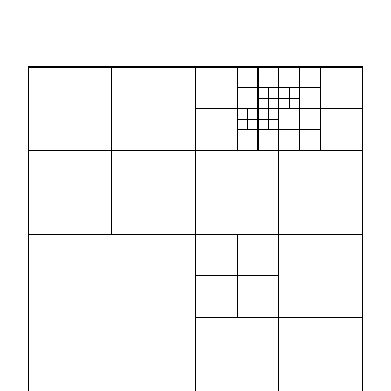
\begin{tikzpicture}[x={(.35\textwidth,0)},y={(0,.35\textwidth)}]
            % Three-dimensional versions
            \newrobustcmd{\drawthreedplus}[4]{\def\cx{#1} \def\cy{#2} \def\cz{#3} \def\s{#4} \drawthreedplushelper}
            \newrobustcmd{\drawthreedplushelper}[6]{;\draw (\cx+\s*#1/2,\cy+\s*#2/2,\cz+\s*#3/2) -- +(\s*#4,\s*#5,\s*#6); \draw (\cx+\s*#4/2,\cy+\s*#5/2,\cz+\s*#6/2) -- +(\s*#1,\s*#2,\s*#3);}
            \newrobustcmd{\threedrectpath}[7]{-- ++(#1*#2,#1*#3,#1*#4) -- ++(#1*#5,#1*#6,#1*#7) -- ++(-#1*#2,-#1*#3,-#1*#4) -- cycle}
            
            % Front side
            \draw (0,0,1) \threedrectpath{1} {1}{0}{0} {0}{1}{0};
            % Level 1
            \drawthreedplus{0}{0}{1} {1} {1}{0}{0} {0}{1}{0}
            % Level 2
            \drawthreedplus{1/2}{1/2}{1} {1/2} {1}{0}{0} {0}{1}{0}
            \drawthreedplus{1/2}{0/2}{1} {1/2} {1}{0}{0} {0}{1}{0}
            \drawthreedplus{0/2}{1/2}{1} {1/2} {1}{0}{0} {0}{1}{0}
            % Level 3
            \drawthreedplus{2/4}{3/4}{1} {1/4} {1}{0}{0} {0}{1}{0}
            \drawthreedplus{3/4}{3/4}{1} {1/4} {1}{0}{0} {0}{1}{0}
            \drawthreedplus{2/4}{1/4}{1} {1/4} {1}{0}{0} {0}{1}{0}
            % Level 4
            \drawthreedplus{5/8}{7/8}{1} {1/8} {1}{0}{0} {0}{1}{0}
            \drawthreedplus{6/8}{7/8}{1} {1/8} {1}{0}{0} {0}{1}{0}
            \drawthreedplus{5/8}{6/8}{1} {1/8} {1}{0}{0} {0}{1}{0}
            \drawthreedplus{6/8}{6/8}{1} {1/8} {1}{0}{0} {0}{1}{0}
            % Level 5
            \drawthreedplus{12/16}{14/16}{1} {1/16} {1}{0}{0} {0}{1}{0}
            \drawthreedplus{11/16}{14/16}{1} {1/16} {1}{0}{0} {0}{1}{0}
            \drawthreedplus{11/16}{13/16}{1} {1/16} {1}{0}{0} {0}{1}{0}
            \drawthreedplus{10/16}{13/16}{1} {1/16} {1}{0}{0} {0}{1}{0}
        \end{tikzpicture}
    }
    \subcaptionbox{\label{fig:octree}}[.575\textwidth]{
        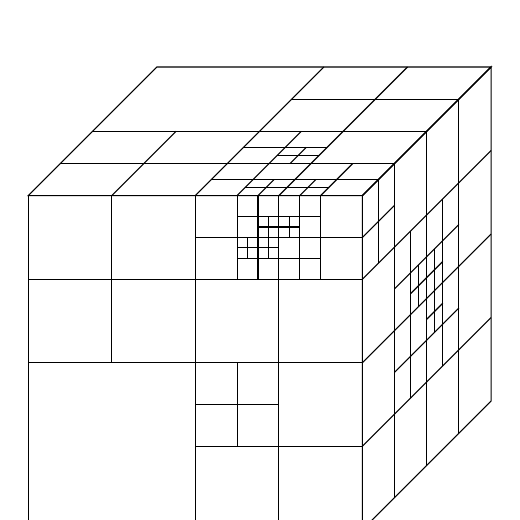
\begin{tikzpicture}[x={(.35\textwidth,0)},y={(0,.35\textwidth)},z={(-.385*.35\textwidth,-.385*.35\textwidth)}]
            % Two-dimensional versions
            %\newrobustcmd{\drawplus}[3]{;\draw (#1+#3/2,#2) -- (#1+#3/2,#2+#3); \draw (#1,#2+#3/2) -- (#1+#3,#2+#3/2);}
            %\newrobustcmd{\rectanglepath}[1]{-- ++(#1,0) -- ++(0,#1) -- ++(-#1,0) -- cycle}
            
            % Three-dimensional versions
            \newrobustcmd{\drawthreedplus}[4]{\def\cx{#1} \def\cy{#2} \def\cz{#3} \def\s{#4} \drawthreedplushelper}
            \newrobustcmd{\drawthreedplushelper}[6]{;\draw (\cx+\s*#1/2,\cy+\s*#2/2,\cz+\s*#3/2) -- +(\s*#4,\s*#5,\s*#6); \draw (\cx+\s*#4/2,\cy+\s*#5/2,\cz+\s*#6/2) -- +(\s*#1,\s*#2,\s*#3);}
            \newrobustcmd{\threedrectpath}[7]{-- ++(#1*#2,#1*#3,#1*#4) -- ++(#1*#5,#1*#6,#1*#7) -- ++(-#1*#2,-#1*#3,-#1*#4) -- cycle}
            
            % Front side
            \draw (0,0,1) \threedrectpath{1} {1}{0}{0} {0}{1}{0};
            % Level 1
            \drawthreedplus{0}{0}{1} {1} {1}{0}{0} {0}{1}{0}
            % Level 2
            \drawthreedplus{1/2}{1/2}{1} {1/2} {1}{0}{0} {0}{1}{0}
            \drawthreedplus{1/2}{0/2}{1} {1/2} {1}{0}{0} {0}{1}{0}
            \drawthreedplus{0/2}{1/2}{1} {1/2} {1}{0}{0} {0}{1}{0}
            % Level 3
            \drawthreedplus{2/4}{3/4}{1} {1/4} {1}{0}{0} {0}{1}{0}
            \drawthreedplus{3/4}{3/4}{1} {1/4} {1}{0}{0} {0}{1}{0}
            \drawthreedplus{2/4}{1/4}{1} {1/4} {1}{0}{0} {0}{1}{0}
            % Level 4
            \drawthreedplus{5/8}{7/8}{1} {1/8} {1}{0}{0} {0}{1}{0}
            \drawthreedplus{6/8}{7/8}{1} {1/8} {1}{0}{0} {0}{1}{0}
            \drawthreedplus{5/8}{6/8}{1} {1/8} {1}{0}{0} {0}{1}{0}
            \drawthreedplus{6/8}{6/8}{1} {1/8} {1}{0}{0} {0}{1}{0}
            % Level 5
            \drawthreedplus{12/16}{14/16}{1} {1/16} {1}{0}{0} {0}{1}{0}
            \drawthreedplus{11/16}{14/16}{1} {1/16} {1}{0}{0} {0}{1}{0}
            \drawthreedplus{11/16}{13/16}{1} {1/16} {1}{0}{0} {0}{1}{0}
            \drawthreedplus{10/16}{13/16}{1} {1/16} {1}{0}{0} {0}{1}{0}
            
            % Top side
            \draw (0,1,0) \threedrectpath{1} {1}{0}{0} {0}{0}{1};
            % Level 1
            \drawthreedplus{0}{1}{0} {1} {1}{0}{0} {0}{0}{1}
            % Level 2
            \drawthreedplus{0/2}{1}{1/2} {1/2} {1}{0}{0} {0}{0}{1}
            \drawthreedplus{1/2}{1}{1/2} {1/2} {1}{0}{0} {0}{0}{1}
            \drawthreedplus{1/2}{1}{0/2} {1/2} {1}{0}{0} {0}{0}{1}
            % Level 3
            \drawthreedplus{2/4}{1}{3/4} {1/4} {1}{0}{0} {0}{0}{1}
            \drawthreedplus{3/4}{1}{3/4} {1/4} {1}{0}{0} {0}{0}{1}
            \drawthreedplus{2/4}{1}{2/4} {1/4} {1}{0}{0} {0}{0}{1}
            % Level 4
            \drawthreedplus{5/8}{1}{7/8} {1/8} {1}{0}{0} {0}{0}{1}
            \drawthreedplus{6/8}{1}{7/8} {1/8} {1}{0}{0} {0}{0}{1}
            \drawthreedplus{5/8}{1}{5/8} {1/8} {1}{0}{0} {0}{0}{1}
            
            % Right side
            \draw (1,0,0) \threedrectpath{1} {0}{1}{0} {0}{0}{1};
            % Level 1
            \drawthreedplus{1}{0}{0} {1} {0}{1}{0} {0}{0}{1}
            % Level 2
            \drawthreedplus{1}{1/2}{1/2} {1/2} {0}{1}{0} {0}{0}{1}
            \drawthreedplus{1}{0/2}{1/2} {1/2} {0}{1}{0} {0}{0}{1}
            \drawthreedplus{1}{1/2}{0/2} {1/2} {0}{1}{0} {0}{0}{1}
            \drawthreedplus{1}{0/2}{0/2} {1/2} {0}{1}{0} {0}{0}{1}
            % Level 3
            \drawthreedplus{1}{3/4}{3/4} {1/4} {0}{1}{0} {0}{0}{1}
            \drawthreedplus{1}{2/4}{2/4} {1/4} {0}{1}{0} {0}{0}{1}
            \drawthreedplus{1}{2/4}{1/4} {1/4} {0}{1}{0} {0}{0}{1}
            \drawthreedplus{1}{1/4}{2/4} {1/4} {0}{1}{0} {0}{0}{1}
            \drawthreedplus{1}{1/4}{1/4} {1/4} {0}{1}{0} {0}{0}{1}
            % Level 4
            \drawthreedplus{1}{3/8}{3/8} {1/8} {0}{1}{0} {0}{0}{1}
            \drawthreedplus{1}{4/8}{3/8} {1/8} {0}{1}{0} {0}{0}{1}
            \drawthreedplus{1}{4/8}{4/8} {1/8} {0}{1}{0} {0}{0}{1}
        \end{tikzpicture}
    }
    \caption{\subrefp{fig:quadtree} A \quadtree used to partition twodimensional space. \subrefp{fig:octree} An \octree used to partition three-dimensional space. Note that an octree is essentially the same as a quadtree but is extended from two to three dimensions. In this illustration, only half of the surface of the octree is visible.}
    \label{fig:quadtree_and_octree}
\end{figure}

%\pgfmathsetseed{1}
%\foreach \col in {black,red,green,blue}
%{
%    \begin{tikzpicture}[x=10pt,y=10pt,ultra thick,baseline,line cap=round]
%    \coordinate (current point) at (0,0);
%    \coordinate (old velocity) at (0,0);
%    \coordinate (new velocity) at (rand,rand);
%    \foreach \i in {0,1,...,100}
%    {
%        \draw[\col!\i] (current point)
%        .. controls ++([scale=-1]old velocity) and
%        ++(new velocity) .. ++(rand,rand)
%        coordinate (current point);
%        \coordinate (old velocity) at (new velocity);
%        \coordinate (new velocity) at (rand,rand);
%    }
%    \end{tikzpicture}
%}

\section{Varying level of detail}

In \thisprojectwork, an octree has been used to partition the \idxs{computational}{domain} (the space in which the simulation will be performed) into the \cells required by the \FVM. Since only the \surface of the water is visible in the \simulation, the \idxsp{surface}{cell}{s} have been given a high \LOD; the \LOD then decreases at the water depth increases, staying a few \idxse{layer of}{cells}{layers of cells} a time on each \LOD, forming a \idxs{LOD}{layer} (a layer consisting of cells which all have the same \LOD, surrounded by cells with other \LODs).

Ideally, although not implemented in \thisprojectwork because of \itslimitedtime, the surface will have a higher \LOD where the \idxsp{surface}{detail}{s} are more important to the simulation, such as close to the \camera where they are more easily seen, and a lower \LOD far away from the camera where the cells take up little \idxse{screen}{space}{space on the screen}, or where they are out of the \FOV.

The total number of cells $N_{\text{t}}$ used in the simulationcan can be \approximated by an expression containing the thicknesses of the different LOD layers and the number of cells visible at the surface that belong to each \LOD accoring to

\begin{equation} \label{eq:number_of_cells_total_sum}
N_{\text{t}} \,=\, \sum_{i\,=\,0}^\infty N_{\text{s},i}\sum_{j\,=\,i}^\infty d_j\cdot 4^{-(j-i)},
\end{equation}

where $N_{\text{s},i}$ is the number of cells visible on the surface belonging to LOD layer $i$, and $d_j$ is the thickness in number of cells of LOD layer $j$, where LOD layer $0$ corresponds to the highest \LOD and an increasing LOD layer index corresponds to a lower \LOD. Different LOD layers can have different thickness; if this is the case, it will also be reflected in the simulation and waves with different wavelengths will be simulated with different \accuracy. In \thisprojectwork, all LOD layers have been given the same thickness, $d$. \eqref{eq:number_of_cells_total_sum} therefore turns into

\begin{equation} \label{eq:number_of_cells_total}
N_{\text{t}} \,=\, d\sum_{i\,=\,0}^\infty N_{\text{s},i}\sum_{k\,=\,0}^\infty 4^{-k} \,=\, d\,N_{\text{s}}\,\frac{1}{1-4^{-1}} \,=\, \frac{4}{3}\,d\,N_{\text{s}},
\end{equation}

where $k = j-i$ and $N_{\text{s}}$ is the total number of cells visible on the surface. We can therefore in this case conclude that

\begin{equation} \label{eq:number_of_cells_total_ordo}
N_{\text{t}} \,=\, O(N_{\text{s}}).
\end{equation}

Hence, the \idx{time step} for updating the \idxs{fluid}{flow} is roughly porportional to the number of \idxsp{surface}{cell}{s} $N_{\text{s}}$, but the simulation still catches all motion under the surface, with decaying \accuracy at increasing \idxsp{water}{depth}{s}.

\section{The differentiating problem}

\subsection{Perturbed cell interfaces method}

\subsection{Distributed velocities method}

\section{Multilevel acceleration}

\section{Spurious wave reflections at level transitions}
\chapter{Free Surface Modelling (FSM)}

There are both surface trackibng methods and surface capturing methods.

See also \textit{\href{http://physbam.stanford.edu/~fedkiw/papers/cam1998-17.pdf}{A Non-Oscillatory Eulerian Approach to Interfaces in Multimaterial Flows (The Ghost Fluid Method)}}

and \textit{\href{http://physbam.stanford.edu/~fedkiw/papers/stanford2002-07.pdf}{Robust Treatment of Interfaces for Fluid Flows and Computer Graphics}}

\begin{itemize}
    \item Lecture: \textit{\href{http://www.ims.nus.edu.sg/Programs/fluiddynamic/files/Lecture1-basics.pdf}{Moving Interface Problems: Methods \& Applications Tutorial Lecture I}}
\end{itemize}

\section{Level set method}

\subsection{Marching cubes}

\section{Volume of fluid method}

\begin{itemize}
    \item Reference: \textit{\href{http://pages.csam.montclair.edu/~yecko/icodes/HirtNichols_Surfer_JCP1981.pdf}{Volume of Fluid (VOF) Method for the Dynamics of Free Boundaries}}
    \item Comparsion: \textit{\href{http://capfluidicslit.mme.pdx.edu/reference/Numerics/Gopala_ChemEngJ2008_VOFMethodsFreeSurfaceFlow.pdf}{Volume of fluid methods for immiscible-fluid and free-surface flows}}
\end{itemize}

\subsection{VOF vs. Pseudo VOF}

\begin{itemize}
    \item Explanation: \textit{\href{http://www.flow3d.com/cfd-101/cfd-101-VOF.html}{VOF (Volume of Fluid) - What's in a Name?}}
\end{itemize}

\subsection{Interface reconstruction}
%\section{Internal alpha distribution}

\subsection{Smearing during advection}

\subsection{Geometric advection schemes}

\begin{itemize}
    \item A simple (at least so it seems) scheme: \textit{\href{http://www.lmm.jussieu.fr/~zaleski/nota02.pdf}{A geometrical area-preserving Volume-of-Fluid advection method}}
\end{itemize}

\subsection{Algebraic advection schemes}

\subsubsection{Convection Boundedness Criterion (CBC)}

\sloppy
\begin{itemize}
    \item Reference: \textit{Curvature-compensated Convective Transport: SMART a New Boundedness- Preserving Transport Algorithm}
    \item Extended Convective Boundedness Criterion (ECBC): \textit{Discussion on Numerical Stability and Boundedness of Convective Discretized Scheme}
    \item General Convective Boundedness Criterion (GCBC): \textit{\href{http://gr.xjtu.edu.cn:8080/upload/PUB.1673.4/Wei_NHT.pdf}{A New General Convective Boundedness Criterion}}
    \item \red{Convection Boundedness Criterion for arbitrarily unstructured meshes:} \textit{\href{http://powerlab.fsb.hr/ped/kturbo/openfoam/papers/GammaPaper.pdf}{High resolution NVD differencing scheme for arbitrarily unstructured meshes}}
\end{itemize}
\fussy

More:
\begin{itemize}
    \item Normalised Variable Diagram (NVD)
    \item \textit{\href{http://warminski.pollub.plwww.ptmts.org.pl/Waclaw-Koron-2-08.pdf}{Comparison of CICSAM and HRIC High-resolution Schemes for Interface Capturing}}
    \item \textit{\href{http://proceedings.fyper.com/eccomascfd2006/documents/85.pdf}{MODELING OF THE WAVE BREAKING WITH CICSAM AND HRIC HIGH-RESOLUTION SCHEMES}}
\end{itemize}

\subsubsection{Multidimensional Universal Limiter with Explicit Solution (MULES)}

References: \citep{Berberovi2009,Kissling2010}

See \textit{OpenFOAM-1.5.x/src/finiteVolume/fvMatrices/solvers/MULES/MULES.H} for details

See also \href{http://fds.duke.edu/db/aas/Physics/weller}{Henry R Weller, Professor Emeritus}

% Escape characters
%\& \% \$ \# \_ \{ \}
%\textasciitilde  = ~
%\textasciicircum = ^
%\textbackslash   = \

\begin{itemize}
    \item Described here: \textit{\href{http://link.libris.kb.se/sfxliub?sid=?url_ver=Z39.88-2004&rfr_id=info:sid/bibl.liu.se\%3Axerxes+\%28+PubMed+LiU\%29&rft.genre=article&rft_val_fmt=info\%3Aofi\%2Ffmt\%3Akev\%3Amtx\%3Ajournal&rft.issn=15393755&rft.date=2009&rft.jtitle=Phys+Rev+E+Stat+Nonlin+Soft+Matter+Phys&rft.volume=79&rft.issue=3+Pt+2&rft.spage=036306&rft.atitle=Drop+impact+onto+a+liquid+layer+of+finite+thickness+\%3A+dynamics+of+the+cavity+evolution+&rft.aulast=Berberovi\%C4\%87&rft.aufirst=Edin}{Drop impact onto a liquid layer of finite thickness: Dynamics of the cavity evolution}}
    \item An improvement for more than two phases: \textit{\href{http://www.mathematik.uni-ulm.de/numerik/staff/urban/reports/ECCOMASCFD2010paperfinal.pdf}{A Coupled Pressure Based Solution Algorithm Based on the Volume-Of-Fluid Approach for Two or More Immiscible Fluids}}
\end{itemize}

\subsubsection{SOLA-VOF}

\begin{itemize}
    \item Reference: \textit{\href{http://www.ewp.rpi.edu/hartford/~ernesto/Su2012/CFD/Readings/SOLA-VOF-1980-P1.pdf}{SOLA-VOF: A Solution Algorithm for Transient Fluid Flow with Multiple Free Boundaries}}
\end{itemize}

\subsubsection{Hyper-C flux limiter}

\begin{itemize}
    \item Reference: \textit{\href{http://www.water.tkk.fi/wr/kurssit/Yhd-12.112/TVD1.pdf}{The Ultimate Conservative Difference Scheme Applied to Unsteady One-Dimensional Advection}}
\end{itemize}

\paragraph{Floating mixed cells}

\begin{itemize}
    \item Remedy: \textit{\href{https://e-reports-ext.llnl.gov/pdf/245038.pdf}{A Simple Advection Scheme for Material Interface}}
\end{itemize}

\subsubsection{Compressive Interface Capturing Scheme for Arbitrary Meshes (CICSAM)}

\begin{itemize}
    \item Reference: \textit{\href{http://ac.els-cdn.com/S0021999199962769/1-s2.0-S0021999199962769-main.pdf?_tid=85161b57da5f4401e55c9d07495e24ea&acdnat=1336167249_a59e4f578adbacf3bff69936c48cdd57}{A Method for Capturing Sharp Fluid Interfaces on Arbitrary Meshes}}
    \item Also described in (by the same author): \textit{\href{http://powerlab.fsb.hr/ped/kturbo/OpenFOAM/docs/OnnoUbbinkPhD.pdf}{Numerical prediction of two fluid systems with sharp interfaces}}
    \item Test with different Courant numbers: \textit{\href{http://www.marin.nl/upload_mm/8/2/c/1807524470_1999999096_2007-ECCOMAS_HoekstraVazAbeilBunnik.pdf}{Free Surface Flow Modelling with Interface Capturing Techniques}}
    \item Improvement 1: \textit{\href{http://powerlab.fsb.hr/ped/kturbo/openfoam/docs/HenrikRuschePhD2002.pdf}{Computational Fluid Dynamics of Dispersed Two-Phase Flows at High Phase Fractions}}
\end{itemize}

\subsubsection{High Resolution Interface Capturing (HRIC) scheme}

\begin{itemize}
    \item Described here: \textit{\href{http://warminski.pollub.plwww.ptmts.org.pl/Waclaw-Koron-2-08.pdf}{Comparison of CICSAM and HRIC High-resolution Sche\-mes for Interface Capturing}}
\end{itemize}

\subsubsection{Switching Technique for Advection and Capturing of Surfaces scheme (STACS)}

\begin{itemize}
    \item Reference: \textit{\href{http://webfea-lb.fea.aub.edu.lb/cfd/pdfs/publications2/STACS-Complete.pdf}{Convective Schemes for Capturing Interfaces of Free-Surface Flows on Unstructured Grids}}
\end{itemize}

\subsubsection{Inter-Gamma Scheme}

\begin{itemize}
    \item Reference: \textit{\href{http://powerlab.fsb.hr/ped/kturbo/openfoam/docs/InterTrack.pdf}{Interface Tracking Capabilities of the Inter-Gamma Differencing Scheme}}
\end{itemize}

\subsubsection{Constrained Interpolation Profile (CIP) method}

%TODO: Used for advecting fluid interfaces?? At least apparently very good for simple advection.

\begin{itemize}
    \item Reference: \textit{\href{http://www.mech.titech.ac.jp/~ryuutai/paper/JCP2001CIPReviewYabe.pdf}{The Constrained Interpolation Profile Method for Multiphase Analysis}}
\end{itemize}

\subsection{Advection schemes for compressible water}

\begin{itemize}
    \item Remedy: Advect both water volume and total volume and then define alpha as the ration between them
\end{itemize}

\subsubsection{Fast Compressive Surface Capturing Formulation (FCSCF)}

\begin{itemize}
    \item Reference: \textit{\href{http://researchspace.csir.co.za/dspace/bitstream/10204/5282/1/Heyns_2011.pdf}{Free-Surface Modelling Technology for Compressible and Violent Flows}}
\end{itemize}

\section{Coupled Level Set/Volume of Fluid  method}

\begin{itemize}
    \item Reference: \textit{\href{http://pages.csam.montclair.edu/~yecko/icodes/SussmanPuckett_LevelSetVOF.pdf}{A Coupled Level Set and Volume-of-Fluid Method for Computing 3D and Axisymmetric Incompressible Two-Phase Flows}}
\end{itemize}
\chapter{Advection of properties}
\label{chap:advectionofproperties}

The choice of \idxs{advection}{scheme} depends entirely on the type of filed that is being exposed to advection and the necessary requirements that field puts on the advection scheme.

\section{Advection of smooth fields}

For a field with smooth changes and no sharp edges, which type the advection scheme is of is usually not that important, as long as it is stable and advects the field properly. Because of the low requirements, \idxsp{linear}{advection scheme}{s} are often used because of their simplicity and for the fact that linearity often brings a lot of benefits with it, for example the possibility to use \idxs{Fourier}{analysis} to study each frequency of the field that is exposed to advection independently of the other frequencies.

%\subsection{Stability of linear advection schemes}
\subsection{Stability and energy preservation}

For an advection scheme to be stable, no frequency, or eigenvector for an irregular grid, must be amplified, that is, any eigenvalue $\lambda_i$ of the $i$th eigenvector must have an absolute value less than or equal to one, i.e.\ $|\lambda_i| \leq 1$. When this requirement is not fulfilled, instability will occur, which is characterized by escalating oscillations and is usually the most evident for short wavelengths.

%\subsection{Smearing caused by linear advection schemes}

It is also often desired that the advection scheme damps the frequencies of the field as little as possible in order to preserve the energy in the field. Just like the amplifying that occurs for an instable advection scheme, damping is usually strongest for short wavelengths. The damping that occurs during advection is caused by the interpolation that is performed when moving the discretized field, and is often referred to as \smearing because of its low-pass filtering character. This causes an energy loss which is often undesired, even though it in many cases is considered a minor issue since it only affects the fine level details. Damping occurs whenever an eigenvalue $\lambda_i$ has an absolute value less than one, i.e.\ $|\lambda_i| < 1$.

\subsection{Error reduction for linear advection schemes}

A method that was originally intended to improve the quality of the \LS method, known as \BFECC, was first described in a publication by \citet{Dupont2003}. However, \BFECC can also be used to improve the energy preservation in any non-ideal, linear operator $A$ acting on a smooth field $\Phi$ (or a vector or any other object on which it makes sense to apply a linear operator), where A is an \approximation of an ideal (at least theoretically existing) operator $A^*$. This ideal operator is both stable and doesn't introduce damping. Let's assume that our goal is to improve the operator $A$ in such a way that the damping is reduced. \BFECC works under the circumstances that $A$ has a corresponding reverse operator $A'$ which is an \approximation of $(A^*)^{-1}$ and has an equal damping effect on the frequencies in the field as $A$, or more specifically, $A'$ has the same \eigenfunctions as $A$, with the corresponding eigenvalues
%
\begin{equation}
\lambda'_i \,=\, \overline{\lambda_i}, \,\forall\,i,
\end{equation}
%
where $\lambda'_i$ is the eigenvalue of the $i$th \eigenfunction of $A'$, and an overline denotes a complex conjugation. For a linear advection scheme, if $A$ is an operator that advects the field in a specific way, $A'$ is simply the operator that uses the same advection scheme as $A$ but that takes a field that has been advected by $A$ back to the position it came from.

In \BFECC, $\Phi$ is first updated forward in time, and then backwards to get another copy of the field, $\Phi_1$, such that $\Phi_1 = A'A\,\Phi$. If there would have been no numerical error, $A'$ would have been the inverse of $A$ and $\Phi$ and $\Phi_1$ would have been equal. The idea is to use the difference $\Phi_1-\Phi$ as information about the error, and use this information to compensate $\Phi$ before applying $A$. Since the error is introduced twice when calculating $\Phi_1$, a compensated variable $\Phi_2$ is calculated using only half of $\Phi_1-\Phi$, or
%
\begin{equation}
\Phi_2 \,=\, \Phi - \tfrac{1}{2}(\Phi_1 \,-\, \Phi).
\end{equation}
%
$A^*\Phi$ can then more accurately be \approximated as $A\,\Phi_2$, which in turn can be expanded to
%
\begin{equation}
\begin{array}{c}
A\,\Phi_2 \,=\, A\,\left(\Phi \,-\, \tfrac{1}{2}(\Phi_1 \,-\, \Phi)\right) \,=\, A\,\Phi \,-\, \tfrac{1}{2}(A\,A'A\,\Phi \,-\, A\,\Phi) \\
=\, A\,\left(\tfrac{3}{2} \,-\, \tfrac{1}{2}A'A\right)\,\Phi \,=\, \tilde{A}\,\Phi,
\end{array}
\end{equation}
%
where $\tilde{A}$ is defined as
%
\begin{equation} \label{eq:compensated_advection_operator}
\tilde{A} \,=\, A\,\left(\tfrac{3}{2} \,-\, \tfrac{1}{2}A'A\right)
\end{equation}
 %
and is an improved approximation of $A^*$. As can be seen, $\tilde{A}$ is the product of $A$ and a \polynomial of $A'A$, and the polynomial could if desired easily be extended with more terms as discussed in the end of this \levelname. Now, if we let this operator act on an \eigenfunction $\phi$, whose \eigenvalue is $\lambda$ when $A$ is acting on it and $\lambda' = \overline{\lambda}$ when $A'$ is acting on it, we see that 
%
\begin{equation}
\renewcommand*{\arraystretch}{1.5}
\begin{array}{c}
\displaystyle
\tilde{A}\,\phi \,=\, A\,\left(\tfrac{3}{2} \,-\, \tfrac{1}{2}A'A\right)\,\phi \,=\, \lambda\,\left(\tfrac{3}{2} \,-\, \tfrac{1}{2}\overline{\lambda}\lambda\right)\,\phi \\
\displaystyle =\, \frac{\lambda}{|\lambda|}\,\left(\tfrac{3}{2}\,|\lambda| \,-\, \tfrac{1}{2}|\lambda|^3\right)\,\phi \,=\, \tilde{\lambda}\,\phi,
\end{array}
\end{equation}
%
where $\tilde{\lambda} = \lambda/|\lambda|\,\left(\tfrac{3}{2}\,|\lambda| \,-\, \tfrac{1}{2}|\lambda|^3\right)$ is the eigenvalue of $\phi$ when $\tilde{A}$ is acting on it. If $|\lambda|$ is written as
%
\begin{equation}
|\lambda| \,=\, 1 - h, \quad h \leq 1
\end{equation}
%
where $h$ is a measure of the amount of damping introduced by $A$, we see that
%
\begin{equation}
\renewcommand*{\arraystretch}{1.5}
\begin{array}{c}
|\tilde{\lambda}| \,=\, \left|\tfrac{3}{2}\,|\lambda| \,-\, \tfrac{1}{2}|\lambda|^3\right| \,=\, \left|\tfrac{3}{2}\,(1-h) \,-\, \tfrac{1}{2}(1-h)^3\right| \\
=\, \left|\tfrac{3}{2}-\tfrac{3}{2}\,h \,-\, \tfrac{1}{2} + \tfrac{3}{2}\,h - \tfrac{3}{2}\,h^2 + \tfrac{1}{2}\,h^3\right| \,=\, \left|1 - \displaystyle\frac{3\,h^2 - 1\,h^3}{2}\right|.
\end{array}
\end{equation}

The damping introduced by $\tilde{A}$ is given by $\tilde{h} = 1 - |\tilde{\lambda}|$. If we assume that possible instabilities in $A$ are small, which means that $-h \ll 1$ if $h < 0$, and consider the fact that $h \leq 1$, $\tilde{h}$ can be expanded to
%
\begin{equation}
\tilde{h} \,=\, 1 - |\tilde{\lambda}| \,=\, 1 - \frac{|\lambda|}{|\lambda|}\left|1 - \displaystyle\frac{3\,h^2 - 1\,h^3}{2}\right| \,=\, \displaystyle\frac{3\,h^2 - 1\,h^3}{2} \,=\, O(h^2),
\end{equation}
%
and we see that the damping introduced by $\tilde{A}$ is of second order if we consider the damping introduced by $A$ to be of first order. We can also notice that if $A$ is unstable, which means that $h < 0$ (although still very small), $\tilde{h}$ will still be positive, which means that $\tilde{A}$ is stable. \BFECC will therefore both heavily reduce damping as well as fix small instabilities in $A$.

Similar schemes of even higher order can be obtained by extending the \polynomial that $\tilde{A}$ is partially composed of with even more terms of type $(A'A)^n$. Since we desire that $\tilde{\lambda} = \lambda/|\lambda|$, we require that the polynomial will result in a division by $|\lambda|$ when acting on $\phi$. This result is \approximated if we let the polynomial be an approximation of $1/\sqrt{A'A}$. The polynomial can therefore be expressed as a \idxs{Taylor}{polynomial} of $1/\sqrt{A'A}$ centered around the point $A'A = 1$. The Taylor polynomial in turn is given by the first terms of the \idxs{binomial}{series} of $(1+x)^{-\frac{1}{2}}$, where $x = A'A - 1$. All these schemes will be stable as long as $A$ is stable, and all schemes with even order will also stabilize the advection process if $A$ contains instabilities that are small enough.

Another approach to increase the order of the advection scheme is to apply \BFECC multiple times to improve the already improved approximation of $A^*$, each time doubling the order of the scheme, but also tripling the number of times $A$ and $A'$ has to be applied. This method is more bulletproof than the method using a Taylor polynomial as it theoretically can stabilize advection schemes with eigenvalues whose absolute values are up to (but less than) $\sqrt{5}$, while the stabilizing abilities of the method using a Taylor polynomial decreases the higher the order of the method becomes. On the other hand, it faster becomes slow when the order of the method increases, as it needs to use $A$ and $A'$\ \ $3^n$ times to obtain the order $2^n$, where $n$ is an integer, while the method using a Taylor polynomial only needs to use $A$ and $A'$\ \ $2\cdot 2^n - 1$ times to obtain the same order of the value $\tilde{h}$ used to measure the damping introduced by $\tilde{A}$ on $\phi$.

\section{Advection of the phase fraction field}

\label{sec:advection_of_phase_fraction}

In contrast to smooth fields, the phase fraction field $\alpha$ is supposed to be either 0 or 1 and have just a very thin region in which the transition between 0 and 1 takes place, i.e. a region in which $0 < \alpha < 1$. When advecting this field, three things are important:

\begin{enumerate}
\item That the mass is conserved, which corresponds to the conservation of $\alpha$,
\item That the field stays bound between 0 and 1, and
\item That the interface stays sharp and doesn't become thicker and thicker.
\end{enumerate}

\subsection{Geometric advection schemes}
\label{sec:geometric_advection_schemes}

\idxse{geometric}{advection scheme}{Geometric advection schemes} work by constructing a geometry for the surface from the discretized \idxs{phase fraction}{field}, and by using the generated geometry to calculate the fluxes between each adjacent pair of cells.

One of the most well known and common geometric advection schemes is \PLIC, which is also one of the advection schemes that introduces the least error. However, it comes at the cost of algorithmic complexity, especially in three-dimensional situations, where the tracking and reconstruction of free surfaces remains complex \citep{Ingram2009}.

Tracking of the free surface tends to be somewhat complex when using a geometric advection scheme. For example, in the two-dimensional case, a naive approach will lead to that volumes in cell corners may be fluxed twice --- once to each adjacent cell --- since there are two cells adjacent to each corner volume. In the three-dimensional case, a naive approach will lead to that edge volumes may be fluxed twice. Corner volumes may even be fluxed thrice since there are three cells adjacent to each corner volume, which makes the three-dimensional case even more complex that the two-dimensional.

This easily leads to unboundedness, as the amount of one phase that is fluxed from a cell during one time step may be larger than what is currently in the cell. Special concern must therefore be taken to the edge and corner volumes in order to prevent fluid from being fluxed to more than one other cell \citep{Rider1997}.

An alternative approach that avoids the complexity mentioned above is described by \citet{Aulisa2003}, where the phase fraction field is fluxed first in the x-direction and then in the y-direction, thus only requiring that each part of the cell that is fluxed, is fluxed to one cell at a time. However, this method is non-symmetric, as it is dependent on in which order the phase fraction field is fluxed in the different dimensions; this fact is discussed further by \citet{Ubbink1999}, although this time the issue is discussed for an \idxs{algebraic}{advection scheme} --- \CICSAM.

\subsection{Algebraic advection schemes}

As opposed to geometric advection schemes, a geometric representation of the surface is never created in an \idxs{algebraic}{advection scheme}. This usually makes these methods a lot simpler than most geometric advection schemes, and the reduced complexity may lead to a performance boost. In this thesis work, an algebraic advection scheme known as \idxs{Hyper-C}{flux limiter}, which was described by \citet{Leonard1988,Leonard1991} and which is optimal for \idx{one-dimensional}, \idxs{incompressible}{flow}, has been used in a form that has been modified to cope with \idxs{compressible}{flow}.

There exist other algebraic advection schemes that more suitable for multidimensioal incompressible flow, like \CICSAM, which was first described by \citet{Ubbink1999}, and \STACS, which was probably first described at earliest in 2003 \citep{Darwish}. The Hyper-C flux limiter, \CICSAM and \STACS are all derived from something known as the \CBC which is a criterion that --- if followed --- guarantees that the advected field stays bounded.

Furthermore, the \MULES method is also designed for multidimensional incompressible flow, but doesn't build on the \CBC. \MULES was designed for the \idxs{open}{source} software \idx{OpenFOAM} and has after its implementation been described by others than the original authors of the algorithm, for example by \citet{Berberovi2009}. It has also been improved to cope with more than two phases \citep{Kissling2010}, since that wasn't handled very well by the original formulation.

%\subsubsection{Algebraic advection schemes for compressible flows}

However, although \CICSAM, \STACS and \MULES are also designed for and work well for incompressible flow, they would have to be modified to cope with compressible flow. This can often be achieved by advecting \idxsp{volume}{fraction}{s} of both phases separately, and by defining $\alpha$ as the quotient of the volume fraction for one of the phases and the sum of the volume fractions for both phases, instead of simply as the volume fraction for one of the phases. This guarantees that $\alpha$ is equal to either 0 or 1 for a cell that contains only one phase. This problem is also discussed by \citet{Heyns2011}.

\chapter{Method summary}

To make things clear, this is a short summary of all methods that have been used in \thisprojectwork.

The \FVM on a \idxs{stagered}{grid} has been used. The \PDEs that have been solved are the \idxs{Euler}{equations} and the flow has been considered to be \idxse{compressible}{flow}{compressible}.

The grid has been modeled with an \octree. The \LOD of the \idxsp{water surface}{cell}{s}\indexs{surface}{cell} depends on how visually important they are, and the \LOD of the \idxsp{bulk}{cell}{s} decreases the further down under the surface the cells are located. This ensures that the total number $N_t$ of cells used in the simulation is roughly proportional to the number $N_s$ of cells visible on the surface according to \eqref{eq:number_of_cells_total_ordo}.

The interface has been modeled using the \VOF method and the \idxs{advection}{scheme} used for transporting the \idxs{$\alpha$}{field} is a variant of the \idxs{Hyper-C}{flux limiter}\index{limiter!Hyper-C flux limiter|see{Hyper-C flux limiter}} that has been modified especially for compressible flow.

The region over the \idxs{water}{surface} is assumed to be \air. Initially, only cells that are at least partly filled with water are added to the octree, in order to save \idxs{computational}{power} (and since there would basically be an infinite number of air cells if they would have been represented). In order for the advection scheme to work properly, all cells with at least some water in them, i.e. $\alpha > 0$, also have to have neighbor cells in all directions the water can be advected, so whenever $\alpha$ for one cell goes from $\alpha = 0$ to $\alpha > 0$, all surfaces of the cell that don't border to another cell or to a \idxs{solid}{boundary} are found and cells with $\alpha = 0$ are created adjacent to those surfaces. This also happens automatically for all cells in the beginning of the simulations when cells initially get filled with water.

\part{Analysis}

\chapter{Results}

Whenever a cell with $\alpha = 0$ doesn't border to any cell with $\alpha > 0$, it is not needed any longer.

The idea was to remove them, although this feature was never implemented. Although the advection scheme that is used is ideal in \idxs{one}{dimension}\index{dimensions!one|see{one dimension}}, it proved to smear the \idxs{$\alpha$}{field} out somewhat in \idxse{two}{dimensions}{two} and \idxs{three}{dimensions}, making the interface between water and vacuum become thicker and thicker, which affects both the \idxs{simulation}{quality}, since the surface becomes less and less well-defined as the simulation goes on, as well as the \preformance of the \idxs{numerical}{method} since it will have to consider more and more cells as the interface gets thicker and thicker. Another advection scheme that maybe could remedy this problem is \MULES, described in \citep{Berberovi2009} and further developed to for better handling of more than two phases in \citep{Kissling2010}, although it would have to be modified to cope with compressible flow.

\HRule

% Pros:

The program that was developed could successfully simulate water and air and keep the two phases separated, with a region of cells containing a mix of both water and air in between. Pressure waves could be propagates in the bulks of the fluids, and gravity waves propagating on the surface in the interface between the water and the air were successfully be simulated.

% Cons:

The method chosen to simulate water waves in realtime, which was the \FVM on an \octree datastructure together with the \VOF, proved to be quite advanced and difficult to implemented properly within the time frame for \thismasterthesiswork, which was \masterthesisworktime. The simulations suffered from numerous problems for which there wasn't enough time to implement any remedy. Here is a list of issues that the simulation implementation from:

% although there would most likely have been several ways to fix all of them in.

%The limitation of the Courant number is a big problem, as it prevents the simulation from taking as large time steps as it would have to; this could maybe be remedied by switching from explicit to implicit methods. On the other hand, it can now manage to propagate surface waves.

\begin{itemize}
    \item Vacuum could suddenly occur in the air regions, causing a numerical instability that would spread through the entire simulation domain and "eat up" the contents of all other cells.
    
    %\item Vacuum could suddenly occur in the air regions, causing velocities to go to infinity. With constant time step, this lead to numerical instabilities, while with an adaptive time step, this lead to that the simulation went slower and slower the closer the content of a cell came to vacuum and the higher the velocity went, and it would eventually freeze completely. In any case, one of the cells would eventually lose all its content, which would start a numerical instability that would spread like wildfire and "eat up" all the rest of the air and water in the entire simulation domain. This issue did't occur until the simulation had been running for a while and was not a bug, but a result of the way the equations were solved.
    
    \item The simulation speed was extremely low. % Even though the tests carried out during the development of the program were only held in two dimensions, and thus heavily reduced the number of cells to be processed in each time step, the simulation still went many times slower than realt-time speed. This was partly due to the fact that no optimization or paralellization of the code was made, and partly due to the fact that the time step was restricted by the \CFL condition, which forced the time step to be as low as 0.3~ms which corresponds to a \idx{frame rate} of 3333~\FPS, while the frame rate only needed to be at \flightsimulatorfps~\FPS.
    
    \item There were problems with keeping the interface intact. % Unlike linear advection schemes, like \UPWIND, the \idx{Hyper-C} advection scheme, of which a variant was implemented in \thisprojectwork, is supposed to keep the interface compressed. However, the interface was not kept compressed and water was churned up in the air and formed something that closest resembled a kind of mist, which is very non-ideal for several reasons. First, visualization becomes more difficult, since the thicker the interface is the more difficult it is to know where the surface is located. Second, all cells that contain at least some water have to be processed, which means that a thick interface will decrease the simulation speed significantly. Third, a thick interface is a bad \approximation of a real surface interface, whose thickness is almost zero, and numerical errors will be introduced as a result of that.
    
    %It is unknown whether the the fact that the interface grew so large is a property of the Hyper-C advection scheme, if it was because the Hyper-C advection scheme was implemented incorrectly, or just because it is difficult to gereralize these kinds of interface compressing advection schemes to support complessible flows. It is also unknown whether the thickness of the interface would grow arbitrarily large if the simulation would continue to go on without being subject to numerical instability, or if the thickness would eventually stabilize at a certain level.
\end{itemize}

\HRule

\begin{itemize}
    \item Not just the water was simulated, but also the air. % This is a fact that also meant that the simulation domain needed also to have a boundary in the air. This introduced the additional problem of choosing where this boundary should be located, why it should be located at that place, and what boundary conditions it should have. The fact that the air was also simulated meant that a lot of more cells had to be processed each time step than if only the water would have been simulated, which had a significant impact on the simulation speed.
    
    \item The simulation used explicit numerical methods, which meant that it was limited by the \CFL condition. % This meant that the Courant number couldn't exceed one, which limited the time step to a very small value which made it practically impossible to come even near real time speed.
    
    \item Fluid--structure interaction was not implemnted. % This is necessary in order to be able to simulate wakes after ships or in order for waves to make ships rock forth and back.
\end{itemize}


\HRule

\chapter{Discussion}

\section{Conservation laws}

\begin{itemize}
    \item Mass
    \item Energy
    \item (d/d$t$)\,Momentum $-$ Force = 0
    \item Angular momentum
    \item (d/d$t$)\,(Center of mass) $-$ Momentum = 0
\end{itemize}

\section{Already existing software}

\begin{itemize}
    \item OpenFOAM (\red{FOAM, see} \textit{\href{http://powerlab.fsb.hr/ped/kturbo/openfoam/docs/foam.pdf}{A tensorial approach to computational continuum mechanics using object-oriented techniques}})
\end{itemize}

Reasons to use them: They have been tried out and they work, maybe not exactly for these purtposes, though. It saves time to use them instead of having to develop your own software. Reasons for developing you own software: You get full control of what you are doing, so you can adapt the software after your needs. You can approximate and simplify the things that are usually important but not for this purpose, so you can optimize the code for your purpose. You don't have to pay for any license; this otherwise have a tendency to become really expensive for a large company.

\section{Other methods to use}

For realtime simulation of surface waves in large bodies of water, where non-linear phenomena are not of any significant importance, the best method to use, considering both implementation time and simulation quality, is probably spectral methods.

\chapter{Improvements}

Except from these problems with the implementation that was made, it would need a lot of improvements in order to be applicable in a real-time flight simulator.

\section{Adapdive Meshing}

LODs that adapt to the camera placement and the Field of View (FOV)/Viewing frustum in order to limit the number of cells needed in the FVM

\section{Fluid--Structure Interactin}

see e.g.:

\begin{itemize}
    \item \textit{\href{http://physbam.stanford.edu/~fedkiw/papers/stanford2010-04.pdf}{Numerically Stable Fluid-Structure Interactions Between Compressible Flow and Solid Structures}}
    \item \textit{\href{http://efdl.as.ntu.edu.tw/research/papers/JCP03GCIBM.pdf}{A ghost-cell immersed boundary method for flow in complex geometry}}
    \item \textit{\href{http://www.cs.columbia.edu/~batty/papers/Batty07.pdf}{A Fast Variational Framework for Accurate Solid-Fluid Coupling}} (solid fraction, non-stick to walls)
\end{itemize}

\subsection{Immersed Boundary Method}

\begin{itemize}
    \item Reference: \textit{\href{http://www4.ncsu.edu/~zhilin/TEACHING/MA798Z/Peskin1.pdf}{The immersed boundary method}}
    \item For compressible flow: \textit{\href{http://www.cecs.wright.edu/~haibo.dong/wp-content/themes/publications/IBM_JCP_2007.pdf}{A sharp interface immersed boundary method for compressible viscous flows}}
\end{itemize}

\subsection{Volume of Solid Method (VOS)}

\begin{itemize}
    \item Reference: \textit{The simulation of fluid-rigid body interaction}
    \item Described in \textit{Numerical Modeling of Deforming Bubble Transport Related to Cavitating Hydraulic Turbines}
\end{itemize}

\subsection{Rigid Fluid method}

\begin{itemize}
    \item Reference: \textit{\href{http://www.amath.unc.edu/Faculty/mucha/Reprints/siggraph04.pdf}{Rigid Fluid: Animating the Interplay Between Rigid Bodies and Fluid}}
\end{itemize}

\subsection{Rotation of rigid bodies}

See \textit{\href{http://en.wikipedia.org/wiki/Euler\%27s_equations_\%28rigid_body_dynamics\%29}{Euler's equations (rigid body dynamics)}}

\section{Parallellization}

See e.g. \textit{\href{http://gfs.sourceforge.net/papers/agbaglah2011.pdf}{Parallel simulation of multiphase flows using octree adaptivity and the volume-of-fluid method}}

\subsection{Space filling curves}

See e.g. \textit{\href{http://j.teresco.org/research/publications/octpart02/octpart02.pdf}{Dynamic Octree Load Balancing Using Space-Filling Curves}}

and \textit{\href{http://downloads.isrn.com/journals/appmath/2012/246491.pdf}{Parallel Adaptive Mesh Refinement Combined with Additive Multigrid for the Efficient Solution of the Poisson Equation}}

\section{Implicit Time-Stepping}

\SIMPLE (although not co,pletely implicit (?))

Switch from explicit to implicit methods to allow arbitrarily large time steps

\section{Visualization}

\subsection{Marching Cubes}

\subsection{Surface shininess}

Shading/reflection (increased reflection spreading for increased height = shininess as a function of the part of the spectrum that contains the supressed high-frequency waves)

\section{Local-time stepping}

Very dubious technique as you can make the method allow large time steps. (see below)

\section{Large time steps}

See e.g. \textit{\href{http://www.dgp.toronto.edu/people/stam/reality/Research/pdf/ns.pdf}{Stable fluids}}

\section{Remedy for regions with high Courant number}

\section{Perfectly matched layers}

Avoiding spurious reflections at LOD transitions (Absorbing boundary conditions, Perfectly Matched Layers)

See e.g. \textit{\href{http://liu.diva-portal.org/smash/get/diva2:359805/FULLTEXT01}{Memory Efficient Methods for Eulerian Free Surface Fluid Animation}}

\section{Wind waves}

Wind waves (wave generation)

\subsection{Spectral methods}

\subsection{Air-water interaction}

\section{Visual effects}

\subsection{Splash and foam}

(See \textit{\href{http://en.wikipedia.org/wiki/Sea_foam}{Wikipedia -- Sea foam}} or search for \textit{protein skimming} or \textit{foam fractionation})

Implemented in \textit{\href{http://nguyendangbinh.org/Proceedings/Eurographics/2003/cgf/volume22/issue3/paper127/paper127.pdf}{Realistic Animation of Fluid with Splash and Foam}}

which references \textit{\href{http://citeseerx.ist.psu.edu/viewdoc/download?doi=10.1.1.4.6262&rep=rep1&type=pdf}{Rendering Natura lWaters}}

which in turn is based on work presented in the book \textit{\href{http://books.google.se/books?id=xuwFz1bPTHgC}{Oceanic Whitecaps: Their Role in Air-Sea Exchange Processes}} by E. C. Monahan and G. MacNiocaill.

See also \textit{\href{http://www.ias.ac.in/jess/sep2002/Ps18.pdf}{Oceanic whitecaps: Sea surface features detectable via satellite that are indicators of the magnitude of the air-sea gas transfer coefficient}} (also by  E. C. Monahan)

\section{Sharpening of various advected fields}

\subsection{Backward Error Compensation and Forward Error Correction}

\begin{itemize}
    \item Reference: \textit{\href{http://smartech.gatech.edu/xmlui/bitstream/handle/1853/29473/2002-389.pdf}{Back and forth error compensation and correction methods for removing errors induced by uneven gradients of the level set function}}
    \item Applied to the velocity field and images: \textit{\href{http://www.gvu.gatech.edu/~jarek/papers/FlowFixer.pdf}{FlowFixer: Using BFECC for Fluid Simulation}}
\end{itemize}

\section{Various optimizations}

* Pure code optimizations
* Local time stepping (dibious improvement)

\chapter{Conclusions}

The FVM on octrees with FSM (free surface modelling) is an advanced method and takes a long time to implement, probably a few years (wor at least much longer than half a year) to make it ideal/perfect for the aim/scope/purposes of this master thesis work. Probably not the most suitable method there is today for this master thesis work even after all the programming and development has been done since it requires much computational power to be satisfactory. Spectral methods are probably a better way and have even been implemented for purposes like these. But maybe this method would be ideal in the future, since the computation load is basically the only bottleneck of the method when it has been fully implemented. When that day comes, it will have the ability to run in real time and it will outclass every other method that doesn't simulate the water "for real", since they will always miss out on certain effects that they are not able to simulate. The FVM is simply the best mathematical model (that it's still possible to implement on a computer) there is when it comes to actually describing water waves, not necessarily when it comes to simulation speed. Besides, the method used in \thisprojectwork runs in the same time complexity as the fastest of the other methods.

\section{Difficulties and drawbacks with the method}

Difficulties:
\begin{itemize}
    \item Dynamical creation/termination of surface cells and determination of properties in new cells
    \item High Courant numbers
    \item High speeds of sound (remedied in \textit{\href{http://physbam.stanford.edu/~kwatra/papers/compressible_semi_implicit/compressible_semi_implicit.pdf}{A method for avoiding the acoustic time step restriction in compressible flow}})
    \item Keeping a sharp interface
    \item Making it work in realtime
\end{itemize}
\part{Appendices}
\appendix

\chapter{Algorithms and data structures}
\label{apdx:algorithmsanddatastructures}

\section{The octree}

\begin{figure}
    \centering
    \begin{tikzpicture}[x={(.35\textwidth,0)},y={(0,.35\textwidth)}]
    \def\@offset{.1}
    
    % The cells
    \draw (0,0) \squarepath{1};
    \drawplus{0}{0}{1}
    \draw (0.25,0.25) node{0};
    \draw (0.75,0.25) node{1};
    \draw (0.25,0.75) node{2};
    \draw (0.75,0.75) node{3};
    
    % The 0th index axes
    \draw[->] (0,-\@offset) -- (1,-\@offset);
    \draw (1+\@offset,-\@offset) node{$i_0$};
    \draw (.25,-2*\@offset) node{0};
    \draw (.75,-2*\@offset) node{1};
    
    % The 1th index axes
    \draw[->] (-\@offset,0) -- (-\@offset,1);
    \draw (-\@offset,1+\@offset) node{$i_1$};
    \draw (-2*\@offset,.25) node{0};
    \draw (-2*\@offset,.75) node{1};
    \end{tikzpicture}
    \caption{A parent cell with four child cells. The numbers written inside of the child cells are their corresponding indexes in their panet's child array.}
    \label{fig:octree_child_indexes}
\end{figure}

\begin{figure}
    \centering
    \subcaptionbox{\label{fig:octree_child_array_example_layout}}[.415\textwidth]{
        \begin{tikzpicture}[x={(.35\textwidth,0)},y={(0,.35\textwidth)}]
        % The cells
        % Level 0
        \draw (0,0) \squarepath{1};
        
        \drawplus{0}{0}{1}
        % Level 1
        \drawplus{0}{0}{1}
        \draw[pattern=north east lines] (0.5,0.5) \squarepath{0.5};
        % Level 2
        \drawplus{0.5}{0}{0.5}
        \draw[pattern=north east lines] (0.75,0.25) \squarepath{0.25};
        \end{tikzpicture}
    }
    \subcaptionbox{\label{fig:octree_child_array_example_data}}[.415\textwidth]{
        \pgfmathsetmacro{\wdbox}{.02\textwidth}
        \tikzset{
            >= stealth,
            every picture/.style={thick},
            %every picture/.style={ultra thick},
            every node/.style={anchor=north},
            %null/.style={\path (0,0) -- +(0,.65em) node {$\emptyset$};},
            octree/.style={draw,fill=white!100!black,minimum size=2*\wdbox-\pgflinewidth,scale=1},
            octcell/.style={draw,fill=white!100!black,minimum size=4*\wdbox-\pgflinewidth,scale=1},
            array/.style={%
                draw,
                fill=white!90!black,
                inner sep=0,
                %rounded corners,
                rectangle,
                rectangle split,
                rectangle split parts=4,
                rectangle split horizontal,
                rectangle split every empty part={},
                rectangle split empty part width=2*\wdbox-\pgflinewidth,
                rectangle split empty part height=2*\wdbox-\pgflinewidth,
                rectangle split ignore empty parts=false,
                append after command={%
                    \pgfextra{\let\mainnode=\tikzlastnode} 
                    coordinate (c0 \mainnode) at ($(\mainnode.west)!0.5!(\mainnode.one split)$)
                    coordinate (c1 \mainnode) at ($(\mainnode.west)!1.5!(\mainnode.one split)$)
                    coordinate (c2 \mainnode) at ($(\mainnode.west)!2.5!(\mainnode.one split)$)
                    coordinate (c3 \mainnode) at ($(\mainnode.west)!3.5!(\mainnode.one split)$)
                }
            }
        }
        \begin{tikzpicture}[x=\wdbox,y=\wdbox]
        \node[octree] (0) {};
        \draw[->] (0.center)  -- +( 0,-4) node[octcell]  (1)  {};
        %\node[octcell] (1) {};
        \draw[->] (1.center)  -- +( 0,-4) node[array]  (2)  {};
        \draw[->] (c0 2)      -- +(-6,-4) node[octcell] (3)  {};
        \draw[->] (c1 2)      -- +(-2,-4) node[octcell] (4)  {};
        \draw[->] (c2 2)      -- +(+2,-4) node[octcell] (5)  {};
        %\draw[->] (c3 2)      -- +(+6,-4) node         (6)  {}; \path (6) -- +(0,.65em) node {$\emptyset$};
        \path (c3 2) -- +(0,.75em) node {$\emptyset$};
        %\draw[->] (3.center)  -- +( 0,-4) node         (7)  {$\emptyset$};
        \path (3.center) -- +(0,.75em) node {$\emptyset$};
        \draw[->] (4.center)  -- +( 0,-4) node[array]  (8)  {};
        %\draw[->] (5.center)  -- +( 0,-4) node         (9)  {$\emptyset$};
        \path (5.center) -- +(0,.75em) node {$\emptyset$};
        \draw[->] (c0 8)      -- +(-4,-4) node[octcell] (10) {};
        \draw[->] (c1 8)      -- +(-0,-4) node[octcell] (11) {};
        \draw[->] (c2 8)      -- +(+4,-4) node[octcell] (12) {};
        %\draw[->] (c3 8)      -- +(+8,-4) node         (13) {$\emptyset$};
        %\draw[->] (10.center) -- +( 0,-4) node         (14) {$\emptyset$};
        %\draw[->] (11.center) -- +( 0,-4) node         (15) {$\emptyset$};
        %\draw[->] (12.center) -- +( 0,-4) node         (16) {$\emptyset$};
        \path (c3 8) -- +(0,.75em) node {$\emptyset$};
        \path (10.center) -- +(0,.75em) node {$\emptyset$};
        \path (11.center) -- +(0,.75em) node {$\emptyset$};
        \path (12.center) -- +(0,.75em) node {$\emptyset$};
        %\draw (0,1)--(0,1);
        \end{tikzpicture}
    }
    \caption{An octree configuration. Note that the term octree here refers to a $D$-dimensional generalization of an octree, and that these images depict a 2-dimensional version for simplicity. \subrefp{fig:octree_child_array_example_layout} The spatial layout of the octree. A striped square denotes a non-existing cell on that location. \subrefp{fig:octree_child_array_example_data} The internal data representation of the octree. The small, white square is the tree object, the large, white squares are cell objects, the gray rectangles split into $2^D$ (four in this illustration) parts are child arrays and the arrows are pointers. A $\emptyset$ sign denotes a \NULL pointer, i.e. a pointer whose value is zero, which codes for a non-existing cell or child array.}
    \label{fig:octree_child_array_example}
\end{figure}

Although an octree is a \idxs{three-dimensional}{data structure} and a tree in which all \idxsp{parent}{node}{s} has exactly eight \idxsp{child}{node}{s}, the octree implementation used in \thisprojectwork is a generalized version of an octree and works for any number $d$ of \dimensions and where each \idxs{parent}{cell} (a \cell is a \node with a physical representation) has between 1 and $2^d$ \idxsp{child}{node}{s}. 

The \octree itself just consists of a \pointer to the \idxs{root}{cell}\indexs{root}{node} and a few \methods for manipulating the \cells in the tree. If the octree is empty, the value of the pointer is \NULL.

Each cell in the tree then contains a pointer to a \idxs{child}{array}, which is an array of pointers to the child cells. If a cell is a \idxs{leaf}{cell}, it doesn't have any children and the value of the pointer to the child array is \NULL. If the cell does have children, the pointer points to an actual array consisting of \numchildren pointers to \idxsp{octree}{cell}{s}. If such a pointer is \NULL, it means that the corresponding child doesn't exist; otherwise, the pointer points to the child cell. The index $i$ of an array element corresponds to the position of the child cell relative the parent cell according to

\begin{equation} \label{eq:child_node_index_general}
i \,=\, \sum_{j=0}^{d-1} \,2^j\,i_j,
\end{equation}

where $i_j$ is an index that is either 0 or 1 and corresponds to the position of the child cell relative to the parent cell along $\normvec{e}_j$, as shown in \figref{fig:octree_child_indexes}. Just as an example, in three dimensions \eqref{eq:child_node_index_general} reduces to

\begin{equation} \label{eq:child_node_index_three_dimensions}
i \,=\, i_0 + 2\,i_1 + 4\,i_2.
\end{equation}

This structure is illustrated in \figref{fig:octree_child_array_example}.

\section{Neighbor connections}

In \thisprojectwork, \idxse{neighbor}{cell}{neighboring cells} are physically linked to each other, and each cell contains five \idxsp{doubly linked}{list}{s}\indexs{doubly}{lined list} whit \idxse{neighbor}{connection}{connections} to neighbor cells. The reason why doubly linked lists are used to store the connections is because their content is constantly changing because of the dynamic \idxs{water}{surface} and the dynamically changing \LODs, which both cause the grid to constantly have to \remesh itself and update its neighbors, and any nieghbor connection can have to be removed at any moment. The five doubly linked lists contains connections to

\begin{enumerate}
    \item \idxse{leaf}{cell}{Leaf cells} at the next lower \LOD,
    \item \idxse{parent}{cell}{Parent cells} at the next lower \LOD,
    \item Leaf cells with at the same \LOD,
    \item Parent cells with at the same \LOD, and
    \item Cells at the next higher \LOD
\end{enumerate}

respectively. The reason connections both to leaf cells and to parent cells are stored is because it was originally planned to use the \idxs{multigrid}{method} for solving the \idxs{pressure}{Poisson equation} that needs to be solved when the flow is \idxse{incompressible}{flow}{incompressible} (while what actually happened was that the flow was choosen to be \idxse{compressible}{flow}{compressible}).

Since using the \idxs{multigrid}{method} involves coarsening the grid, parent cells are suddenly turned into leaf cells and existing leaf cells are removed. In order to avoid having to generate a new neighbor connection each time one of a cell's neighbors turns into a leaf cell (which happens a lot of times since the process of coarsening the grid to the coarsest level and then refining it again lies at the core of the multigrid method), those neighbor connections are already present, and in order to avoid having to add and remove cells to the gird, coarsening is never actually carried out; it is merly simulated by treating cells that are on a too high \LOD as if they didn't exist and instead treat their parent cells as leaf cells unless they are also on a too high \LOD.

When it is desired to loop through all of a leaf cell's neighbors that also are leaf cells, each of the lists lists 1, 3 and 5 are simply looped through. For a leaf cell, each neighbor at a higher \LOD is guaranteed to also be a leaf cell.

When the grid has been coarsened to a certain \LOD and it is desired to loop through all of the neighbors to a cell at that \LOD that are also currently leaf cells, each of the lists 1, 3 and 4 are looped through. Since the grid has been coarsened to the same \LOD as the cell in question, all cells connected through list 4 will be on that \LOD and consequencely also they will currently also be leaf cells.

List 2 is never used but is simply used to store connections that may be moved into list 1 if the local \LOD for the cells being connected would decrease and those cells would turn into leaf cells. No neighbor connections are ever created or removed unless new cells are created or cells are removed.

\section{Velocity advection and conservation of momentum}

Advection of the velocity is particularly tricky, mainly because the \idxs{velocity}{advection} term contains both the full velocity vector as well as the \idxs{velocity}{gradient}, which both are non-present in the \idxsp{cell}{face}{s} where the \idxsp{velocity}{scalar}{s} are stored and therefore need to be calculated before the velocity advection term can be calculated explicitly. Besides, transporting the velocity field by using the velocity advection term is not \idxse{conservation of}{momentum}{momentum conserving}. In \thisprojectwork, an approach that is based on fluxing momentum through the cell faces has been taken, which in principle builds on the following steps:

\begin{figure}
    \centering
    \newlength{\arrowlength}
    \setlength\arrowlength{0.04\textwidth}
    \subcaptionbox{\label{fig:cell_faces_non_structured}}[.36\textwidth]{
        \def\unitlength{0.05\textwidth}
        \begin{tikzpicture}[x={(\unitlength,0)},y={(0,\unitlength)}]
        % Main cell
        \coordinate (c1) at (1.5,0);
        \coordinate (c2) at (4.5,1);
        \coordinate (c3) at (4,3)  ;
        \coordinate (c4) at (2,4)  ;
        \coordinate (c5) at (0,1.5)  ;
        
        \draw (c1) -- (c2) -- (c3) -- (c4) -- (c5) -- cycle;
        
        \coordinate (c6)  at ($ 0.5*(c1)+0.5*(c2) $);
        \coordinate (c7)  at ($(c6)!0.5\arrowlength!-90:(c2)$);
        \coordinate (c8)  at ($ 0.5*(c2)+0.5*(c3) $);
        \coordinate (c9)  at ($(c8)!0.5\arrowlength!-90:(c3)$);
        \coordinate (c10) at ($ 0.5*(c3)+0.5*(c4) $);
        \coordinate (c11) at ($(c10)!0.5\arrowlength!-90:(c4)$);
        \coordinate (c12) at ($ 0.5*(c4)+0.5*(c5) $);
        \coordinate (c13) at ($(c12)!0.5\arrowlength!-90:(c5)$);
        \coordinate (c14) at ($ 0.5*(c5)+0.5*(c1) $);
        \coordinate (c15) at ($(c14)!0.5\arrowlength!-90:(c1)$);
        
        \draw[->] ($2*(c6) -(c7) $) -- (c7) ;
        \draw[->] ($2*(c8) -(c9) $) -- (c9) ;
        \draw[->] ($2*(c10)-(c11)$) -- (c11);
        \draw[->] ($2*(c12)-(c13)$) -- (c13);
        \draw[->] ($2*(c14)-(c15)$) -- (c15);
        
        \end{tikzpicture}
    }
    \subcaptionbox{\label{fig:cell_face_control_volumes}}[.63\textwidth]{
        \def\unitlength{0.2\textwidth}
        \begin{tikzpicture}[x={(\unitlength,0)},y={(0,\unitlength)}]
        %\def\arrowlength{0.2}
        
        % Control volumes
        \draw[thick,dashed,blue!100!black] (-.25,0) rectangle (1.5,1);
        \draw[thick,dashed,blue!100!black] (.5,0) -- (.5,1);
        \draw[thick,dashed,blue!100!black] (-.25,.5) -- (.5,.5);
        
        % Cells
        % Main cell
        \draw (0,0) \squarepath{1};
        % Neighbor cells
        \draw (-0.5,0) \squarepath{.5};
        % x-direction
        \draw (-0.5,.5) \squarepath{.5};
        \draw[->] ($(0,.25)+(+.5\arrowlength,0)$) -- +(-1\arrowlength,0);
        \draw[->] ($(0,.75)+(+.5\arrowlength,0)$) -- +(-1\arrowlength,0);
        \draw[->] ($(1,.5)+(-.5\arrowlength,0)$) -- +(+1\arrowlength,0);
        \draw (1,0) \squarepath{1};
        \end{tikzpicture}
    }
    \caption{The velocity field discretized on a staggered grid. \subrefp{fig:cell_faces_non_structured} On a \idxs{non-structured}{grid}, estimating the \idxs{velocity}{vector} in a cell given a number of \idx{face-centered} \idxs{velocity}{scalars} is non-trivial. \subrefp{fig:cell_face_control_volumes} On an axis-aligned \idxs{orthogonal}{grid}, the cell faces can be divided into groups depending on the direction of the \idxs{cell face}{normal}, which simplifies the estimation of the velocity vector. Besides, meaningful \idxsp{control}{volume}{s} associated with the cell faces can be defined. In this case, the control volumes of all cell faces with normals parallel to the x-axis have been outlined with dashed lines. Note that every point in the simulation domain corresponds to exactly one control volume per dimension, as can be seen in the middle cell; this has no correspondence on a non-structured grid. Only control volumes for cells with horizontal face normals have been drawn in the figure.}
    \label{fig:velocity_advection}
\end{figure}

\begin{enumerate}
    \item Calculate \idx{cell-centered} \idxsp{momentum}{vector}{s} by using the the \idx{face-centered} \idxsp{velocity}{scalar}{s},
    \item Transport the momentum in an advection step, and
    \item Calculate the face-centered velocity scalars by calculating them from the momentum vectors.
\end{enumerate}

However, following these steps directly would \idxs{low-pass}{filter} the \idxs{velocity}{field} each time step, since it involves converting it from one set of points (the \idxsp{face}{center}{s}) to another set of points (the \idxsp{cell}{center}{s}), which low-pass filters the field, and then converting it back again, which also low-pass filters the field, so details in the velocity field would very quickly vanish. Instead, the last of these steps is modified so that just the momentum mismatch between the cell-centered momentum vectors and the face-centered velocity scalars is distributed on the cell faces. The method can be summarized as taking the following steps:

\begin{enumerate}
    \item Calculate the cell-centered velocity vectors by averaging the face-centered velocity scalars, tentatively using the area of the cell faces times the sum of the densities in the two adjacent cells for averaging (as done in this case). For an orthogonal grid, the implementation is quite straightforward, while for arbitrary grids which we will assume here, the implementation is far less intuitive; this difference is illustrated in \figref{fig:velocity_advection}.
    
    For simplicity, let's make the (incorrect) assumption that the velocity field in every cell face $S_i$ is equal to the cell-centered velocity vector $\vec{u}_0$ for the specific cell. We can use \eqref{eq:fi_flat_cell_face}, substitute $\vec{u}_0$ for $\vec{F}$ and rewrite the equation as
    
    \begin{equation} \label{eq:u_scalar_i_from_u_vec}
    u_i \,=\, \normvec{n}_i\cdot\vec{u}_0.
    \end{equation}
    
    Let's define a \idxs{help}{variable} $\vec{u}_0^*$ as
    
    \begin{equation} \label{eq:u_vec_help_variable}
    \vec{u}_0^* \,=\, \sum_{S_i}w_i\,\normvec{n}_i\,u_i,
    \end{equation}
    
    where $w_i$ is the weight of the velocity scalar at $S_i$, used in the averaging. In \thisprojectwork, $w_i$ has been defined as
    
    \begin{equation}
    w_i \,=\, S_i\,(\rho_0 + \rho_i),
    \end{equation}
    
    where $\rho_0$ is the average density of the specific cell and $\rho_i$ is the average density of the $i$th neighbor cell. By using \eqref{eq:u_scalar_i_from_u_vec} in \eqref{eq:u_vec_help_variable}, we obtain
    
    \begin{equation}
    \vec{u}_0^* \,=\, \sum_{S_i}w_i\,\normvec{n}_i\,\normvec{n}_i\cdot\vec{u}_0.
    \end{equation}
    
    By realizing that $\sum_{S_i}w_i\,\normvec{n}_i\,\normvec{n}_i$ is a matrix, which is in fact invertible, we can multiply both sides of the equation with $\left(\sum_{S_i}w_i\,\normvec{n}_i\,\normvec{n}_i\right)^{-1}$ and obtain
    
    \begin{equation}
    \left(\sum_{S_i}w_i\,\normvec{n}_i\,\normvec{n}_i\right)^{-1}\vec{u}_0^* \,=\, \vec{u}_0.
    \end{equation}
    
    By using \eqref{eq:u_vec_help_variable}, this turns into
    
    \begin{equation}
    \vec{u}_0 \,=\, \left(\sum_{S_i}w_i\,\normvec{n}_i\,\normvec{n}_i\right)^{-1}\sum_{S_i}w_i\,\normvec{n}\,u_i,
    \end{equation}
    
    which can be used to calculate the cell-centered velocity vectors.
    
    In \thisprojectwork, the cells are \idxe{axis alignment}{axis-aligned}, so $\sum_{S_i}w_i\,\normvec{n}_i\,\normvec{n}_i$ will be a diagonal matrix and the inverse will just be the matrix consisting of the inverse of the diagonal elements. In fact, $\vec{u}_0$ can simply be calculated by calculating the weighted average of all $\normvec{n}_i\,u_i$ for which $\normvec{n}_i\parallel \normvec{e}_j$, doing so for $j = 0,\, 1,\,...\,,\,d-1$ and adding the $d$ averages together, that is
    
    \begin{equation}
    \vec{u}_0 \,=\, \sum_{j=0}^{d-1} \frac{\sum_{S_i}|\normvec{n}_i\cdot\normvec{e}_j|\,w_i\,\normvec{n}_i\,u_i}{\sum_{S_i}|\normvec{n}_i\cdot\normvec{e}_j|\,w_i}.
    \end{equation}
    
    \item Calculate the face-centered \idxsp{velocity}{vector}{s} from the cell-centered velocity vectors, by using a bounded advection scheme since these are the vectors that are going to be advected. In \thisprojectwork, the \UPWIND scheme has been used, for which this step is simply a means of picking the cell-centered velocity vector in the cell the flow is comming from and assigning that to the cell face. If the flow is parallel to the cell face or stands still, i.e. $u_i = 0$, it doesn't matter what the face-centered velocity vector is set to as long as it is not undefined.
    
    \item Convert the face-centered velocity vectors into \idxsp{quasi-momentum}{vector}{s} (momentum per unit volume) by multiplying with the face-centered density (the density of the fluxed volume). It is therefore necessary that the mass that is going to be advected is calculated so that the face-centered density can be calculated.
    
    \item Calculate the net momentum inflow in each cell as a vector quantity during the advection step. This is also when all mass is advected.
    
    \item Since the momentum in one cell automatically changes when the mass in the cell changes, calculate how much of the net momentum inflow it is that is actually a consequence of the mass inflow. When doing so on an \idxs{orthogonal}{grid}, use only the part of the cell face \idxsp{control}{volume}{s} that lie within the cell (see \figref{fig:cell_face_control_volumes}) and consider the mass to have been distributed homogenously within the cell. Note that the control volumes together cover each point in the cell exactly once. For an \idxs{unstructured}{grid}, it is not possible to use control volumes in this way; see \figref{fig:velocity_advection}.
    
    Since this part of the net momentum inflow has effectively already been added to the cell, subtract it from the net momentum inflow to obtain the part of the net momentum inflow that still has to be added to the cell.
    
    \item Calculate face-centered \idxsp{momentum}{scalar}{s} by multiplying the face-cen\-tered velocity scalars with the total mass contained within the control volume of the cell face the velocity scalar is stored on. Use the entire control volume this time.
    
    \item Distribute the part of the net momentum inflow that still has to be distributed, on the face-centered momentum-scalars by using the mass of the part of the cell face control volume that lie within the cell as weight. Note that this is equivalent to using the volume of the part of the cell face control volume that lies within the cell as weight, since mass was considered to be distributed homogenously within the cell.
    
    In \thisprojectwork, since the cells are cubic and the control volume extends through half the cell, the volume of the part of the cell face control volume that lies within the cell is proportional to the cell face area, so in this case the weight is simply the cell face area.
    
    \item Calculate the updated face-centered velocity scalars by dividing the face-centered momentum scalars with the total mass contained within the entire control volume of the cell face on which the velocity scalar is stored.
\end{enumerate}

It can easily be shown that this method conserves momentum in case of an \idxs{orthogonal}{grid}.
%\chapter{Derivation of two-dimensional PDEs for water waves at random intermediate depths}
\chapter{Derivation of a two-dimensional PDE for water waves at varying water depths}
\label{chap:pde_derivation}

In this appendix, I will present a new \idx{two-dimensional} \index{dimensionality!two|see{two-dimensional}} \PDE in the \idxs{spatial}{domain}, describing the \qidxs{time evolution of}{surface waves} for intermediate, mildly varying water depths. The equation could efficiently be solved with a \idx{time complexity} of $O(N)$\indexs{big O}{notation} per \idx{time step}, where $N$ is the number of \idxsp{surface}{grid point}{s}, using the \CFMM \citep{White1994}. It has not been solved numerically so its behavior is unknown.

The equation is derived from the \idxs{dispersion}{relation} that is obtained in \idxs{Airy wave}{theory}\index{wave theory!Airy|see{Airy wave theory}} \citep{temp}, namely:

\begin{equation} \label{eq:dispersion}
\omega^2(k) = \left(g\,+\,\frac{\gamma}{\rho}\,k^2\right)\,k\,\tanh(k\,h),
\end{equation}

where $k$ is the \idx{wavenumber} of one \idxs{wave}{component}, $\omega$ is the \idxs{angular}{freequency} of the component, $g$ is the \idxs{gravitational}{acceleration}, $h$ is the \idxs{water}{depth} and $\gamma$ is the \idxs{surface}{tension}. Since this equation describes waves of a single \idx{wavelength}, we can assume that the \idxs{free surface}{elevation} for one wave component can be described by

\begin{equation} \label{eq:component}
\eta(\vec{r},\,t) = A\,e^{i(\vec{k}\cdot\vec{r}\,-\,\omega\,t)},
\end{equation}

where $\eta$ is the so far \idx{complex-valued} free surface elevation, $A$ is the \idxs{wave}{amplitude} which can be any \idxs{complex}{number} and $\vec{k}$ is the wave vector. We make the observation that $k$ and $\vec{k}$ are related to each other by

\begin{equation} \label{eq:kvectok}
k = \left|\vec{k}\right|.
\end{equation}

Although \eqref{eq:component} describes the time evolution of all wave components, it includes variables from the \idxs{frequency}{domain} ($\vec{k}$ and $\omega$ --- note that $k$ depends on $\vec{k}$ according to \eqref{eq:kvectok}), which are not available when working purely in the spatial domain. Furthermore, the equation is indirectly dependent on $h$ and assumes that this variable has the same value on all locations, which may not be the case. We therefore need a way to express the time evolution of the free surface which does not use frequency domain variables and is robust even for varying water depths.

By \idxe{differentiation!in time}{differentiating} \eqref{eq:component} in time, we obtain

\begin{equation}
\frac{\partial\eta(\vec{r},\,t)}{\partial t} = -i\,\omega\,A\,e^{i(\vec{k}\cdot\vec{r}\,-\,\omega\,t)},
\end{equation}

where $i$ is the \idxs{imaginary}{unit}. The equation can be rewritten as

\begin{equation}
\frac{\partial}{\partial t}\eta(\vec{r},\,t) = -i\,\omega\,\eta(\vec{r},\,t).
\end{equation}

In a manner inspired by the derivation of the \idxs{Schrödinger}{equation}, such as the derivation in \citep{Bransden2000}, let's define the \idxs{scalar}{operator}

\begin{equation} \label{eq:opomega}
\sop{\omega} = i\frac{\partial}{\partial t}
\end{equation}

and we see that

\begin{equation} \label{eq:opomegaaction}
\sop{\omega}\,\eta = \omega\,\eta
\end{equation}

for a wave component described by \eqref{eq:component}. By taking the \idx{gradient} of \eqref{eq:component}, we obtain

\begin{equation}
\nabla\eta(\vec{r},\,t) = i\,\vec{k}\,A\,e^{i(\vec{k}\cdot\vec{r}\,-\,\omega\,t)}
\end{equation}

which can be written as

\begin{equation}
\nabla\eta(\vec{r},\,t) = i\,\vec{k}\,\eta(\vec{r},\,t).
\end{equation}

Let's define the \idxse{vector}{operator}{vector} and \idxsp{scalar}{operator}{s}

\begin{samepage}
\begin{equation} \label{eq:opkvec}
\vop{k} = -i\,\nabla
\end{equation}

\begin{equation} \label{eq:opk2}
\sop{k^2} = \vop{k}^2 = -\nabla^2
\end{equation}
\end{samepage}

and we see that 

\begin{samepage}
\begin{equation} \label{eq:opkvec1action}
\phantom{and}\quad\vop{k}\,\eta = \vec{k}\,\eta,\quad\text{and}
%\vop{k}\,\eta = \vec{k}\,\eta,
\end{equation}

\begin{equation} \label{eq:opk2action}
\sop{k^2}\,\eta = k^2\,\eta
\end{equation}
\end{samepage}

for a wave component described by \eqref{eq:component}. By multiplying both sides of \eqref{eq:dispersion} with $\eta$, we obtain

\begin{equation}
\omega^2\,\eta = \left(g\,+\,\frac{\gamma}{\rho}\,k^2\right)\,k\,\tanh(k\,h)\,\eta
\end{equation}

which can be rewritten as

\begin{equation} \label{eq:diffeqbad}
\sop{\omega}^2\,\eta = \left(g\,+\,\frac{\gamma}{\rho}\,\sop{k^2}\right)\,k\,\tanh(k\,h)\,\eta.
\end{equation}

We now have an equation almost free from $\vec{k}$ and $\omega$. However, the factor $k\,\tanh(k\,h)$ persists and is difficult to turn into an operator free from $\vec{k}$. One solution is to turn this factor into a \idxs{convolution}{filter} which works by calculating the \idx{convolution} between the operand and a \idxs{convolution}{kernel}. However, the kernel proves to be difficult to obtain due to the asymptotically increasing value of $k\,\tanh(k\,h)$ as $k\rightarrow\infty$. A possibility is to rewrite \eqref{eq:diffeqbad} into

\begin{equation} \label{eq:diffeqbetter}
\sop{\omega}^2\,\eta = h\,\left(g\,+\,\frac{\gamma}{\rho}\,\sop{k^2}\right)\,\sop{k^2}\,\fdfunc{K}(\vec{k}\,h)\,\eta,
\end{equation}

where

\begin{equation} \label{eq:transkernelofxivec}
\fdfunc{K}(\vec{\xi}) = \begin{cases}
1                                                  , & \quad \vec{\xi} = \vec{0} \\[.5em]
\displaystyle\frac{\tanh(|\vec{\xi}|)}{|\vec{\xi}|}, & \quad \vec{\xi} \neq \vec{0}
\end{cases}\ ,
\end{equation}

a $\fdfunc{\ }$ denotes a function or a variable in the frequency domain and $\vec{\xi}$ is a \idxs{dimensionless}{vector}\index{unitless!see{dimensionless}} in the frequency domain, and turn $\fdfunc{K}(\vec{\xi})$ into a convolution filter. The effect of a \idxs{scalar}{operator} $\sop{C}$ applying the filter on a function described by \eqref{eq:component} would be

\begin{equation} \label{eq:opceffect}
\sop{C}\,\eta(\vec{r},\,t) = \fdfunc{K}(\vec{k}\,h)\,\eta(\vec{r},\,t)
\end{equation}

and since the operator applies a convolution filter, it can be described by

\begin{equation} \label{eq:opcfconvolution}
\sop{C}\,\eta(\vec{r},\,t) = \{f\,*\,\eta\}(\vec{r},\,t),
\end{equation}

where $f$ is the \idxs{convolution}{kernel}. With this new operator, \eqref{eq:diffeqbetter} can be rewritten further into

\begin{equation} \label{eq:diffeqspatial}
\sop{\omega}^2\,\eta = h\,\left(g\,+\,\frac{\gamma}{\rho}\,\sop{k^2}\right)\,\sop{k^2}\,\sop{C}\,\eta.
\end{equation}

which is a \PDE completely free from variables in the frequency domain. Combining \eqref{eq:opceffect} and \eqref{eq:opcfconvolution} yields

\begin{equation} \label{eq:fconvolutioneffect}
\{f\,*\,\eta\}(\vec{r},\,t) = \fdfunc{K}(\vec{k}\,h)\,\eta(\vec{r},\,t).
\end{equation}

The \idx{convolution theorem} states that

\begin{equation} \label{eq:convolutiontheorem}
\mathcal{F}\{f\,*\,g\} = \mathcal{F}\{f\}\,\cdot\,\mathcal{F}\{g\},
\end{equation}

where $\mathcal{F}$ denotes the \idxs{non-uniform}{Fourier transform} and $\cdot$ denotes point-wise multiplication. By Fourier transforming \eqref{eq:fconvolutioneffect} using this theorem, we obtain

\begin{equation}
\mathcal{F}\{f\}(\vec{k})\ \mathcal{F}\{\eta\}(\vec{k},\,t) = \fdfunc{K}(\vec{k}\,h)\ \mathcal{F}\{\eta\}(\vec{k},\,t)
\end{equation}

which can be rewritten as

\begin{equation} \label{eq:ffourier}
\mathcal{F}\{f\}(\vec{k}) = \fdfunc{K}(\vec{k}\,h)
\end{equation}

by canceling out $\mathcal{F}\{\eta\}(\vec{k},\,t)$ on both sides. For scaling of a function with a real, non-zero number $a$, the non-uniform Fourier transform has the following property:

\begin{equation} \label{eq:fourierscaling}
\mathcal{F}\{h\}(\vec{\xi}) = \frac{1}{|a|^d}\,\mathcal{F}\{f\}\left(\frac{\vec{\xi}}{a}\right)
,\quad
h(\vec{x}) = f(a\vec{x})\ \forall\ \vec{x},
\end{equation}

where $d$ is the number of dimensions and $\vec{x}$ is a vector with dimensionless values in the \idxs{spatial}{domain}. Let's define the function

\begin{equation} \label{eq:ftokernel}
K(\vec{x}) = h^2\,f(h\,\vec{x}).
\end{equation}

Since we are working in \idxs{two}{dimensions}, we have $d = 2$, and the scaling property of the non-uniform Fourier transform (\eqref{eq:fourierscaling}) tells us that

\begin{equation}
\mathcal{F}\{K\}(\vec{\xi}) = h^2\,\frac{1}{|h|^2}\,\mathcal{F}\{f\}\left(\frac{\vec{\xi}}{h}\right)
\end{equation}

which, by using \eqref{eq:ffourier} can be rewritten as

\begin{equation}
\mathcal{F}\{K\}(\vec{\xi}) = \fdfunc{K}(\vec{\xi}).
\end{equation}

$K(\vec{x})$ is obtained by \idxse{reverse}{non-uniform Fourier transform}{reverse Fourier transforming} this equation:

\begin{equation} \label{eq:kernelfour2d}
K(\vec{x})\, = \,\mathcal{F}^{-1}\{\fdfunc{K}(\vec{\xi})\}(\vec{x})\, = \,\frac{1}{(2\,\pi)^2}\iint\fdfunc{K}(\vec{\xi})\,e^{i\,\vec{\xi}\cdot\vec{x}}\,\opd\vec{\xi}
\end{equation}

where $\mathcal{F}^{-1}$ denotes the \idxs{reverse}{non-uniform Fourier transform}. Although it is very difficult (if not impossible) to obtain the reverse Fourier transform of this function analytically, it is possible to \idxe{approximation}{approximate} it numerically and use the approximation in the convolution filter instead.

With no loss of generality, we can pick a \idxs{polar}{coordinate system}\index{system!polar coordinate|see{polar coordinate system}} $(\xi,\,\theta)$ such that the vector $\vec{x}$ lies on the $\theta = 0$ axis. In that case, \eqref{eq:kernelfour2d} can be rewritten as

\begin{equation}
K(\vec{x})\, = \,\frac{1}{(2\,\pi)^2}\int_{\xi=0}^\infty\int_{\theta=0}^{2\,\pi}\fdfunc{K}(\xi, \theta)\,e^{i\,\xi\,x\cos\theta}\,\xi\,\opd\xi\,\opd\theta,
\end{equation}

where $\xi = |\vec{\xi}|$ and $\theta$ is the angle between the $\vec{x}$ and $\vec{\xi}$ vectors. By realizing that $\fdfunc{K}$ is circular symmetric, i.e.

\begin{equation}
\fdfunc{K}(\vec{\xi}) = \fdfunc{K}(\xi),
\end{equation}

and that this leads to that $K$ also is circular symmetric, i.e.

\begin{equation}
K(\vec{x}) = K(x),
\end{equation}

where $x = |\vec{x}|$, the integral over $\theta$ may be carried out, and the Fourier transform is now written

\begin{equation} \label{eq:fdkerneltokernel}
K(x)\, = \,\frac{1}{2\,\pi}\int_0^\infty\fdfunc{K}(\xi)\,J_0(x\,\xi)\,\xi\,\opd\xi\, = \,\frac{1}{2\,\pi}\,F_0\{\fdfunc{K}\}(x),
\end{equation}

where $J_0$ is the \idxs{zeroth order}{Bessel function of the first kind} and $F_0$ denotes the \idxs{zeroth order}{Hankel transform}, which can be calculated more efficiently than the reverse \idxs{two-dimensional}{Fourier transform}. The corresponding transformation for calculating $\fdfunc{K}$ from $K$ is given by

\begin{equation} \label{eq:kerneltofdkernel}
\fdfunc{K}(\xi) = 2\,\pi\,F_0\{K\}(\xi).
\end{equation}

In this case, since $K(x)$ was found to vanish very quickly as $x\rightarrow\infty$, it was more efficient to solve \eqref{eq:kerneltofdkernel} by guessing a function $K^*$ for $K$, transforming it according to

\begin{equation} \label{eq:kerneltofdkernelmodified}
\fdfunc{K}^*(\xi) = 2\,\pi\,F_0\{K^*\}(\xi),
\end{equation}

which is a modified version of \eqref{eq:kerneltofdkernel}, and comparing $\fdfunc{K}^*$ with $\fdfunc{K}$, than to calculate $K$ from \eqref{eq:fdkerneltokernel} directly. A function that was found both to be simple and to have a high visual resemblance with $\fdfunc{K}$ after transformed according to \eqref{eq:kerneltofdkernelmodified} was

\begin{equation} \label{eq:empirical}
K^*(x) = \frac{1}{2\,\pi\,x\,(1\,+\,x)}\,e^{-x^2/4},
\end{equation}

where $^*$ denotes an \estimate. A comparison between $\fdfunc{K}^*$ when $K^*$ is given by \eqref{eq:empirical} and $\fdfunc{K}$ can be seen in \figref{fig:transformedkernel}. Note that both $K$, $\fdfunc{K}$ and the arguments they take are \idx{dimensionless}. $K$ is therefore the \idxs{dimensionless}{convolution kernel}.

\begin{figure}
    \centering
    \subcaptionbox{\label{fig:transformedkernelcomparison}}[.43\textwidth]{% Title: glps_renderer figure
% Creator: GL2PS 1.3.6, (C) 1999-2011 C. Geuzaine
% For: Octave
% CreationDate: Wed Jun 13 10:06:23 2012
\setlength{\unitlength}{1pt}
\begin{picture}(0,0)
%\includegraphics{}
\end{picture}%
\begin{picture}(576,412)(0,0)
\fontsize{10}{0}
\selectfont\put(246.4,33.1956){\makebox(0,0)[t]{\textcolor[rgb]{0,0,0}{{10}}}}
\fontsize{10}{0}
\selectfont\put(333.2,33.1956){\makebox(0,0)[t]{\textcolor[rgb]{0,0,0}{{15}}}}
\fontsize{10}{0}
\selectfont\put(420,33.1956){\makebox(0,0)[t]{\textcolor[rgb]{0,0,0}{{20}}}}
\fontsize{10}{0}
\selectfont\put(506.8,33.1956){\makebox(0,0)[t]{\textcolor[rgb]{0,0,0}{{25}}}}
\fontsize{10}{0}
\selectfont\put(67.8,38.2){\makebox(0,0)[r]{\textcolor[rgb]{0,0,0}{{0}}}}
\fontsize{10}{0}
\selectfont\put(67.8,95.25){\makebox(0,0)[r]{\textcolor[rgb]{0,0,0}{{0.005}}}}
\fontsize{10}{0}
\selectfont\put(72.8,33.1956){\makebox(0,0)[t]{\textcolor[rgb]{0,0,0}{{0}}}}
\fontsize{10}{0}
\selectfont\put(159.6,33.1956){\makebox(0,0)[t]{\textcolor[rgb]{0,0,0}{{5}}}}
\fontsize{10}{0}
\selectfont\put(67.8,152.3){\makebox(0,0)[r]{\textcolor[rgb]{0,0,0}{{0.01}}}}
\fontsize{10}{0}
\selectfont\put(67.8,209.35){\makebox(0,0)[r]{\textcolor[rgb]{0,0,0}{{0.015}}}}
\fontsize{10}{0}
\selectfont\put(67.8,266.4){\makebox(0,0)[r]{\textcolor[rgb]{0,0,0}{{0.02}}}}
\fontsize{10}{0}
\selectfont\put(67.8,323.45){\makebox(0,0)[r]{\textcolor[rgb]{0,0,0}{{0.025}}}}
\fontsize{10}{0}
\selectfont\put(67.8,380.5){\makebox(0,0)[r]{\textcolor[rgb]{0,0,0}{{0.03}}}}
\fontsize{10}{0}
\selectfont\put(289.8,390.5){\makebox(0,0)[b]{\textcolor[rgb]{0,0,0}{{Comparison}}}}
\end{picture}
}
    \subcaptionbox{\label{fig:transformedkernelratio}}[.53\textwidth]{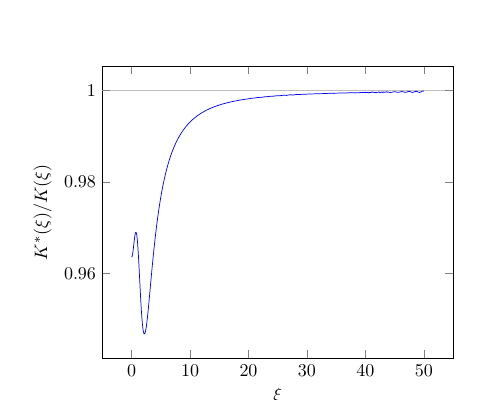
\begin{tikzpicture}[
scale=0.65,]\begin{axis}[
xlabel={$\xi$},
ylabel={$\fdfunc{K}^*(\xi)/\fdfunc{K}(\xi)$},
scaled x ticks = false,
x tick label style = {/pgf/number format/fixed},
scaled y ticks = false,
y tick label style = {/pgf/number format/fixed},
extra y ticks       = 1,
extra y tick labels = ,
extra y tick style  = { grid = major }
]
\addplot[color=blue,] coordinates {
(0.0000000000, 0.9635604621)
(0.0000500000, 0.9635604621)
(0.0002000000, 0.9635604630)
(0.0004500000, 0.9635604668)
(0.0008000000, 0.9635604771)
(0.0012500000, 0.9635604987)
(0.0018000000, 0.9635605379)
(0.0024500000, 0.9635606026)
(0.0032000000, 0.9635607018)
(0.0040500000, 0.9635608461)
(0.0050000000, 0.9635610473)
(0.0060500000, 0.9635613189)
(0.0072000000, 0.9635616756)
(0.0084500000, 0.9635621335)
(0.0098000000, 0.9635627101)
(0.0112500000, 0.9635634244)
(0.0128000000, 0.9635642967)
(0.0144500000, 0.9635653488)
(0.0162000000, 0.9635666036)
(0.0180500000, 0.9635680857)
(0.0200000000, 0.9635698210)
(0.0220500000, 0.9635718365)
(0.0242000000, 0.9635741609)
(0.0264500000, 0.9635768240)
(0.0288000000, 0.9635798571)
(0.0312500000, 0.9635832926)
(0.0338000000, 0.9635871645)
(0.0364500000, 0.9635915077)
(0.0392000000, 0.9635963585)
(0.0420500000, 0.9636017546)
(0.0450000000, 0.9636077348)
(0.0480500000, 0.9636143388)
(0.0512000000, 0.9636216078)
(0.0544500000, 0.9636295838)
(0.0578000000, 0.9636383102)
(0.0612500000, 0.9636478310)
(0.0648000000, 0.9636581914)
(0.0684500000, 0.9636694375)
(0.0722000000, 0.9636816162)
(0.0760500000, 0.9636947751)
(0.0800000000, 0.9637089625)
(0.0840500000, 0.9637242275)
(0.0882000000, 0.9637406197)
(0.0924500000, 0.9637581890)
(0.0968000000, 0.9637769859)
(0.1012500000, 0.9637970609)
(0.1058000000, 0.9638184651)
(0.1104500000, 0.9638412492)
(0.1152000000, 0.9638654641)
(0.1200500000, 0.9638911604)
(0.1250000000, 0.9639183885)
(0.1300500000, 0.9639471983)
(0.1352000000, 0.9639776390)
(0.1404500000, 0.9640097591)
(0.1458000000, 0.9640436063)
(0.1512500000, 0.9640792270)
(0.1568000000, 0.9641166665)
(0.1624500000, 0.9641559685)
(0.1682000000, 0.9641971752)
(0.1740500000, 0.9642403269)
(0.1800000000, 0.9642854616)
(0.1860500000, 0.9643326155)
(0.1922000000, 0.9643818218)
(0.1984500000, 0.9644331113)
(0.2048000000, 0.9644865118)
(0.2112500000, 0.9645420478)
(0.2178000000, 0.9645997402)
(0.2244500000, 0.9646596065)
(0.2312000000, 0.9647216599)
(0.2380500000, 0.9647859096)
(0.2450000000, 0.9648523601)
(0.2520500000, 0.9649210112)
(0.2592000000, 0.9649918576)
(0.2664500000, 0.9650648886)
(0.2738000000, 0.9651400878)
(0.2812500000, 0.9652174331)
(0.2888000000, 0.9652968959)
(0.2964500000, 0.9653784414)
(0.3042000000, 0.9654620277)
(0.3120500000, 0.9655476061)
(0.3200000000, 0.9656351204)
(0.3280500000, 0.9657245070)
(0.3362000000, 0.9658156942)
(0.3444500000, 0.9659086024)
(0.3528000000, 0.9660031435)
(0.3612500000, 0.9660992209)
(0.3698000000, 0.9661967292)
(0.3784500000, 0.9662955538)
(0.3872000000, 0.9663955711)
(0.3960500000, 0.9664966480)
(0.4050000000, 0.9665986420)
(0.4140500000, 0.9667014009)
(0.4232000000, 0.9668047625)
(0.4324500000, 0.9669085551)
(0.4418000000, 0.9670125969)
(0.4512500000, 0.9671166960)
(0.4608000000, 0.9672206507)
(0.4704500000, 0.9673242495)
(0.4802000000, 0.9674272709)
(0.4900500000, 0.9675294835)
(0.5000000000, 0.9676306465)
(0.5100500000, 0.9677305095)
(0.5202000000, 0.9678288129)
(0.5304500000, 0.9679252881)
(0.5408000000, 0.9680196579)
(0.5512500000, 0.9681116364)
(0.5618000000, 0.9682009302)
(0.5724500000, 0.9682872379)
(0.5832000000, 0.9683702514)
(0.5940500000, 0.9684496557)
(0.6050000000, 0.9685251300)
(0.6160500000, 0.9685963482)
(0.6272000000, 0.9686629792)
(0.6384500000, 0.9687246882)
(0.6498000000, 0.9687811371)
(0.6612500000, 0.9688319852)
(0.6728000000, 0.9688768903)
(0.6844500000, 0.9689155096)
(0.6962000000, 0.9689475005)
(0.7080500000, 0.9689725215)
(0.7200000000, 0.9689902334)
(0.7320500000, 0.9690003004)
(0.7442000000, 0.9690023909)
(0.7564500000, 0.9689961790)
(0.7688000000, 0.9689813453)
(0.7812500000, 0.9689575782)
(0.7938000000, 0.9689245751)
(0.8064500000, 0.9688820437)
(0.8192000000, 0.9688297032)
(0.8320500000, 0.9687672852)
(0.8450000000, 0.9686945354)
(0.8580500000, 0.9686112146)
(0.8712000000, 0.9685170999)
(0.8844500000, 0.9684119859)
(0.8978000000, 0.9682956860)
(0.9112500000, 0.9681680336)
(0.9248000000, 0.9680288829)
(0.9384500000, 0.9678781107)
(0.9522000000, 0.9677156163)
(0.9660500000, 0.9675413237)
(0.9800000000, 0.9673551820)
(0.9940500000, 0.9671571663)
(1.0082000000, 0.9669472785)
(1.0224500000, 0.9667255482)
(1.0368000000, 0.9664920333)
(1.0512500000, 0.9662468207)
(1.0658000000, 0.9659900264)
(1.0804500000, 0.9657217965)
(1.0952000000, 0.9654423071)
(1.1100500000, 0.9651517647)
(1.1250000000, 0.9648504060)
(1.1400500000, 0.9645384987)
(1.1552000000, 0.9642163402)
(1.1704500000, 0.9638842582)
(1.1858000000, 0.9635426103)
(1.2012500000, 0.9631917832)
(1.2168000000, 0.9628321923)
(1.2324500000, 0.9624642810)
(1.2482000000, 0.9620885199)
(1.2640500000, 0.9617054059)
(1.2800000000, 0.9613154609)
(1.2960500000, 0.9609192312)
(1.3122000000, 0.9605172854)
(1.3284500000, 0.9601102140)
(1.3448000000, 0.9596986269)
(1.3612500000, 0.9592831528)
(1.3778000000, 0.9588644369)
(1.3944500000, 0.9584431395)
(1.4112000000, 0.9580199340)
(1.4280500000, 0.9575955053)
(1.4450000000, 0.9571705475)
(1.4620500000, 0.9567457621)
(1.4792000000, 0.9563218561)
(1.4964500000, 0.9558995396)
(1.5138000000, 0.9554795242)
(1.5312500000, 0.9550625206)
(1.5488000000, 0.9546492364)
(1.5664500000, 0.9542403743)
(1.5842000000, 0.9538366300)
(1.6020500000, 0.9534386898)
(1.6200000000, 0.9530472291)
(1.6380500000, 0.9526629100)
(1.6562000000, 0.9522863797)
(1.6744500000, 0.9519182685)
(1.6928000000, 0.9515591880)
(1.7112500000, 0.9512097297)
(1.7298000000, 0.9508704628)
(1.7484500000, 0.9505419333)
(1.7672000000, 0.9502246624)
(1.7860500000, 0.9499191451)
(1.8050000000, 0.9496258490)
(1.8240500000, 0.9493452135)
(1.8432000000, 0.9490776485)
(1.8624500000, 0.9488235338)
(1.8818000000, 0.9485832185)
(1.9012500000, 0.9483570202)
(1.9208000000, 0.9481452246)
(1.9404500000, 0.9479480854)
(1.9602000000, 0.9477658240)
(1.9800500000, 0.9475986293)
(2.0000000000, 0.9474466581)
(2.0200500000, 0.9473100350)
(2.0402000000, 0.9471888530)
(2.0604500000, 0.9470831735)
(2.0808000000, 0.9469930273)
(2.1012500000, 0.9469184150)
(2.1218000000, 0.9468593077)
(2.1424500000, 0.9468156481)
(2.1632000000, 0.9467873509)
(2.1840500000, 0.9467743046)
(2.2050000000, 0.9467763715)
(2.2260500000, 0.9467933898)
(2.2472000000, 0.9468251742)
(2.2684500000, 0.9468715174)
(2.2898000000, 0.9469321911)
(2.3112500000, 0.9470069476)
(2.3328000000, 0.9470955209)
(2.3544500000, 0.9471976281)
(2.3762000000, 0.9473129708)
(2.3980500000, 0.9474412364)
(2.4200000000, 0.9475820995)
(2.4420500000, 0.9477352231)
(2.4642000000, 0.9479002600)
(2.4864500000, 0.9480768542)
(2.5088000000, 0.9482646420)
(2.5312500000, 0.9484632535)
(2.5538000000, 0.9486723132)
(2.5764500000, 0.9488914421)
(2.5992000000, 0.9491202581)
(2.6220500000, 0.9493583770)
(2.6450000000, 0.9496054142)
(2.6680500000, 0.9498609852)
(2.6912000000, 0.9501247065)
(2.7144500000, 0.9503961965)
(2.7378000000, 0.9506750765)
(2.7612500000, 0.9509609715)
(2.7848000000, 0.9512535103)
(2.8084500000, 0.9515523270)
(2.8322000000, 0.9518570609)
(2.8560500000, 0.9521673575)
(2.8800000000, 0.9524828688)
(2.9040500000, 0.9528032535)
(2.9282000000, 0.9531281779)
(2.9524500000, 0.9534573158)
(2.9768000000, 0.9537903489)
(3.0012500000, 0.9541269674)
(3.0258000000, 0.9544668694)
(3.0504500000, 0.9548097750)
(3.0752000000, 0.9551553608)
(3.1000500000, 0.9555033902)
(3.1250000000, 0.9558535834)
(3.1500500000, 0.9562056826)
(3.1752000000, 0.9565594387)
(3.2004500000, 0.9569146116)
(3.2258000000, 0.9572709699)
(3.2512500000, 0.9576282910)
(3.2768000000, 0.9579863607)
(3.3024500000, 0.9583449737)
(3.3282000000, 0.9587039328)
(3.3540500000, 0.9590630491)
(3.3800000000, 0.9594221420)
(3.4060500000, 0.9597810387)
(3.4322000000, 0.9601395742)
(3.4584500000, 0.9604975910)
(3.4848000000, 0.9608549392)
(3.5112500000, 0.9612114760)
(3.5378000000, 0.9615670657)
(3.5644500000, 0.9619215794)
(3.5912000000, 0.9622748949)
(3.6180500000, 0.9626268963)
(3.6450000000, 0.9629774741)
(3.6720500000, 0.9633265247)
(3.6992000000, 0.9636739506)
(3.7264500000, 0.9640196596)
(3.7538000000, 0.9643635651)
(3.7812500000, 0.9647055859)
(3.8088000000, 0.9650456457)
(3.8364500000, 0.9653836731)
(3.8642000000, 0.9657196014)
(3.8920500000, 0.9660533686)
(3.9200000000, 0.9663849168)
(3.9480500000, 0.9667141923)
(3.9762000000, 0.9670411457)
(4.0044500000, 0.9673657311)
(4.0328000000, 0.9676879064)
(4.0612500000, 0.9680076331)
(4.0898000000, 0.9683248760)
(4.1184500000, 0.9686396032)
(4.1472000000, 0.9689517859)
(4.1760500000, 0.9692613982)
(4.2050000000, 0.9695684170)
(4.2340500000, 0.9698728221)
(4.2632000000, 0.9701745955)
(4.2924500000, 0.9704737221)
(4.3218000000, 0.9707701888)
(4.3512500000, 0.9710639848)
(4.3808000000, 0.9713551016)
(4.4104500000, 0.9716435324)
(4.4402000000, 0.9719292726)
(4.4700500000, 0.9722123192)
(4.5000000000, 0.9724926712)
(4.5300500000, 0.9727703288)
(4.5602000000, 0.9730452942)
(4.5904500000, 0.9733175707)
(4.6208000000, 0.9735871632)
(4.6512500000, 0.9738540779)
(4.6818000000, 0.9741183221)
(4.7124500000, 0.9743799043)
(4.7432000000, 0.9746388342)
(4.7740500000, 0.9748951224)
(4.8050000000, 0.9751487805)
(4.8360500000, 0.9753998210)
(4.8672000000, 0.9756482573)
(4.8984500000, 0.9758941036)
(4.9298000000, 0.9761373747)
(4.9612500000, 0.9763780861)
(4.9928000000, 0.9766162543)
(5.0244500000, 0.9768518958)
(5.0562000000, 0.9770850281)
(5.0880500000, 0.9773156691)
(5.1200000000, 0.9775438371)
(5.1520500000, 0.9777695508)
(5.1842000000, 0.9779928294)
(5.2164500000, 0.9782136924)
(5.2488000000, 0.9784321597)
(5.2812500000, 0.9786482513)
(5.3138000000, 0.9788619877)
(5.3464500000, 0.9790733895)
(5.3792000000, 0.9792824776)
(5.4120500000, 0.9794892729)
(5.4450000000, 0.9796937966)
(5.4780500000, 0.9798960701)
(5.5112000000, 0.9800961147)
(5.5444500000, 0.9802939520)
(5.5778000000, 0.9804896036)
(5.6112500000, 0.9806830910)
(5.6448000000, 0.9808744360)
(5.6784500000, 0.9810636603)
(5.7122000000, 0.9812507856)
(5.7460500000, 0.9814358336)
(5.7800000000, 0.9816188258)
(5.8140500000, 0.9817997840)
(5.8482000000, 0.9819787298)
(5.8824500000, 0.9821556846)
(5.9168000000, 0.9823306699)
(5.9512500000, 0.9825037071)
(5.9858000000, 0.9826748174)
(6.0204500000, 0.9828440220)
(6.0552000000, 0.9830113419)
(6.0900500000, 0.9831767982)
(6.1250000000, 0.9833404117)
(6.1600500000, 0.9835022029)
(6.1952000000, 0.9836621926)
(6.2304500000, 0.9838204011)
(6.2658000000, 0.9839768487)
(6.3012500000, 0.9841315555)
(6.3368000000, 0.9842845414)
(6.3724500000, 0.9844358264)
(6.4082000000, 0.9845854300)
(6.4440500000, 0.9847333717)
(6.4800000000, 0.9848796708)
(6.5160500000, 0.9850243465)
(6.5522000000, 0.9851674177)
(6.5884500000, 0.9853089032)
(6.6248000000, 0.9854488216)
(6.6612500000, 0.9855871914)
(6.6978000000, 0.9857240308)
(6.7344500000, 0.9858593578)
(6.7712000000, 0.9859931903)
(6.8080500000, 0.9861255462)
(6.8450000000, 0.9862564427)
(6.8820500000, 0.9863858974)
(6.9192000000, 0.9865139273)
(6.9564500000, 0.9866405494)
(6.9938000000, 0.9867657805)
(7.0312500000, 0.9868896372)
(7.0688000000, 0.9870121358)
(7.1064500000, 0.9871332927)
(7.1442000000, 0.9872531238)
(7.1820500000, 0.9873716450)
(7.2200000000, 0.9874888720)
(7.2580500000, 0.9876048202)
(7.2962000000, 0.9877195051)
(7.3344500000, 0.9878329417)
(7.3728000000, 0.9879451451)
(7.4112500000, 0.9880561299)
(7.4498000000, 0.9881659108)
(7.4884500000, 0.9882745022)
(7.5272000000, 0.9883819184)
(7.5660500000, 0.9884881735)
(7.6050000000, 0.9885932814)
(7.6440500000, 0.9886972559)
(7.6832000000, 0.9888001104)
(7.7224500000, 0.9889018585)
(7.7618000000, 0.9890025135)
(7.8012500000, 0.9891020883)
(7.8408000000, 0.9892005959)
(7.8804500000, 0.9892980491)
(7.9202000000, 0.9893944606)
(7.9600500000, 0.9894898426)
(8.0000000000, 0.9895842077)
(8.0400500000, 0.9896775678)
(8.0802000000, 0.9897699350)
(8.1204500000, 0.9898613212)
(8.1608000000, 0.9899517380)
(8.2012500000, 0.9900411970)
(8.2418000000, 0.9901297095)
(8.2824500000, 0.9902172869)
(8.3232000000, 0.9903039403)
(8.3640500000, 0.9903896806)
(8.4050000000, 0.9904745188)
(8.4460500000, 0.9905584654)
(8.4872000000, 0.9906415310)
(8.5284500000, 0.9907237262)
(8.5698000000, 0.9908050611)
(8.6112500000, 0.9908855460)
(8.6528000000, 0.9909651909)
(8.6944500000, 0.9910440057)
(8.7362000000, 0.9911220003)
(8.7780500000, 0.9911991842)
(8.8200000000, 0.9912755670)
(8.8620500000, 0.9913511582)
(8.9042000000, 0.9914259670)
(8.9464500000, 0.9915000027)
(8.9888000000, 0.9915732742)
(9.0312500000, 0.9916457906)
(9.0738000000, 0.9917175607)
(9.1164500000, 0.9917885932)
(9.1592000000, 0.9918588967)
(9.2020500000, 0.9919284797)
(9.2450000000, 0.9919973507)
(9.2880500000, 0.9920655179)
(9.3312000000, 0.9921329895)
(9.3744500000, 0.9921997736)
(9.4178000000, 0.9922658782)
(9.4612500000, 0.9923313111)
(9.5048000000, 0.9923960802)
(9.5484500000, 0.9924601931)
(9.5922000000, 0.9925236574)
(9.6360500000, 0.9925864805)
(9.6800000000, 0.9926486700)
(9.7240500000, 0.9927102330)
(9.7682000000, 0.9927711768)
(9.8124500000, 0.9928315086)
(9.8568000000, 0.9928912352)
(9.9012500000, 0.9929503638)
(9.9458000000, 0.9930089010)
(9.9904500000, 0.9930668538)
(10.0352000000, 0.9931242287)
(10.0800500000, 0.9931810324)
(10.1250000000, 0.9932372713)
(10.1700500000, 0.9932929520)
(10.2152000000, 0.9933480807)
(10.2604500000, 0.9934026637)
(10.3058000000, 0.9934567073)
(10.3512500000, 0.9935102175)
(10.3968000000, 0.9935632004)
(10.4424500000, 0.9936156619)
(10.4882000000, 0.9936676080)
(10.5340500000, 0.9937190444)
(10.5800000000, 0.9937699769)
(10.6260500000, 0.9938204111)
(10.6722000000, 0.9938703527)
(10.7184500000, 0.9939198072)
(10.7648000000, 0.9939687800)
(10.8112500000, 0.9940172766)
(10.8578000000, 0.9940653023)
(10.9044500000, 0.9941128623)
(10.9512000000, 0.9941599618)
(10.9980500000, 0.9942066059)
(11.0450000000, 0.9942527999)
(11.0920500000, 0.9942985485)
(11.1392000000, 0.9943438568)
(11.1864500000, 0.9943887297)
(11.2338000000, 0.9944331720)
(11.2812500000, 0.9944771884)
(11.3288000000, 0.9945207837)
(11.3764500000, 0.9945639624)
(11.4242000000, 0.9946067293)
(11.4720500000, 0.9946490888)
(11.5200000000, 0.9946910454)
(11.5680500000, 0.9947326035)
(11.6162000000, 0.9947737676)
(11.6644500000, 0.9948145418)
(11.7128000000, 0.9948549305)
(11.7612500000, 0.9948949379)
(11.8098000000, 0.9949345682)
(11.8584500000, 0.9949738254)
(11.9072000000, 0.9950127136)
(11.9560500000, 0.9950512369)
(12.0050000000, 0.9950893992)
(12.0540500000, 0.9951272043)
(12.1032000000, 0.9951646563)
(12.1524500000, 0.9952017588)
(12.2018000000, 0.9952385158)
(12.2512500000, 0.9952749334)
(12.3008000000, 0.9953110075)
(12.3504500000, 0.9953467497)
(12.4002000000, 0.9953821609)
(12.4500500000, 0.9954172446)
(12.5000000000, 0.9954520045)
(12.5500500000, 0.9954864438)
(12.6002000000, 0.9955205662)
(12.6504500000, 0.9955543748)
(12.7008000000, 0.9955878732)
(12.7512500000, 0.9956210646)
(12.8018000000, 0.9956539426)
(12.8524500000, 0.9956865225)
(12.9032000000, 0.9957188292)
(12.9540500000, 0.9957508248)
(13.0050000000, 0.9957825294)
(13.0560500000, 0.9958139460)
(13.1072000000, 0.9958450776)
(13.1584500000, 0.9958759273)
(13.2098000000, 0.9959064980)
(13.2612500000, 0.9959367927)
(13.3128000000, 0.9959668142)
(13.3644500000, 0.9959966032)
(13.4162000000, 0.9960261028)
(13.4680500000, 0.9960553342)
(13.5200000000, 0.9960842257)
(13.5720500000, 0.9961129237)
(13.6242000000, 0.9961413653)
(13.6764500000, 0.9961695532)
(13.7288000000, 0.9961974898)
(13.7812500000, 0.9962251779)
(13.8338000000, 0.9962526201)
(13.8864500000, 0.9962798188)
(13.9392000000, 0.9963067765)
(13.9920500000, 0.9963333515)
(14.0450000000, 0.9963599793)
(14.0980500000, 0.9963862291)
(14.1512000000, 0.9964122478)
(14.2044500000, 0.9964380377)
(14.2578000000, 0.9964636012)
(14.3112500000, 0.9964889406)
(14.3648000000, 0.9965140582)
(14.4184500000, 0.9965389562)
(14.4722000000, 0.9965636369)
(14.5260500000, 0.9965881025)
(14.5800000000, 0.9966123552)
(14.6340500000, 0.9966363972)
(14.6882000000, 0.9966602305)
(14.7424500000, 0.9966838574)
(14.7968000000, 0.9967072798)
(14.8512500000, 0.9967304999)
(14.9058000000, 0.9967535197)
(14.9604500000, 0.9967763413)
(15.0152000000, 0.9967989665)
(15.0700500000, 0.9968213974)
(15.1250000000, 0.9968436360)
(15.1800500000, 0.9968656842)
(15.2352000000, 0.9968875438)
(15.2904500000, 0.9969092168)
(15.3458000000, 0.9969307050)
(15.4012500000, 0.9969520102)
(15.4568000000, 0.9969731344)
(15.5124500000, 0.9969940792)
(15.5682000000, 0.9970148465)
(15.6240500000, 0.9970354381)
(15.6800000000, 0.9970558556)
(15.7360500000, 0.9970761008)
(15.7922000000, 0.9970961754)
(15.8484500000, 0.9971160811)
(15.9048000000, 0.9971358195)
(15.9612500000, 0.9971553923)
(16.0178000000, 0.9971748012)
(16.0744500000, 0.9971940477)
(16.1312000000, 0.9972131333)
(16.1880500000, 0.9972320598)
(16.2450000000, 0.9972508287)
(16.3020500000, 0.9972694414)
(16.3592000000, 0.9972878995)
(16.4164500000, 0.9973062046)
(16.4738000000, 0.9973243580)
(16.5312500000, 0.9973423613)
(16.5888000000, 0.9973602160)
(16.6464500000, 0.9973779235)
(16.7042000000, 0.9973954851)
(16.7620500000, 0.9974129023)
(16.8200000000, 0.9974301766)
(16.8780500000, 0.9974473092)
(16.9362000000, 0.9974643016)
(16.9944500000, 0.9974811550)
(17.0528000000, 0.9974978709)
(17.1112500000, 0.9975144505)
(17.1698000000, 0.9975308951)
(17.2284500000, 0.9975472061)
(17.2872000000, 0.9975633847)
(17.3460500000, 0.9975794322)
(17.4050000000, 0.9975953498)
(17.4640500000, 0.9976161258)
(17.5232000000, 0.9976268003)
(17.5824500000, 0.9976423356)
(17.6418000000, 0.9976577459)
(17.7012500000, 0.9976730323)
(17.7608000000, 0.9976881961)
(17.8204500000, 0.9977032384)
(17.8802000000, 0.9977181603)
(17.9400500000, 0.9977264801)
(18.0000000000, 0.9977405475)
(18.0600500000, 0.9977554775)
(18.1202000000, 0.9977766669)
(18.1804500000, 0.9977910037)
(18.2408000000, 0.9978052268)
(18.3012500000, 0.9978193372)
(18.3618000000, 0.9978333360)
(18.4224500000, 0.9978472242)
(18.4832000000, 0.9978610028)
(18.5440500000, 0.9978746729)
(18.6050000000, 0.9978882354)
(18.6660500000, 0.9979070390)
(18.7272000000, 0.9979168728)
(18.7884500000, 0.9979282876)
(18.8498000000, 0.9979414298)
(18.9112500000, 0.9979544694)
(18.9728000000, 0.9979674072)
(19.0344500000, 0.9979802440)
(19.0962000000, 0.9979820774)
(19.1580500000, 0.9979975383)
(19.2200000000, 0.9980142409)
(19.2820500000, 0.9980316513)
(19.3442000000, 0.9980429496)
(19.4064500000, 0.9980552010)
(19.4688000000, 0.9980673579)
(19.5312500000, 0.9980794212)
(19.5938000000, 0.9980913916)
(19.6564500000, 0.9981145582)
(19.7192000000, 0.9981215856)
(19.7820500000, 0.9981273274)
(19.8450000000, 0.9981326018)
(19.9080500000, 0.9981383244)
(19.9712000000, 0.9981453774)
(20.0344500000, 0.9981726558)
(20.0978000000, 0.9981839128)
(20.1612500000, 0.9981950855)
(20.2248000000, 0.9982061717)
(20.2884500000, 0.9982171761)
(20.3522000000, 0.9982330761)
(20.4160500000, 0.9982511556)
(20.4800000000, 0.9982676634)
(20.5440500000, 0.9982816825)
(20.6082000000, 0.9982709586)
(20.6724500000, 0.9982814747)
(20.7368000000, 0.9982919110)
(20.8012500000, 0.9983022688)
(20.8658000000, 0.9983087026)
(20.9304500000, 0.9983101305)
(20.9952000000, 0.9983130118)
(21.0600500000, 0.9983184869)
(21.1250000000, 0.9983273430)
(21.1900500000, 0.9983398818)
(21.2552000000, 0.9983726357)
(21.3204500000, 0.9983823917)
(21.3858000000, 0.9983920759)
(21.4512500000, 0.9984016890)
(21.5168000000, 0.9984328727)
(21.5824500000, 0.9984482431)
(21.6482000000, 0.9984596315)
(21.7140500000, 0.9984394379)
(21.7800000000, 0.9984693610)
(21.8460500000, 0.9984579016)
(21.9122000000, 0.9984670300)
(21.9784500000, 0.9984760910)
(22.0448000000, 0.9984850853)
(22.1112500000, 0.9984633808)
(22.1778000000, 0.9984693654)
(22.2444500000, 0.9984802438)
(22.3112000000, 0.9984958599)
(22.3780500000, 0.9985153241)
(22.4450000000, 0.9985376994)
(22.5120500000, 0.9985462440)
(22.5792000000, 0.9985547323)
(22.6464500000, 0.9985631597)
(22.7138000000, 0.9985715231)
(22.7812500000, 0.9986154904)
(22.8488000000, 0.9986164117)
(22.9164500000, 0.9986127641)
(22.9842000000, 0.9986062254)
(23.0520500000, 0.9986124551)
(23.1200000000, 0.9986204630)
(23.1880500000, 0.9986284135)
(23.2562000000, 0.9986363134)
(23.3244500000, 0.9986441541)
(23.3928000000, 0.9986200692)
(23.4612500000, 0.9986407902)
(23.5298000000, 0.9986646746)
(23.5984500000, 0.9986893089)
(23.6672000000, 0.9986825343)
(23.7360500000, 0.9986900507)
(23.8050000000, 0.9986975127)
(23.8740500000, 0.9987049110)
(23.9432000000, 0.9987122663)
(24.0124500000, 0.9987402396)
(24.0818000000, 0.9987296477)
(24.1512500000, 0.9987181711)
(24.2208000000, 0.9987086978)
(24.2904500000, 0.9987482622)
(24.3602000000, 0.9987553149)
(24.4300500000, 0.9987623305)
(24.5000000000, 0.9987692842)
(24.5700500000, 0.9987545408)
(24.6402000000, 0.9987809798)
(24.7104500000, 0.9988080913)
(24.7808000000, 0.9988327003)
(24.8512500000, 0.9988033579)
(24.9218000000, 0.9988100181)
(24.9924500000, 0.9988166272)
(25.0632000000, 0.9988232057)
(25.1340500000, 0.9988512964)
(25.2050000000, 0.9988363686)
(25.2760500000, 0.9988209781)
(25.3472000000, 0.9988085840)
(25.4184500000, 0.9988022349)
(25.4898000000, 0.9988617345)
(25.5612500000, 0.9988680347)
(25.6328000000, 0.9988742286)
(25.7044500000, 0.9988804119)
(25.7762000000, 0.9988897476)
(25.8480500000, 0.9989190385)
(25.9200000000, 0.9989444450)
(25.9920500000, 0.9989627877)
(26.0642000000, 0.9989106544)
(26.1364500000, 0.9989165329)
(26.2088000000, 0.9989223840)
(26.2812500000, 0.9989283921)
(26.3538000000, 0.9989260400)
(26.4264500000, 0.9989075668)
(26.4992000000, 0.9988939415)
(26.5720500000, 0.9988883942)
(26.6450000000, 0.9989572605)
(26.7180500000, 0.9989629674)
(26.7912000000, 0.9989685960)
(26.8644500000, 0.9989738473)
(26.9378000000, 0.9989943075)
(27.0112500000, 0.9990246212)
(27.0848000000, 0.9990487175)
(27.1584500000, 0.9990634326)
(27.2322000000, 0.9990006285)
(27.3060500000, 0.9990058806)
(27.3800000000, 0.9990111905)
(27.4540500000, 0.9990216125)
(27.5282000000, 0.9989985636)
(27.6024500000, 0.9989790283)
(27.6768000000, 0.9989671679)
(27.7512500000, 0.9989659256)
(27.8258000000, 0.9990435216)
(27.9004500000, 0.9990485654)
(27.9752000000, 0.9990534066)
(28.0500500000, 0.9990627934)
(28.1250000000, 0.9990967652)
(28.2000500000, 0.9991253375)
(28.2752000000, 0.9990715477)
(28.3504500000, 0.9990761906)
(28.4258000000, 0.9990810416)
(28.5012500000, 0.9990861288)
(28.5768000000, 0.9990918346)
(28.6524500000, 0.9990795118)
(28.7282000000, 0.9990554414)
(28.8040500000, 0.9991059539)
(28.8800000000, 0.9991125029)
(28.9560500000, 0.9991170646)
(29.0322000000, 0.9991211860)
(29.1084500000, 0.9991243586)
(29.1848000000, 0.9991288860)
(29.2612500000, 0.9991333843)
(29.3378000000, 0.9991378537)
(29.4144500000, 0.9991422944)
(29.4912000000, 0.9991467068)
(29.5680500000, 0.9991510911)
(29.6450000000, 0.9991554476)
(29.7220500000, 0.9991597764)
(29.7992000000, 0.9991640777)
(29.8764500000, 0.9991683516)
(29.9538000000, 0.9991725982)
(30.0312500000, 0.9991768179)
(30.1088000000, 0.9991810107)
(30.1864500000, 0.9991851770)
(30.2642000000, 0.9991893170)
(30.3420500000, 0.9991934311)
(30.4200000000, 0.9991975195)
(30.4980500000, 0.9992015822)
(30.5762000000, 0.9992056194)
(30.6544500000, 0.9992096312)
(30.7328000000, 0.9992136175)
(30.8112500000, 0.9992175787)
(30.8898000000, 0.9992215151)
(30.9684500000, 0.9992254268)
(31.0472000000, 0.9992293144)
(31.1260500000, 0.9992331779)
(31.2050000000, 0.9992370177)
(31.2840500000, 0.9992408337)
(31.3632000000, 0.9992446260)
(31.4424500000, 0.9992483944)
(31.5218000000, 0.9992521391)
(31.6012500000, 0.9992558604)
(31.6808000000, 0.9992595586)
(31.7604500000, 0.9992632342)
(31.8402000000, 0.9992668875)
(31.9200500000, 0.9992795468)
(32.0000000000, 0.9992868724)
(32.0800500000, 0.9992843133)
(32.1602000000, 0.9992812795)
(32.2404500000, 0.9992848218)
(32.3208000000, 0.9992883419)
(32.4012500000, 0.9992842029)
(32.4818000000, 0.9992814509)
(32.5624500000, 0.9992814587)
(32.6432000000, 0.9992838183)
(32.7240500000, 0.9993056253)
(32.8050000000, 0.9993090202)
(32.8860500000, 0.9993123942)
(32.9672000000, 0.9993157471)
(33.0484500000, 0.9993190789)
(33.1298000000, 0.9993223901)
(33.2112500000, 0.9993546237)
(33.2928000000, 0.9993177485)
(33.3744500000, 0.9993322062)
(33.4562000000, 0.9993354404)
(33.5380500000, 0.9993386555)
(33.6200000000, 0.9993418510)
(33.7020500000, 0.9993450265)
(33.7842000000, 0.9993291524)
(33.8664500000, 0.9993545754)
(33.9488000000, 0.9993544346)
(34.0312500000, 0.9993575335)
(34.1138000000, 0.9993606150)
(34.1964500000, 0.9993636793)
(34.2792000000, 0.9993667259)
(34.3620500000, 0.9993697542)
(34.4450000000, 0.9993747849)
(34.5280500000, 0.9993348342)
(34.6112000000, 0.9993787248)
(34.6944500000, 0.9993816781)
(34.7778000000, 0.9993846147)
(34.8612500000, 0.9993875354)
(34.9448000000, 0.9993904403)
(35.0284500000, 0.9993891008)
(35.1122000000, 0.9993962004)
(35.1960500000, 0.9993990538)
(35.2800000000, 0.9994018887)
(35.3640500000, 0.9994047055)
(35.4482000000, 0.9994075054)
(35.5324500000, 0.9994102897)
(35.6168000000, 0.9994130597)
(35.7012500000, 0.9994158149)
(35.7858000000, 0.9994185554)
(35.8704500000, 0.9994212797)
(35.9552000000, 0.9993977791)
(36.0400500000, 0.9994226380)
(36.1250000000, 0.9994293473)
(36.2100500000, 0.9994320034)
(36.2952000000, 0.9994346447)
(36.3804500000, 0.9994372729)
(36.4658000000, 0.9994398881)
(36.5512500000, 0.9994424895)
(36.6368000000, 0.9994330546)
(36.7224500000, 0.9994476454)
(36.8082000000, 0.9994531670)
(36.8940500000, 0.9994146075)
(36.9800000000, 0.9994552528)
(37.0660500000, 0.9994577600)
(37.1522000000, 0.9994602553)
(37.2384500000, 0.9994627388)
(37.3248000000, 0.9994652090)
(37.4112500000, 0.9994635447)
(37.4978000000, 0.9994701056)
(37.5844500000, 0.9995064591)
(37.6712000000, 0.9994749358)
(37.7580500000, 0.9994773288)
(37.8450000000, 0.9994797100)
(37.9320500000, 0.9994820806)
(38.0192000000, 0.9994844405)
(38.1064500000, 0.9994497512)
(38.1938000000, 0.9994169735)
(38.2812500000, 0.9995022278)
(38.3688000000, 0.9994937404)
(38.4564500000, 0.9994960280)
(38.5442000000, 0.9994983006)
(38.6320500000, 0.9994986908)
(38.7200000000, 0.9995028178)
(38.8080500000, 0.9995050617)
(38.8962000000, 0.9995072940)
(38.9844500000, 0.9994563796)
(39.0728000000, 0.9995117167)
(39.1612500000, 0.9995139030)
(39.2498000000, 0.9995079084)
(39.3384500000, 0.9995063776)
(39.4272000000, 0.9995406864)
(39.5160500000, 0.9995705353)
(39.6050000000, 0.9995246639)
(39.6940500000, 0.9995267895)
(39.7832000000, 0.9995288988)
(39.8724500000, 0.9995577213)
(39.9618000000, 0.9996094611)
(40.0512500000, 0.9994935598)
(40.1408000000, 0.9995371929)
(40.2304500000, 0.9995392428)
(40.3202000000, 0.9995412820)
(40.4100500000, 0.9995484996)
(40.5000000000, 0.9994935732)
(40.5900500000, 0.9994499507)
(40.6802000000, 0.9995493314)
(40.7704500000, 0.9995513080)
(40.8608000000, 0.9995532711)
(40.9512500000, 0.9995552296)
(41.0418000000, 0.9995813062)
(41.1324500000, 0.9996367610)
(41.2232000000, 0.9996741084)
(41.3140500000, 0.9995629817)
(41.4050000000, 0.9995648904)
(41.4960500000, 0.9995134643)
(41.5872000000, 0.9995717666)
(41.6784500000, 0.9995885310)
(41.7698000000, 0.9994752556)
(41.8612500000, 0.9994567764)
(41.9528000000, 0.9995761101)
(42.0444500000, 0.9995779526)
(42.1362000000, 0.9995525307)
(42.2280500000, 0.9996097588)
(42.3200000000, 0.9996591804)
(42.4120500000, 0.9995851907)
(42.5042000000, 0.9995072212)
(42.5964500000, 0.9995887522)
(42.6888000000, 0.9996370896)
(42.7812500000, 0.9995886605)
(42.8738000000, 0.9996342043)
(42.9664500000, 0.9995101518)
(43.0592000000, 0.9995975158)
(43.1520500000, 0.9996723021)
(43.2450000000, 0.9996009380)
(43.3380500000, 0.9995842426)
(43.4312000000, 0.9996301418)
(43.5244500000, 0.9996683845)
(43.6178000000, 0.9996911763)
(43.7112500000, 0.9996093812)
(43.8048000000, 0.9996110390)
(43.8984500000, 0.9996497154)
(43.9922000000, 0.9996135723)
(44.0860500000, 0.9995792414)
(44.1800000000, 0.9995542887)
(44.2740500000, 0.9995438547)
(44.3682000000, 0.9995497597)
(44.4624500000, 0.9995703674)
(44.5568000000, 0.9996011533)
(44.6512500000, 0.9996357873)
(44.7458000000, 0.9996674688)
(44.8404500000, 0.9996902406)
(44.9352000000, 0.9997000587)
(45.0300500000, 0.9996954617)
(45.1250000000, 0.9996777704)
(45.2200500000, 0.9996508148)
(45.3152000000, 0.9996202440)
(45.4104500000, 0.9995925201)
(45.5058000000, 0.9995737347)
(45.6012500000, 0.9995684229)
(45.6968000000, 0.9995785751)
(45.7924500000, 0.9996030528)
(45.8882000000, 0.9996375758)
(45.9840500000, 0.9996753704)
(46.0800000000, 0.9997084368)
(46.1760500000, 0.9997292424)
(46.2722000000, 0.9997325068)
(46.3684500000, 0.9997166619)
(46.4648000000, 0.9996845799)
(46.5612500000, 0.9996432898)
(46.6578000000, 0.9996026215)
(46.7544500000, 0.9995729986)
(46.8512000000, 0.9995628536)
(46.9480500000, 0.9995763063)
(47.0450000000, 0.9996117496)
(47.1420500000, 0.9996618134)
(47.2392000000, 0.9997148509)
(47.3364500000, 0.9997576874)
(47.4338000000, 0.9997789964)
(47.5312500000, 0.9997724350)
(47.6288000000, 0.9997386623)
(47.7264500000, 0.9996855992)
(47.8242000000, 0.9996267311)
(47.9220500000, 0.9995777839)
(48.0200000000, 0.9995525865)
(48.1180500000, 0.9995592156)
(48.2162000000, 0.9995975100)
(48.3144500000, 0.9996587251)
(48.4128000000, 0.9997275375)
(48.5112500000, 0.9997859628)
(48.6098000000, 0.9996932271)
(48.7084500000, 0.9998149842)
(48.8072000000, 0.9997765273)
(48.9060500000, 0.9997126413)
(49.0050000000, 0.9996404271)
(49.1040500000, 0.9995797632)
(49.2032000000, 0.9995478901)
(49.3024500000, 0.9995545595)
(49.4018000000, 0.9995991238)
(49.5012500000, 0.9996704407)
(49.6008000000, 0.9997497052)
(49.7004500000, 0.9998154970)
(49.8002000000, 0.9998496919)
(49.9000500000, 0.9998425997)
(50.0000000000, 0.9997958614)
};
\end{axis}\end{tikzpicture}
}
    \caption{Comparison of the \idxs{impulse}{response} of \eqref{eq:empirical} and the impulse response of an ideal kernel. The fluctuations for the higher values of $\xi$ in \subrefp{fig:transformedkernelratio} are purely due to \idxs{numerical}{errors}.}
    \label{fig:transformedkernel}
\end{figure}

Expanding \eqref{eq:opcfconvolution} yields

\begin{equation} \label{eq:opcfintegral}
\sop{C}\,\eta(\vec{r},\,t) = \iint f(\Delta\vec{r})\,\eta(\vec{r}-\Delta\vec{r},\,t)\,\opd\Delta\vec{r}
\end{equation}

which, by using \eqref{eq:ftokernel}, can be rewritten to

\begin{equation} \label{eq:opchunknown}
\sop{C}_h\,\eta(\vec{r},\,t) = a_h\iint K\left(\frac{\Delta\vec{r}}{h}\right)\,\eta(\vec{r}-\Delta\vec{r},\,t)\,\opd\Delta\vec{r},
\end{equation}

where the index $h$ is introduced to make it apparent that $\sop{C}$ is actually a function of the \idxs{water}{depth} $h$, and where

\begin{equation} \label{eq:aofh}
a_h = 1/h^2.
\end{equation}

We could just use this definition of $\sop{C}$ and plug it into \eqref{eq:diffeqspatial} and, by being \naive and \assuming that since \eqref{eq:diffeqspatial} is independent of $\vec{k}$, it would describe not only the behavior of single wave components fixed to a specific wave vector $\vec{k}$ which are described by \eqref{eq:component}, but the behavior of any free surface elevation $\eta(\vec{r},\,t)$, we would have a \PDE that we could use for simulating single wave components as well as complex (in the sense of being non-simple) surfaces.

A problem, though, is that $h$ is not a constant unless the sea bottom is perfectly flat, but dependent on the location, so \eqref{eq:opchunknown} is not directly applicable. The simplest remedy for this would be to just substitute $h$ for the water depth of the local position $h(\vec{r})$:

\begin{equation} \label{eq:opchlocal}
\sop{C}_{h(\vec{r})}\,\eta(\vec{r},\,t) = a_{h(\vec{r})}\iint K\left(\frac{\Delta\vec{r}}{h(\vec{r})}\right)\,\eta(\vec{r}-\Delta\vec{r},\,t)\,\opd\Delta\vec{r},
\end{equation}

where $a_{h(\vec{r})} = 1/h^2(\vec{r})$. Unfortunately, this method has other problems that occur when the bottom topography is unpleasant. For example, if one part of the water is surrounded by ground, as is the case with lakes, this simple version of the operator would be affected by parts of the water from which $\vec{r}$ is isolated. Hence, waves in one lake could, similar to in \idxs{quantum}{mechanics}, \tunnel into another, nearby lake, which is not the case in reality.

A possible remedy for this problem is to try to limit the convolution filter and let the kernel approach zero more quickly when the water gets shallower. For example, one could be to find the path from $\vec{r}$ to $\vec{r}-\Delta\vec{r}$ with the maximal minimal water depth, and use the minimal water depth of that path as an \idxs{effective}{water depth} $h_e$ for that sampling location. Another possibility could be to find the path with the minimal path integral of $h^{-1}$, calculate the average value of $h^{-1}$ along that path and use the inverse of that average as the effective depth $h_e$.

%TODO: How is h_e calculated? How much time does that take?

Anyway, assuming we have defined an effective depth \mbox{$h_e(\vec{r},\,\vec{r}-\Delta\vec{r})$} in some way, which can be calculated efficiently (this essentially means in $O(1)$ time in average for any distance $|\Delta\vec{r}\,|$), we can use that definition:

\begin{equation} \label{eq:opcheffective}
\sop{C}_{h_e}\,\eta(\vec{r},\,t) = a_{h_e}\,\iint K\left(\frac{\Delta\vec{r}}{h_e(\vec{r},\,\vec{r}-\Delta\vec{r})}\right)\,\eta(\vec{r}-\Delta\vec{r},\,t)\,\opd\Delta\vec{r}
\end{equation}

which will be the most general definition of $\sop{C}$ and hopefully robust enough to be useful in a simulation. Here, $a_{h_e}$ is an unknown \idxs{scale}{factor} associated with $h_e$. One problem here, though, is that different values for $h_e$ are used for each value of $\vec{r}$, so there is no trivial way to obtain $a_{h_e}$. However, by examining \eqref{eq:transkernelofxivec}, we see that the convolution filter is in fact a kind of \idxs{low-pass}{filter}, since $\fdfunc{K}(\vec{0}) = 1$. We therefore require that if we apply it on a constant function, it will have no effect:

\begin{equation} \label{eq:opcproperscaling}
\sop{C}\,\eta(\vec{r},\,t) = \eta(\vec{r},\,t),\quad\eta(\vec{r},\,t) = \eta_0\ \forall\ \vec{r},\,t.
\end{equation}

By combining \eqref{eq:opcheffective} and \eqref{eq:opcproperscaling} and isolating $a_{h_e}$, we get

\begin{equation} \label{eq:scalingheffective}
a_{h_e} = \frac{1}{\displaystyle\iint K\left(\frac{\Delta\vec{r}}{h_e(\vec{r},\,\vec{r}-\Delta\vec{r})}\right) \opd\Delta\vec{r}}.
\end{equation}

By using the effective water depth $h_e$, and $\sop{C}_{h_e}$, which is the most \idx{robust} of our $\sop{C}$ operators, \eqref{eq:diffeqspatial} becomes

\begin{equation} \label{eq:diffeqonehstillunknown}
\sop{\omega}^2\,\eta = h\,\left(g\,+\,\frac{\gamma}{\rho}\,\sop{k^2}\right)\,\sop{k^2}\,\sop{C}_{h_e}\,\eta
\end{equation}

which still contains $h$ at one place. Using \eqref{eq:aofh}, we can substitute $h$ for $a_{h_e}^{-1/2}$ and obtain

\begin{equation} \label{eq:diffeqcomplete}
\sop{\omega}^2\,\eta = a_{h_e}^{-1/2}\,\left(g\,+\,\frac{\gamma}{\rho}\,\sop{k^2}\right)\,\sop{k^2}\,\sop{C}_{h_e}\,\eta
\end{equation}

which is a \PDE completely free from variables in the frequency domain and which is believed to be robust even for varying water depths, which was the goal. By using the definition for $\sop{\omega}$ (\eqref{eq:opomega}), the definition for $\sop{k^2}$ (\eqref{eq:opk2}) and the definition for $\sop{C}_{h_e}$ (\eqref{eq:opcheffective}, \eqref{eq:scalingheffective}), the equation can be rewritten as

\begin{equation} \label{eq:diffeqnouserdefinedoperators}
\frac{\partial^2}{\partial t^2}\,\eta = a_{h_e}^{-1/2}\,\left(g\,-\,\frac{\gamma}{\rho}\,\nabla^2\right)\,\nabla^2\,\frac{\displaystyle\iint K\left(\frac{\Delta\vec{r}}{h_e(\vec{r},\,\vec{r}-\Delta\vec{r})}\right)\,\eta(\vec{r}-\Delta\vec{r},\,t)\,\opd\Delta\vec{r}}{\displaystyle\iint K\left(\frac{\Delta\vec{r}}{h_e(\vec{r},\,\vec{r}-\Delta\vec{r})}\right) \opd\Delta\vec{r}}.
\end{equation}

Note that the order of the operators matters when we use this definition for $C$, contrary to in \eqref{eq:dispersion} which we started from, where the order of the factors on the right hand side doesn't matter. If, for example, \eqref{eq:diffeqcomplete} is modified so that $C_{h_e}$ is placed furthest to the left, we end up with the \PDE

\begin{equation} \label{eq:diffeqnouserdefinedoperatorsvariant}
\frac{\partial^2}{\partial t^2}\,\eta = \frac{\displaystyle\iint K\left(\frac{\Delta\vec{r}}{h_e(\vec{r},\,\vec{r}-\Delta\vec{r})}\right)\,\left(g\,-\,\frac{\gamma}{\rho}\,\nabla^2\right)\,\nabla^2\,\eta(\vec{r}-\Delta\vec{r},\,t)\,\opd\Delta\vec{r}}{\sqrt{\displaystyle\iint K\left(\frac{\Delta\vec{r}}{h_e(\vec{r},\,\vec{r}-\Delta\vec{r})}\right) \opd\Delta\vec{r}}}
\end{equation}

instead, which is different from \eqref{eq:diffeqnouserdefinedoperators}. It is unknown which order of the operators would be the most "appropriate".

\section{Applying the convolution filter}

For a \idxs{uniform}{surface grid}, the convolution filter can be applied by using a modified version of the \FMM\index{algorithm!fast multipole method|see{fast multipole method}} \citep{Greengard1985,Greengard1987a} for continuous data, the \CFMM\index{algorithm!continuous fast multipole method|see{continuous fast multipole method}} \citep{White1994}, which allows it to be applied with a $O(N)$\indexs{big O}{notation} \idx{time complexity} instead of $O(N^2)$ as with a simple $N$-to-$N$ approach, where $N$ is the number of surface grid points.

However, even though $O(N)$ is very fast in theory, the \CFMM is complicated and involves many computational steps which would make the simulation slow. It requires a high-order \idxs{Taylor}{polynomial} in order to make a good \approximation, so one would have to balance the approximation errors to the additional computational costs due to the processing of the Taylor polynomial. On the other hand, it is possible to parallelize these kinds of algorithms \citep[see e.g.][]{Board1994}, making it possible to overcome this bottleneck simply by running the algorithm on many \idxp{core}{s}.


% % % % % % % %
% BACK MATTER %
% % % % % % % %
%\backmatter

% Index
\addtotoc{part}{Index}
\printindex

% Bibliography
\addtotoc{part}{Bibliography}
\bibliography{references} % If multiple bib files are used, they have to be separated by a comma and no space

\end{document}
